\documentclass{beamer}
\usepackage{comment}
\usepackage{tikz}
% Thème de la présentation
\usetheme{CambridgeUS}
\usepackage{color}
\usepackage{listings}
\usepackage{multimedia}
\usepackage{media9}
\usepackage{pgfpages}
\usepackage{listings}
\usepackage{pgfpages}
\usepackage[utf8]{inputenc}
\usepackage{tcolorbox}
% Configuration pour afficher les notes uniquement pour le présentateur
%\setbeameroption{show notes on sec
\setbeameroption{show notes}
%\setbeameroption{show only notes}
% Configuration des styles pour le code Python
\lstset{
	language=Python,
	basicstyle=\small\ttfamily,
	keywordstyle=\color{blue},
	stringstyle=\color{orange},
	commentstyle=\color{gray},
	showstringspaces=false,
	numbers=left,
	numberstyle=\tiny,
	breaklines=true,
	frame=single,
	captionpos=b,
	escapeinside={(*@}{@*)}
}
% Informations générales
\title{Artificial Intelligence, Machine Learning and Deep Learning With Python}
\author{\color{blue}Bensearch \color{red}solutions\\\color{black} contact@bensearch-solutions.com}
%\author{Hermann SOCKENG\\ Big Data \& AI engineer at Bensearch solutions \\ hermann.sockeng@bensearch-solutions.com}
\date{\today}

\begin{document}
	%\setbeameroption{show notes}
	{
			\setbeamertemplate{background}{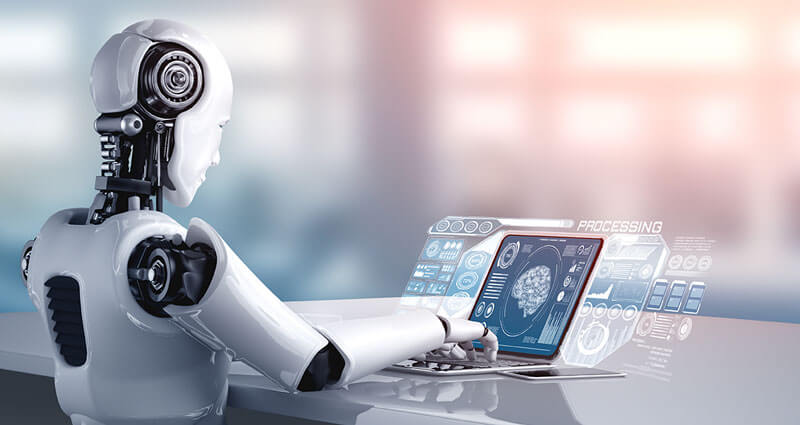
\includegraphics[width=\paperwidth,height=\paperheight]{supervised-vs-unsupervised-learning.jpg}}
	\begin{frame}[plain]
			% Contenu du frame
			\note{
			\textbf{Contexte actuel :}
			\begin{itemize}
				\item \textit{Forte demande en compétences en IA, ML et Deep Learning.}
				\item \textit{Jeunes diplômés cherchant à se préparer aux opportunités pro}
			\end{itemize}
			
			\textbf{Objectifs de la formation :}
			\begin{itemize}
				\item \textit{Fournir une introduction complète à l'IA, ML et Deep Learning.}
				\item \textit{Acquérir les compétences fondamentales en Python pour l'IA.}
				\item \textit{Comprendre les concepts et les algorithmes clés de l'IA et du ML.}
				\item \textit{Exploiter les bibliothèques populaires: Scikit Learn et TensorFlow}
				\item \textit{Appliquer les connaissances à des projets pratiques.}
			\end{itemize}
			
			\textbf{Résultats attendus :}
			\begin{itemize}
				\item \textit{Compétences solides en IA, ML et Deep Learning avec Python.}
				\item \textit{Capacité à résoudre des pbs réels en utilisant des techniques d'IA.}
				\item \textit{Préparation pour des opportunités professionnelles dans le domaine en pleine expansion de l'IA.}
			\end{itemize}
		}
	
		\titlepage
		
\includegraphics[scale=0.3]{BensearchLogo-removebg-preview.png}\hfill
		%	
\includegraphics[scale=0.7]{images}\hfill
			
\includegraphics[scale=0.1]{bensearch.png}	
	\end{frame}
}

\begin{frame}{Plan général de la présentation (AI and ML)}
	\begin{enumerate}
		\item Artifical Intelligence and Machine Learning 1
		\begin{itemize}
			\item Fondamentaux de l'IA et du Machine Learning
			\item Technical Approaches of AI in Machines Learning 
			\item Défis et évaluation des modèles 
		\end{itemize}
		\item Artifical Intelligence and Machine Learning 2
		\begin{itemize}
			\item Explicabilité de l'IA et IML
			\item Techniques d'explicabilité XAI et IML 
			\item Statistiques, causalité, et évaluation des modèles
		\end{itemize}
		\item Artifical Intelligence and Machine Learning 3
		\begin{itemize}
			\item Défis de l'IA et application étroite
			\item Apprentissage supervisé et non supervisé
			\item Explicabilité de l'IA (XAI) et traitement du langage naturel (NLP) 
		\end{itemize}
		\item Artifical Intelligence and Machine Learning 4 : Cas Pratiques
		\begin{itemize}
			\item Analyse de données avec Power BI 
			\item Chatbots avec Azure et Google Dialogflow
			\item Apprentissage automatique avec Scikit-Learn 
		\end{itemize}
	\end{enumerate}	
\end{frame}

\begin{frame}{Plan général de la présentation (Python)}
\begin{enumerate}
	\item Python for Machine Learning 1 : Initialization
	\item Python for Machine Learning 2 : Advanced
	\item Deep Learning and Neural Network
\end{enumerate}
\end{frame}


\section{Introduction à l'IA et au Machine Learning}
\subsection{Qu'est ce que l'IA?}
\subsection{Qu'est ce que le Machine Learning?}
\subsection{Difference entre le Machine Learning et l'IA}
\subsection{Histoire de l'IA}
\subsection{Approches techniques de l'IA}
\subsection{L'IA en robotique}
\subsection{Introduction au Big Data et son intégration avec l'IA}
\subsection{Concepts de base de l'apprentissage automatique}
\subsection{Types de Machine Learning}
\subsection{Travailler avec les données}
\subsection{Préparation des données pour l'apprentissage automatique}

{
	\setbeamertemplate{background}{
\includegraphics[width=\paperwidth,height=\paperheight]{ia_ml.jpg}}
\begin{frame}[plain]{Artificial Intelligence and Machine Learning 1}
%	\centering
%
\includegraphics[width=\linewidth]{ia_ml.jpg}
\end{frame}
}	% Page de titre
	%\begin{frame}
	%		\titlepage
	%\end{frame}

	%	\frametitle{Questions clés pour comprendre l'impact quotidien de l'IA}
	%\section{Artificial Intelligence and Machine Learning 1}
	\section{Introduction à l'IA et au Machine Learning}
\begin{frame}
	\frametitle{Introduction à l'IA et au Machine Learning}
	\begin{itemize}
		\item Qu'est ce que l'Intélligence Artificielle?
		\item Histoire de l'Intélligence Artificielle
		\item Machine Learning
		\item L'Intélligence Artificielle en robotique
		\item Introduction au Big Data et son intégration avec l'IA
		%\item Concepts de base de l'apprentissage automatique
		%\item Types d'apprentissage automatique
		\item Éviter les pièges et travailler avec les données
		\item Principes du Machine Learning
		\item Avantages et inconvénients de l'IA et du ML
		\item Conclusion 
	\end{itemize}
\end{frame}

\subsection{Qu'est ce que l'IA?}
\begin{frame}{Questions clés pour comprendre l'impact quotidien de l'IA}
 
   \note{
 	\begin{itemize}
 		\item \textit{\textbf{La reconnaissance faciale} utilise des algorithmes d'apprentissage automatique (ML) que nous explorerons dans cette formation pour extraire des caractéristiques faciales uniques, telles que la distance entre les yeux, la forme du nez, etc. Ces caractéristiques sont ensuite comparées à une base de données pour trouver une correspondance.}
 		
 		\item 
 		\textit{\textbf{Les chatbots} utilisent des techniques d'IA telles que le traitement du langage naturel (NLP) et l'apprentissage automatique pour comprendre les messages des utilisateurs, générer des réponses appropriées et améliorer leur performance au fil du temps.}
 	\end{itemize}
 }	
	\begin{figure}[h]
		\centering
		\begin{minipage}{0.48\textwidth}
			\centering
			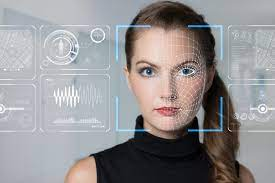
\includegraphics[width=\linewidth]{rf.jpeg}
			\caption{Reconnaissance faciale}
		\end{minipage}\hfill
		\begin{minipage}{0.48\textwidth}
			\centering
			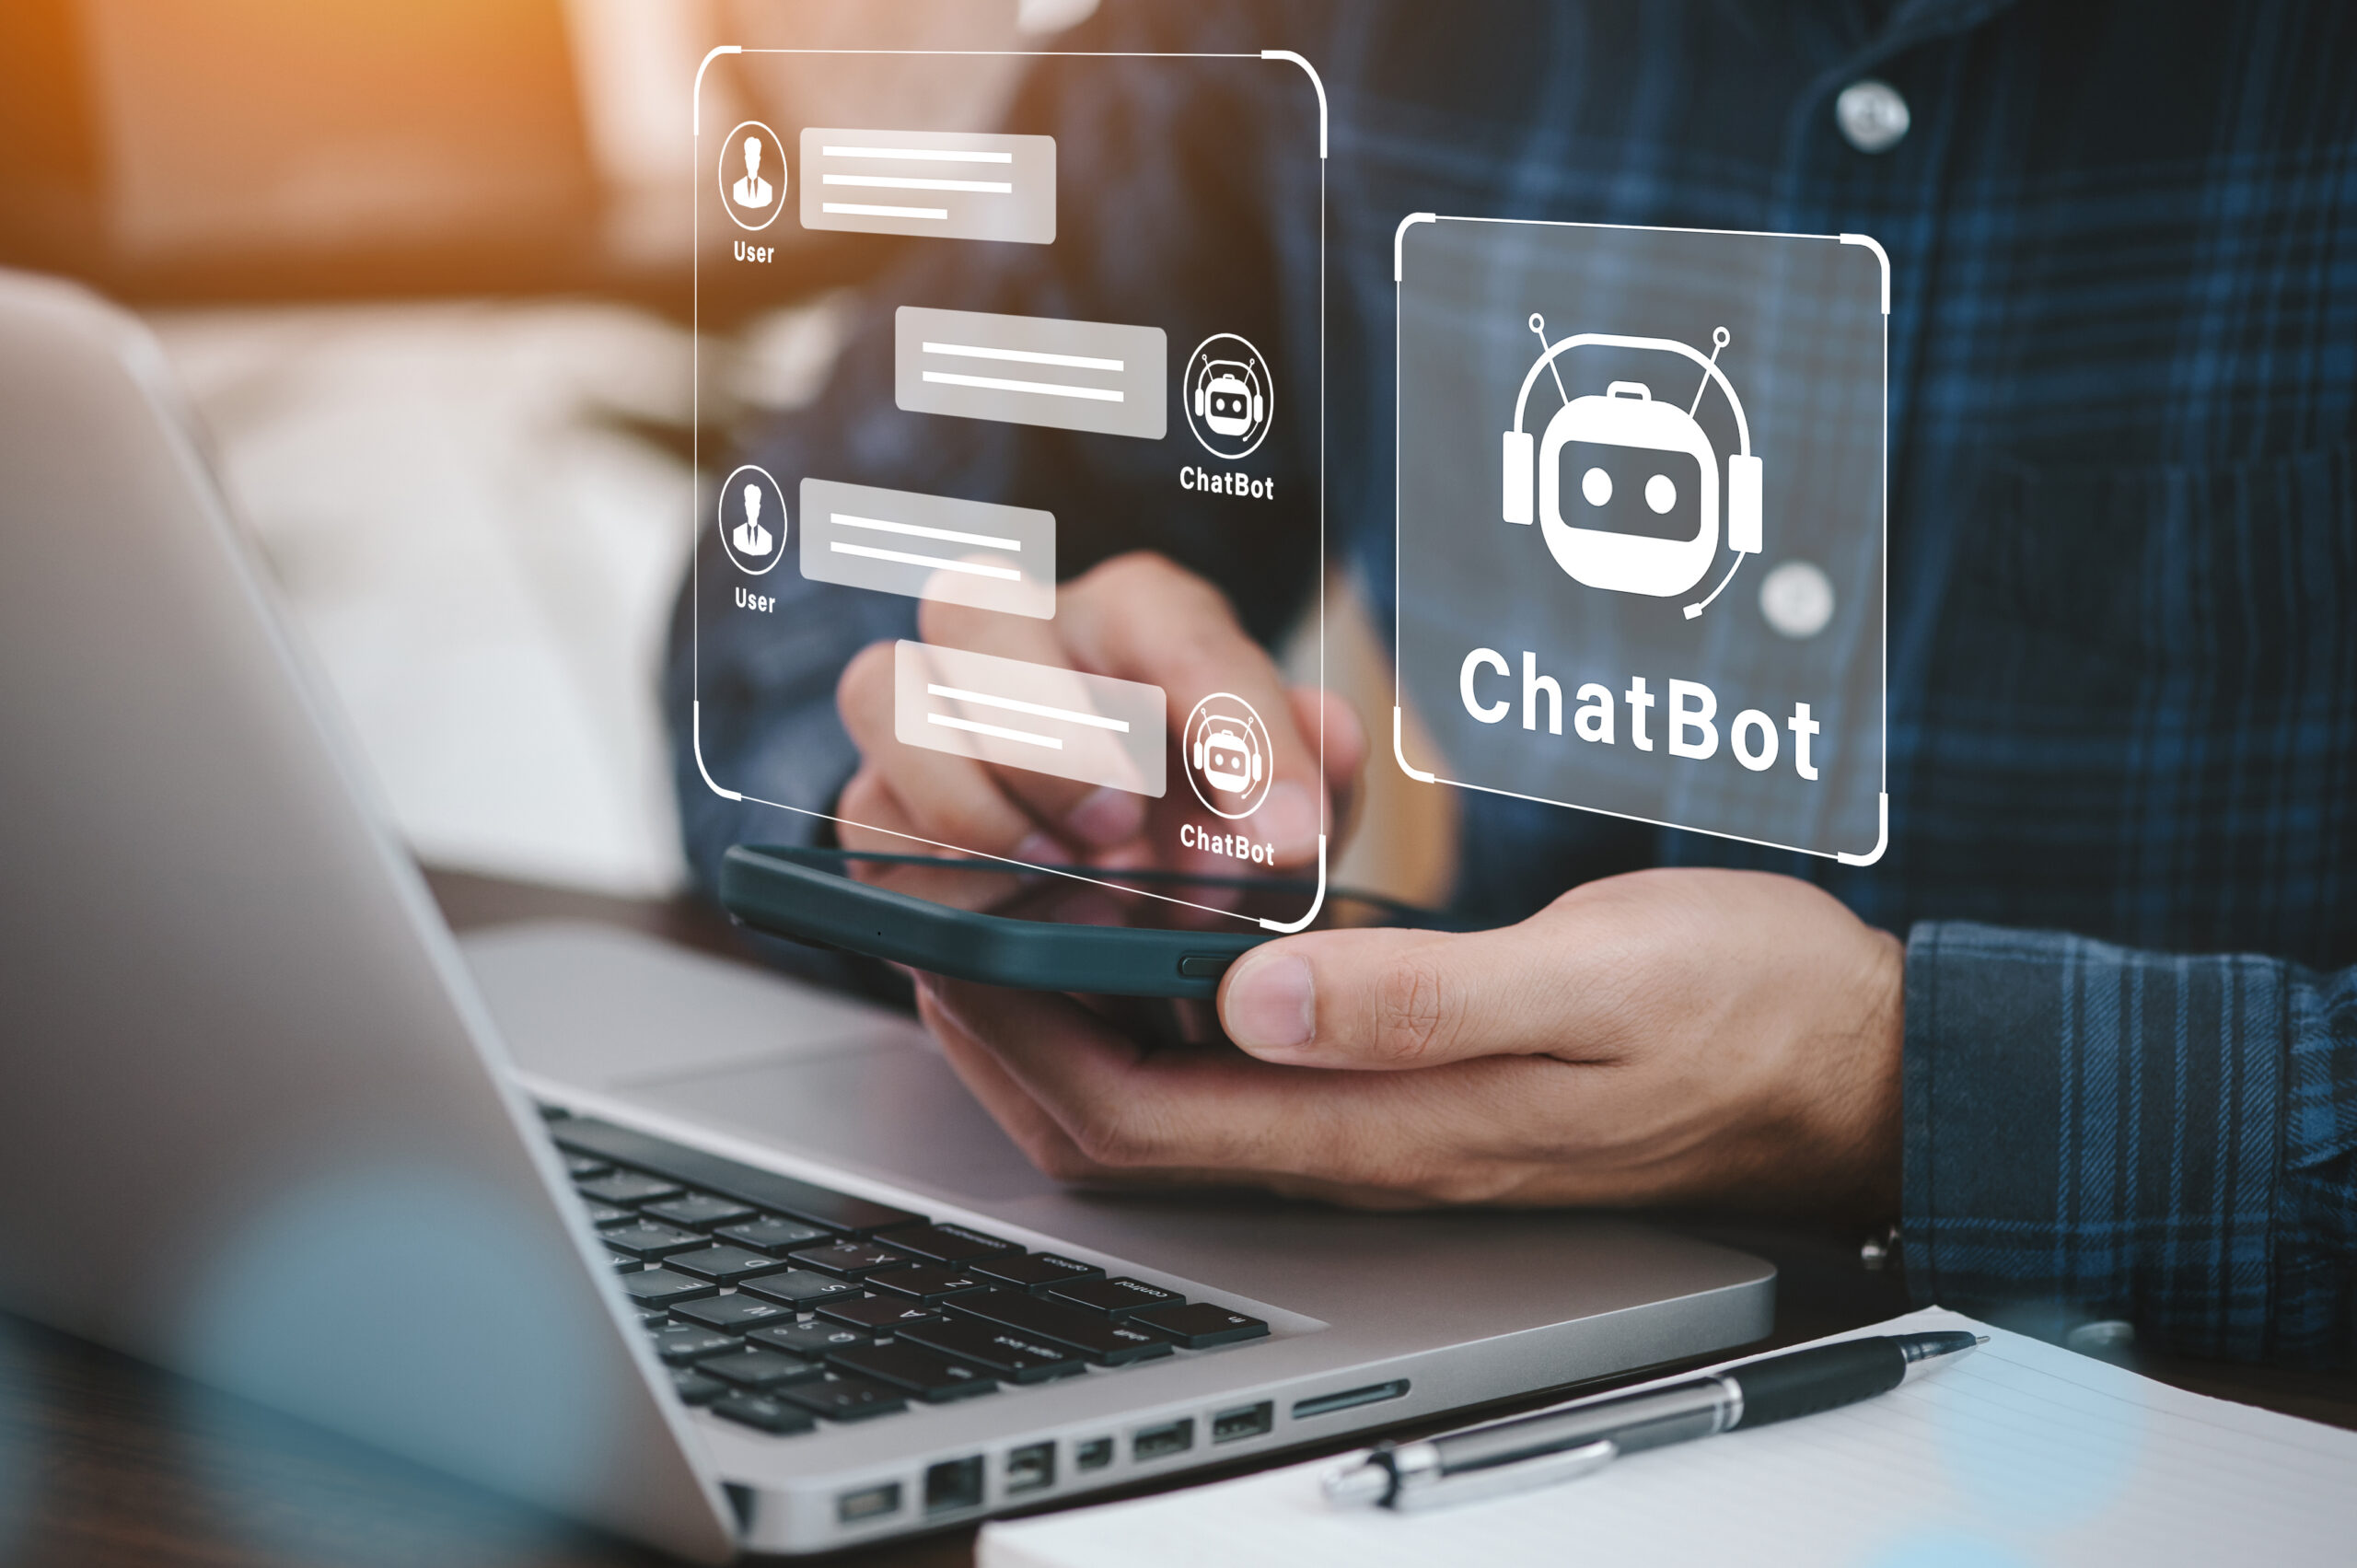
\includegraphics[width=\linewidth]{ChatBot.jpg}
			\caption{Application de chatbot}
		\end{minipage}

	\end{figure}

\end{frame}



\begin{frame}{Questions clés pour comprendre l'impact quotidien de l'IA}
	  \note{
		\begin{itemize}
			\item \textit{\textbf{La classification d'emails} utilise des techniques d'IA, comme l'apprentissage supervisé, pour prédire les catégories des nouveaux messages en se basant sur des ensembles de données étiquetés (Grand ensemble d'emails classifiés comme \textbf{INBOX} ou \textbf{SPAM})}.
			
			\item \textit{\textbf{La suggestion d'amis Facebook} utilise des algorithmes d'apprentissage automatique  pour analyser les profils d'utilisateurs, leurs interactions et leurs intérêts communs afin de proposer des suggestions pertinentes de connexions amicales sur la plateforme.}
		\end{itemize}
	}
\begin{figure}
	\begin{minipage}{0.48\textwidth}
	\centering
	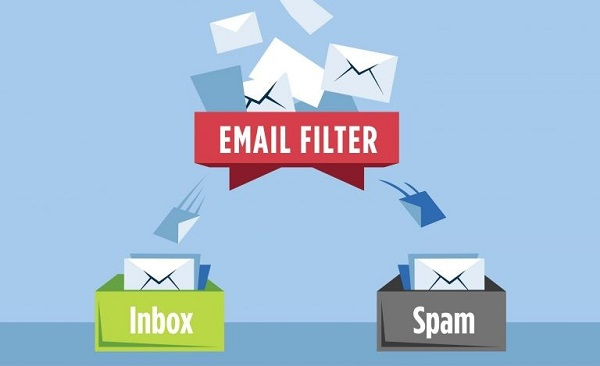
\includegraphics[width=\linewidth]{spam-1.jpg}
	\caption{Classification d'emails}
\end{minipage}\hfill
\begin{minipage}{0.44\textwidth}
	\centering
	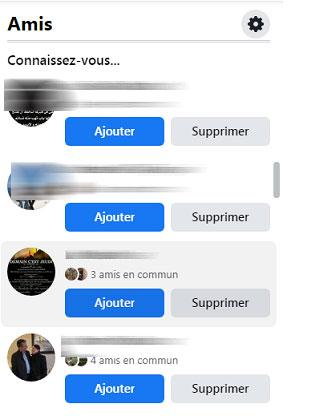
\includegraphics[width=\linewidth]{connaissez-vous-facebook.jpg}
	\caption{Suggestion d'amis facebook}
\end{minipage}
\end{figure}
\end{frame}
	%	\begin{itemize}
		%	\item Comment les systèmes de recommandation personnalisée fonctionnent-ils pour suggérer des produits, des films ou de la musique adaptés à nos préférences ?
	%		\item Comment les voitures autonomes sont-elles capables de détecter et de réagir aux obstacles sur la route de manière autonome ?
	%		\item Comment les applications de traduction instantanée parviennent-elles à convertir automatiquement un texte d'une langue à une autre ?
	%		\item Comment les assistants virtuels, tels que Siri ou Google Assistant, comprennent-ils nos commandes vocales et fournissent-ils des réponses pertinentes ?
	%		\item Comment les moteurs de recherche sont-ils en mesure de fournir des résultats personnalisés et pertinents en fonction de notre historique de recherche ?
	%		\item Comment les systèmes de reconnaissance faciale sont-ils capables d'identifier et de reconnaître les visages dans les photos ou les vidéos ?
	%		\item Comment les applications de chatbot utilisent-elles l'apprentissage automatique pour comprendre et répondre aux questions des utilisateurs de manière conversationnelle ?
		%	\item Comment les systèmes de détection de fraude analysent-ils les modèles d'activité pour identifier les transactions suspectes ?
		%	\item Comment les filtres anti-spam des boîtes e-mail sont-ils capables de trier les messages indésirables des messages légitimes ?
	%		\item Comment les applications de reconnaissance vocale transforment-elles nos paroles en texte de manière précise et rapide ?
	%	\end{itemize}

		
	\begin{frame}
		\frametitle{Questions clés pour comprendre l'impact quotidien de l'IA}
	\note{
	\textit{	\textbf{Les voitures autonomes} utilisent des capteurs tels que des caméras, des lidars et des radars pour détecter les obstacles sur la route.\\ Les données fournis par ces capteurs sont traitées par des algorithmes de ML qui reconnaissent les objets et prennent des décisions en temps réel, comme le freinage ou l'évitement d'obstacles. L'IA permet aux voitures autonomes d'apprendre et de s'améliorer avec l'expérience pour une conduite plus sûre et efficace.}
	}	
		\begin{figure}[h]
			\centering
			\begin{minipage}{0.5\textwidth}
				\centering
				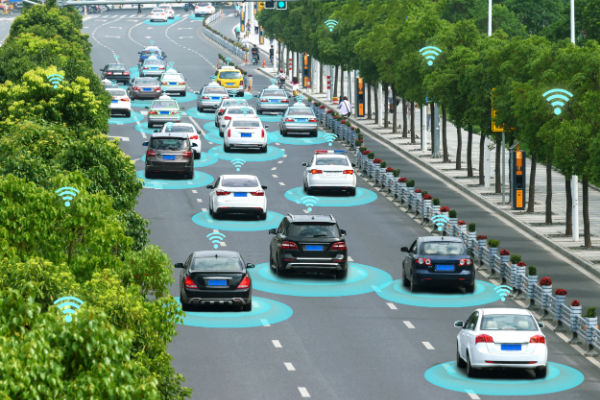
\includegraphics[width=\linewidth]{voiture-autonome.jpg}
				\caption{Voiture autonome}
			\end{minipage}\hfill
			\begin{minipage}{0.5\textwidth}
				\centering
				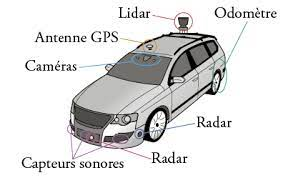
\includegraphics[width=\linewidth]{voitureauto.jpeg}
				\caption{Composantes }
			\end{minipage}
		\end{figure}
	Comment les voitures autonomes sont-elles capables de détecter et de réagir aux obstacles sur la route de manière autonome?
		
	\end{frame}	
		
		
	\begin{frame}{Questions clés pour comprendre l'impact quotidien de l'IA}
		
		  \note{
			\begin{itemize}
				\item \textit{\textbf{L'assistant personnel de Microsoft} utilise le NLP et le ML, pour comprendre les requêtes des utilisateurs et fournir des réponses et des actions pertinentes. Il s'améliore également en apprenant des interactions passées.}
				
				\item \textit{\textbf{Les applications de reconnaissance vocale} utilisent le ML pour convertir la parole en texte, utilisés dans des applications, comme les assistants vocaux.}
				
				\item \textit{\textbf{Les applications de traduction instantanée} utilisent des techniques d'IA, telles que les réseaux de neurones, pour traduire automatiquement du texte ou de la parole d'une langue à une autre en temps réel.}
				
				\item \textit{\textbf{Les résultats de recherche personnalisés} utilisent le ML pour analyser les préférences et le comportement de l'utilisateur, afin de fournir des résultats de recherche plus pertinents et personnalisés en fonction de ses intérêts et de son historique.}
			\end{itemize}
		}
		
		\begin{figure}[h]
			\centering
			\begin{minipage}{0.4\textwidth}
				\centering
				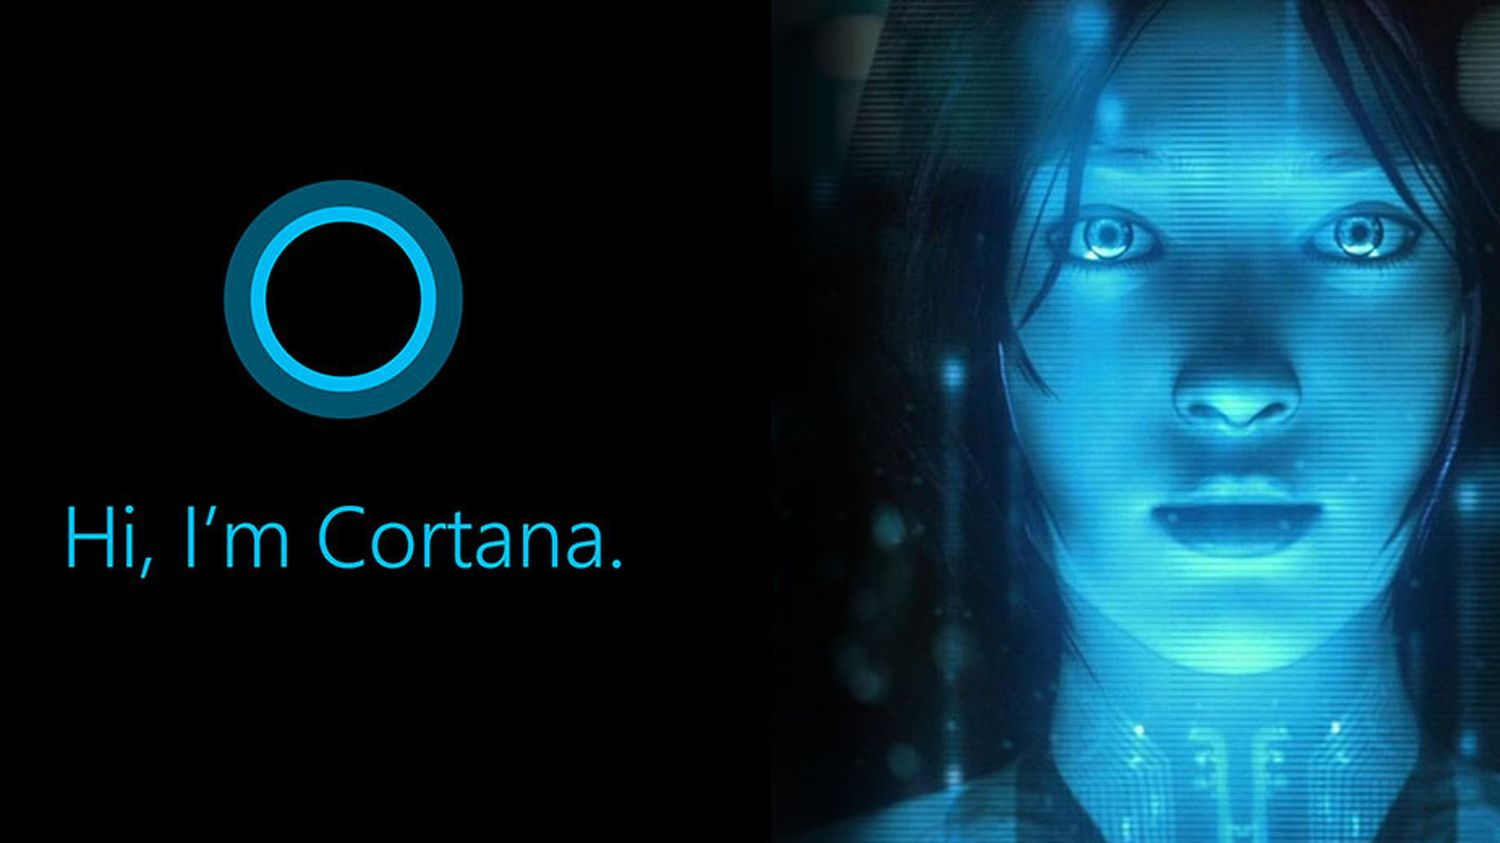
\includegraphics[width=\linewidth]{cortana_.jpg}
				\caption{Assistant personnel intelligent de MS}
			\end{minipage}\hfill
			\begin{minipage}{0.34\textwidth}
				\centering
				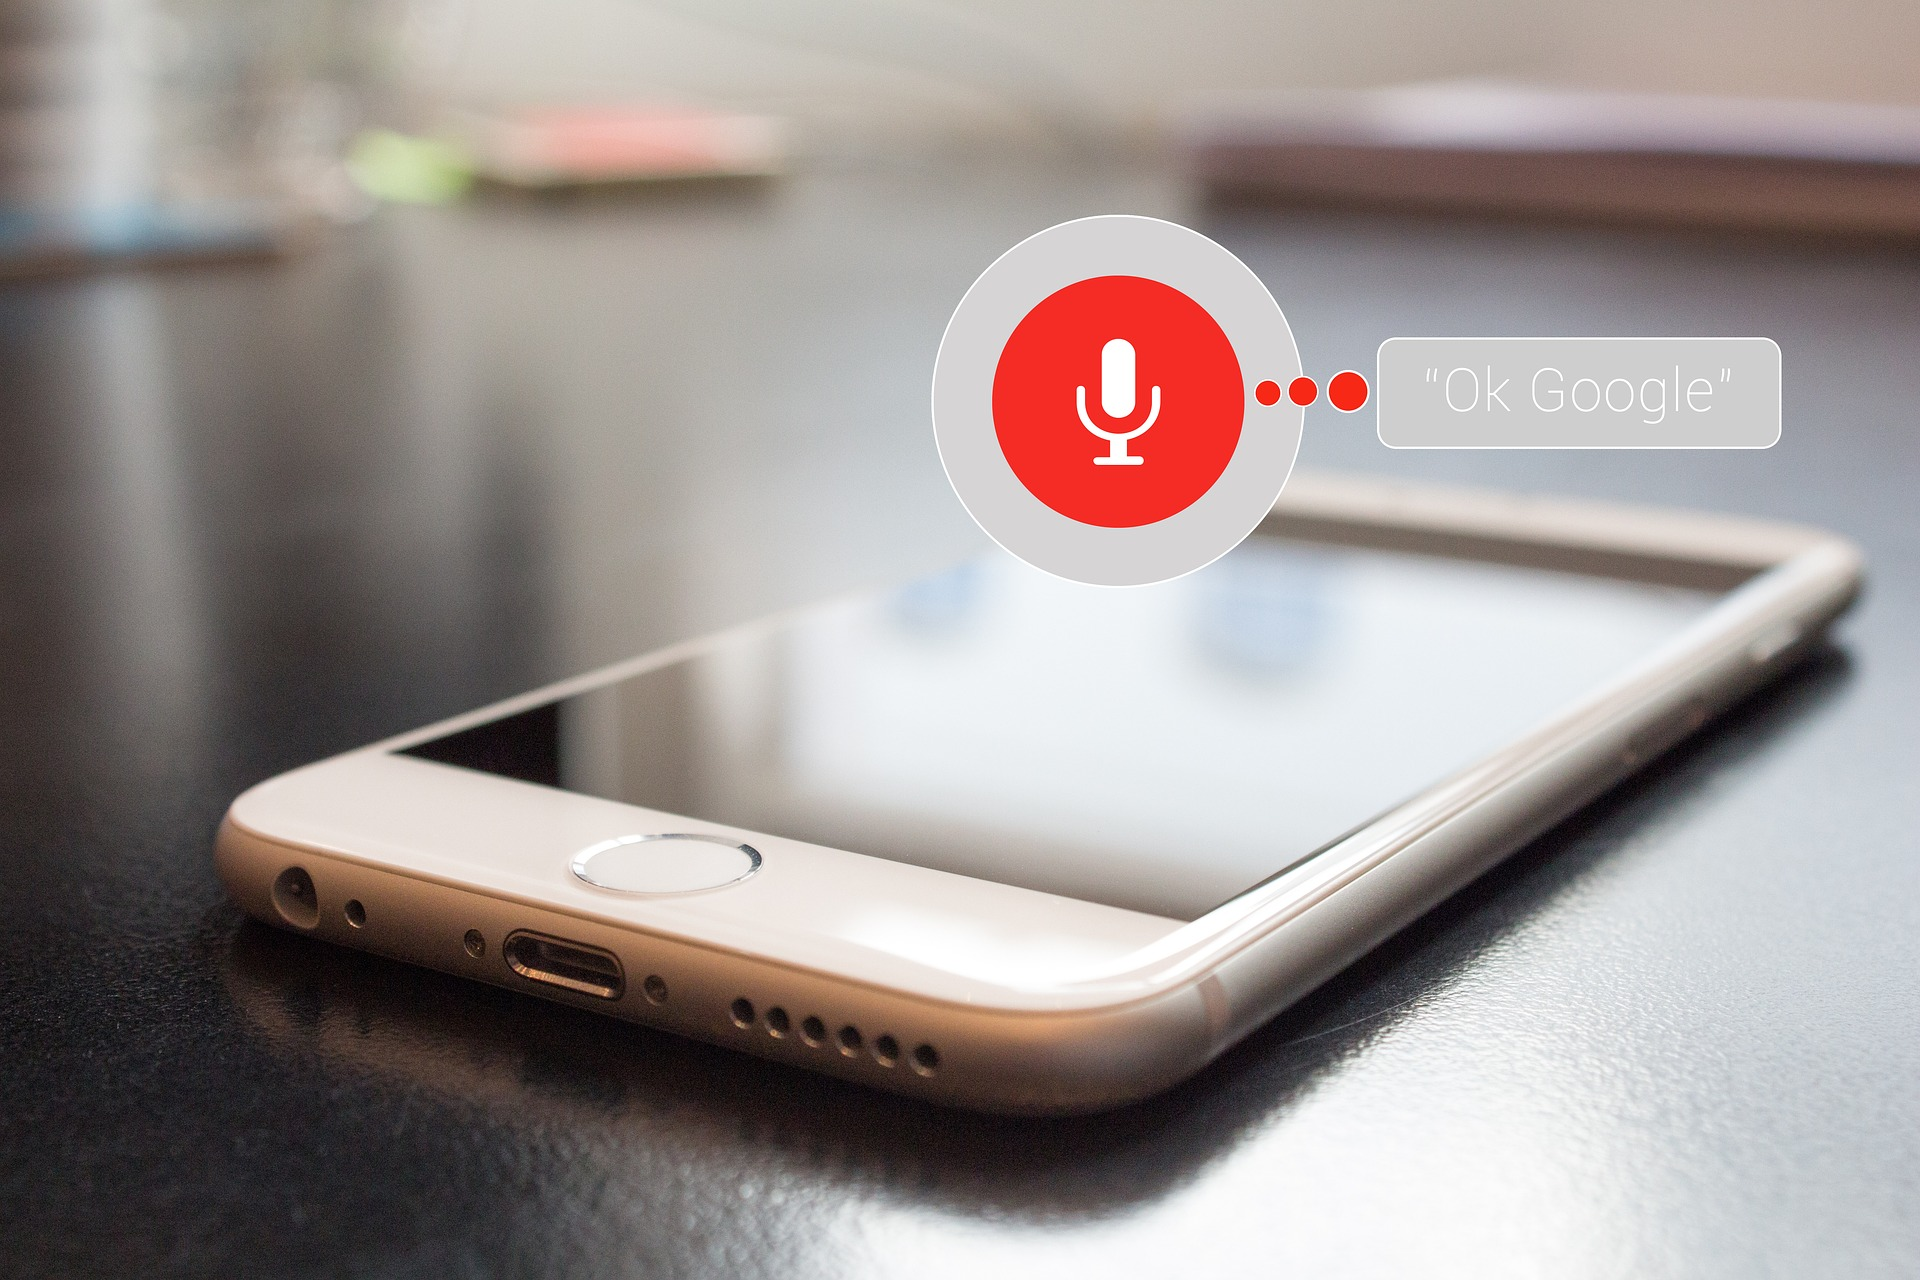
\includegraphics[width=\linewidth]{voice-control.jpg}
				\caption{Applications de reconnaissance vocale}
			\end{minipage}
			\vspace{0.5cm}
			\begin{minipage}{0.4\textwidth}
				\centering
				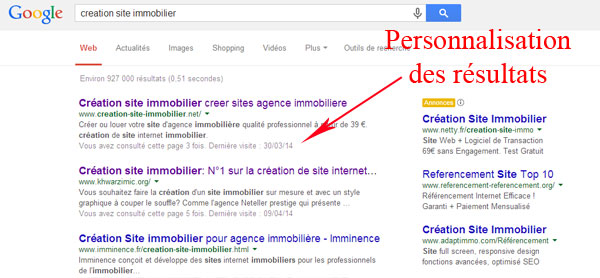
\includegraphics[width=\linewidth]{personnalisation.jpg}
				\caption{Resultat de recherche personalisée}
			\end{minipage}\hfill
			\begin{minipage}{0.32\textwidth}
				\centering
				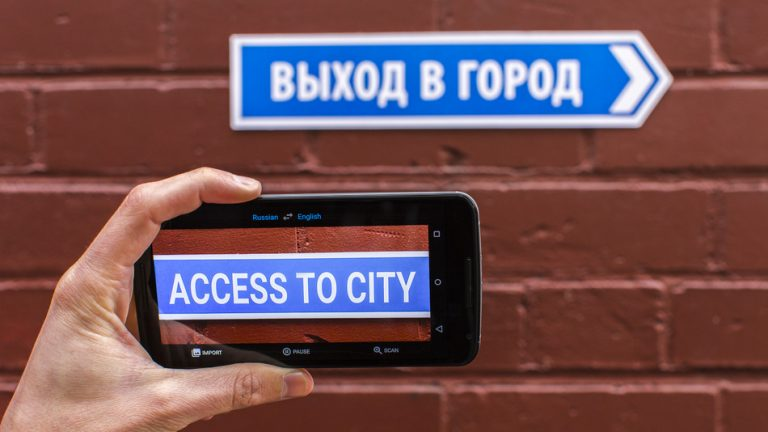
\includegraphics[width=\linewidth]{googlet.jpg}
				\caption{Application de traduction instantanée}
			\end{minipage}
		\end{figure}
		
	\end{frame}	
		
{
	\setbeamertemplate{background}{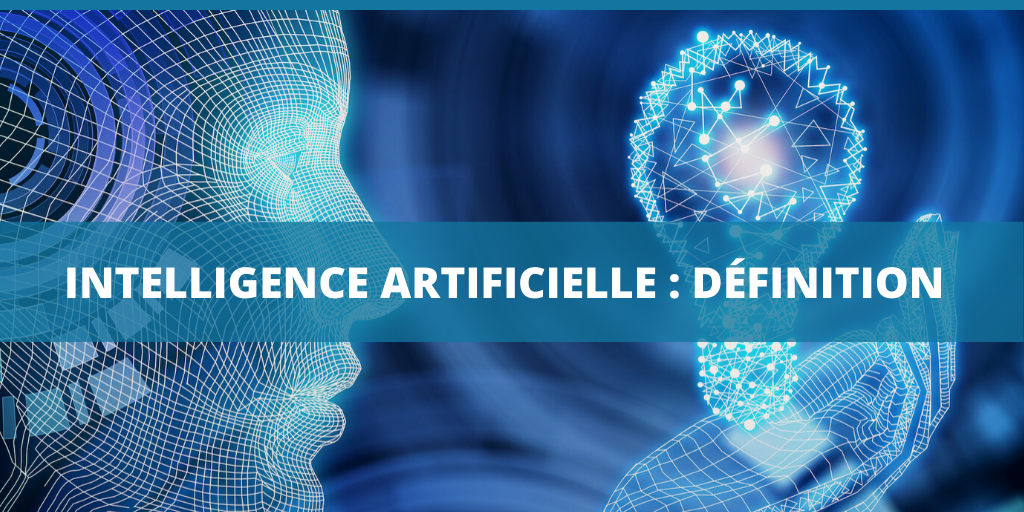
\includegraphics[width=\paperwidth,height=\paperheight]{defia.png}}
	\begin{frame}[plain]{Comment définiriez-vous l'IA en vos propres termes ?}
		%	\centering
		%
\includegraphics[width=\linewidth]{ia_ml.jpg}
	\end{frame}
}

{
	\setbeamertemplate{background}{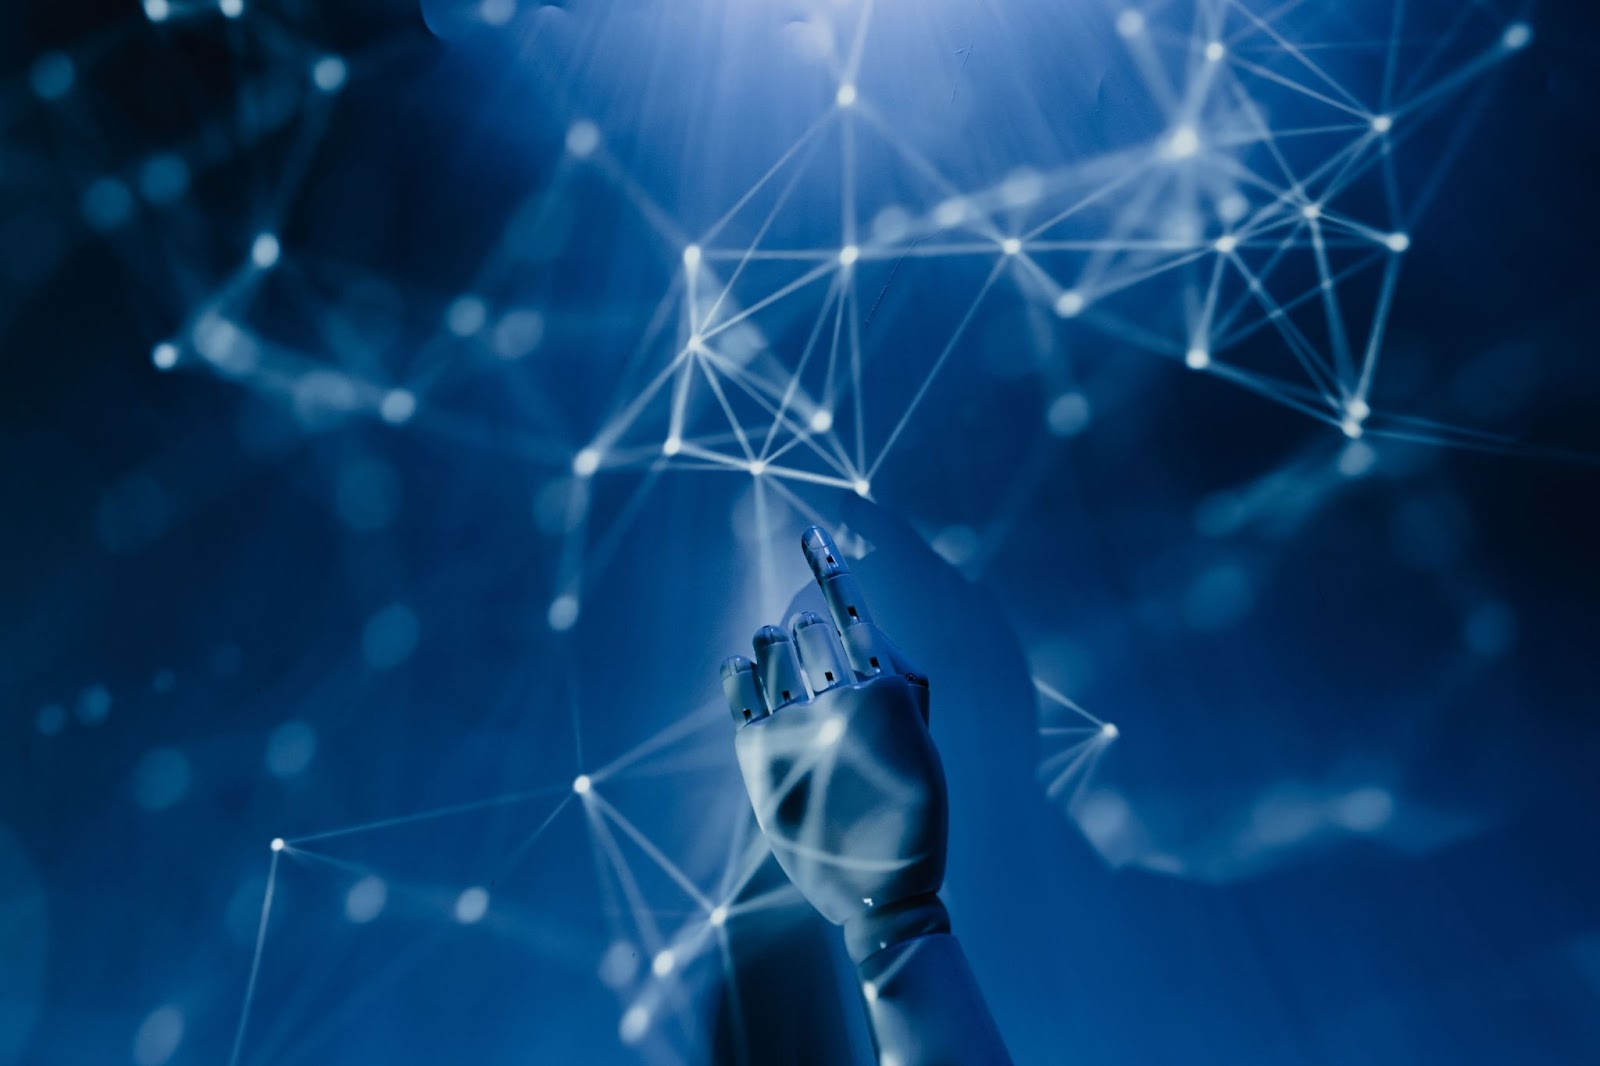
\includegraphics[width=\paperwidth,height=\paperheight]{bakiadef.jpeg}}
\begin{frame}
	\frametitle{Définition de l'IA selon quelques auteurs}
	\begin{itemize}
\color{white}		\item \textbf{John McCarthy (1956)} : "L'IA est la science et l'ingénierie de la création de machines intelligentes, qui ont la capacité de réaliser des tâches qui nécessitent normalement l'intelligence humaine."
\vspace{0.3cm}
		\item \textbf{Stuart Russell et Peter Norvig (2009)} : "L'IA est le domaine de l'informatique qui traite de la création et de l'étude de machines qui peuvent effectuer des tâches qui, si elles étaient accomplies par des êtres humains, nécessiteraient de l'intelligence."
		\vspace{0.3cm}
		\item \textbf{Marvin Minsky (1968)} : "L'IA est la construction de programmes informatiques qui peuvent accomplir des tâches qui, lorsqu'elles sont accomplies par des personnes, demandent de l'intelligence."
	\end{itemize}
	
\end{frame}
}	% Slide 2: Introduction



	% Slide 3: Objectifs du projet
	\subsection{Histoire de l'IA}
	\begin{frame}{Les dates clés de l'Intelligence Artificielle}
		\note{
			\begin{itemize}
			
				\item \textbf{1965 :} Joseph Weizenbaum crée ELIZA, un programme de traitement du langage naturel qui simule une conversation psychothérapeutique.
				\item \textbf{1969 :} Marvin Minsky et Seymour Papert publient le livre "Perceptrons", qui met en évidence les limites du perceptron et freine temporairement le développement des réseaux de neurones.
				\item \textbf{1973 :} James Lighthill publie le rapport Lighthill, critiquant les progrès insuffisants de l'IA et entraînant une période de désintérêt et de financement réduit pour le domaine.
				\item \textbf{1974 :} Ted Shortliffe développe MYCIN, un système expert utilisé pour le diagnostic et le traitement des infections bactériennes.
			\end{itemize}
		}
		\centering
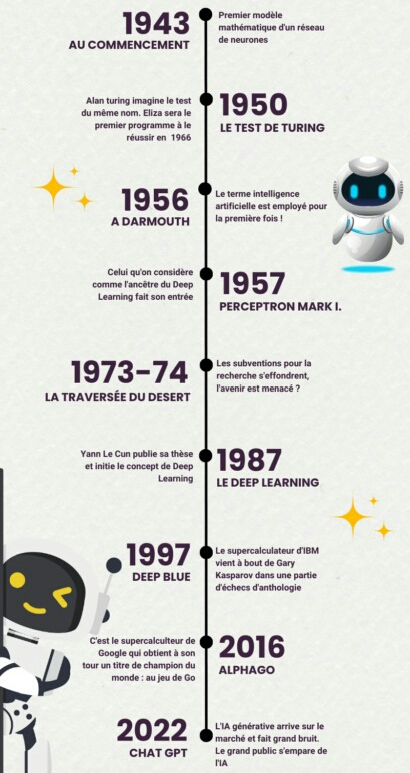
\includegraphics[width=0.6\linewidth]{AIhistory.jpeg}
%\caption{Les dates clés de l'Intelligence Artificielle}
	\end{frame}

%	\subsection{Histoire de l'IA}
\begin{frame}{Les dates clés de l'Intelligence Artificielle}
	\note{
		\begin{itemize}


			\item \textbf{2014 :} Les réseaux de neurones récurrents (RNN) deviennent populaires pour le traitement des séquences, ouvrant la voie à des applications telles que la traduction automatique et la génération de texte.
			\item \textbf{2018 :} GPT-2 (Generative Pre-trained Transformer 2), un modèle basé sur l'apprentissage non supervisé, fait sensation en générant du texte de manière presque indiscernable de l'écriture humaine.
			\item \textbf{2020 :} L'IA de génération de texte, GPT-3, développée par OpenAI, impressionne par sa capacité à produire du texte créatif et convaincant dans une variété de domaines.
			\item \textbf{2022 :} OpenAI lance DALL·E, un modèle de génération d'images capable de créer des illustrations à partir de descriptions textuelles, repoussant les limites de la créativité des machines.
		\end{itemize}

	}
	\centering
	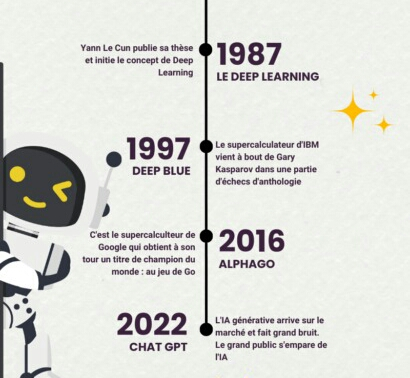
\includegraphics[width=0.6\linewidth]{hia.jpeg}
	%\caption{Les dates clés de l'Intelligence Artificielle}
\end{frame}


{
	\setbeamertemplate{background}{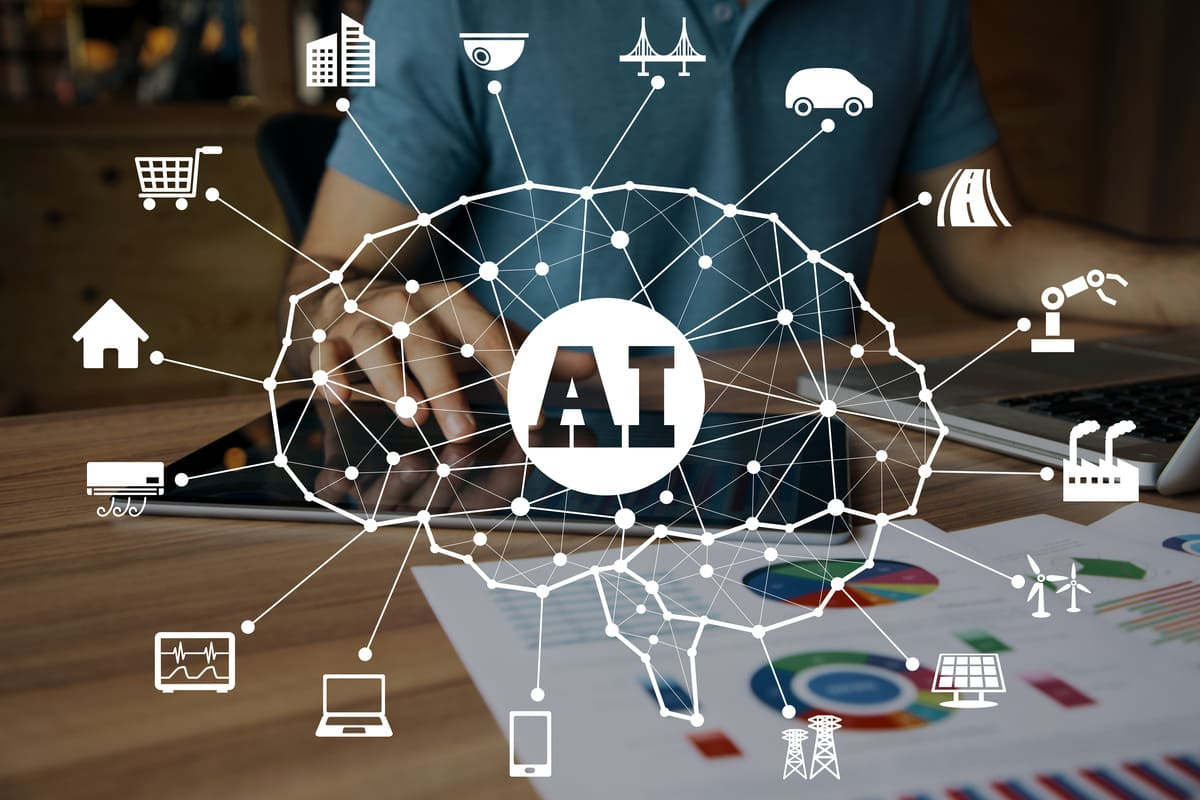
\includegraphics[width=\paperwidth,height=\paperheight]{AI actu.jpeg}}
\begin{frame}{Exercice sur l'histoire de l'IA}
	Pourquoi c'est à nos jours que l'IA fait la une de l'actualité, alors que les fondements mathématiques des réseaux de neurones remontent à 1943 ?
	\note{L'IA fait aujourd'hui la une de l'actualité pour plusieurs raisons clés:
		\begin{itemize}
	
			\item \textit{\textbf{Progrès techniques :} Les récentes avancées en matière de puissance de calcul, de stockage de données et d'algorithmes ont permis de développer des systèmes d'IA beaucoup plus performants.}
			\item \textit{\textbf{Données massives :} L'explosion du volume de données disponibles, grâce à l'Internet et aux appareils connectés, alimente l'entraînement des modèles d'IA.}
			\item \textit{\textbf{Applications concrètes :} L'IA peut maintenant être déployée dans de nombreux domaines (santé, transport, finance, etc.), démontrant son utilité pratique.}
			\item \textit{\textbf{Prise de conscience publique :} Les médias et le grand public s'intéressent davantage à l'IA et à son impact potentiel, alimentant le débat.}
	\end{itemize}}
\end{frame}
}

\begin{frame}{Les Intelligences Artificielles populaires }
	\note{
		\begin{itemize}
	\item \textbf{TCHATGPT} : \textit{TCHATGPT est un modèle de langage développé par OpenAI. Il est conçu pour répondre de manière interactive aux questions et aux conversations.}
			
			
		\item \textbf{Jasper Chat} : \textit{Jasper Chat est un assistant vocal développé par Jasper Technologies. Il est utilisé pour la réservation de rendez-vous, la gestion des tâches,...
		}
		\item \textbf{Getgenie} : \textit{Getgenie est un assistant vocal développé par Genie AI. Il est conçu pour aider les utilisateurs à gérer leurs e-mails en utilisant des commandes vocales, notamment la recherche, le tri et la réponse aux messages.}
		
		\item \textbf{Simplified} : \textit{Simplified est une IA développée par Simplified AI. Elle est utilisée pour automatiser les tâches de service client, en fournissant des réponses automatisées aux requêtes des clients et en les redirigeant vers les ressources appropriées.}	
		\end{itemize}
			
		}
	\centering
	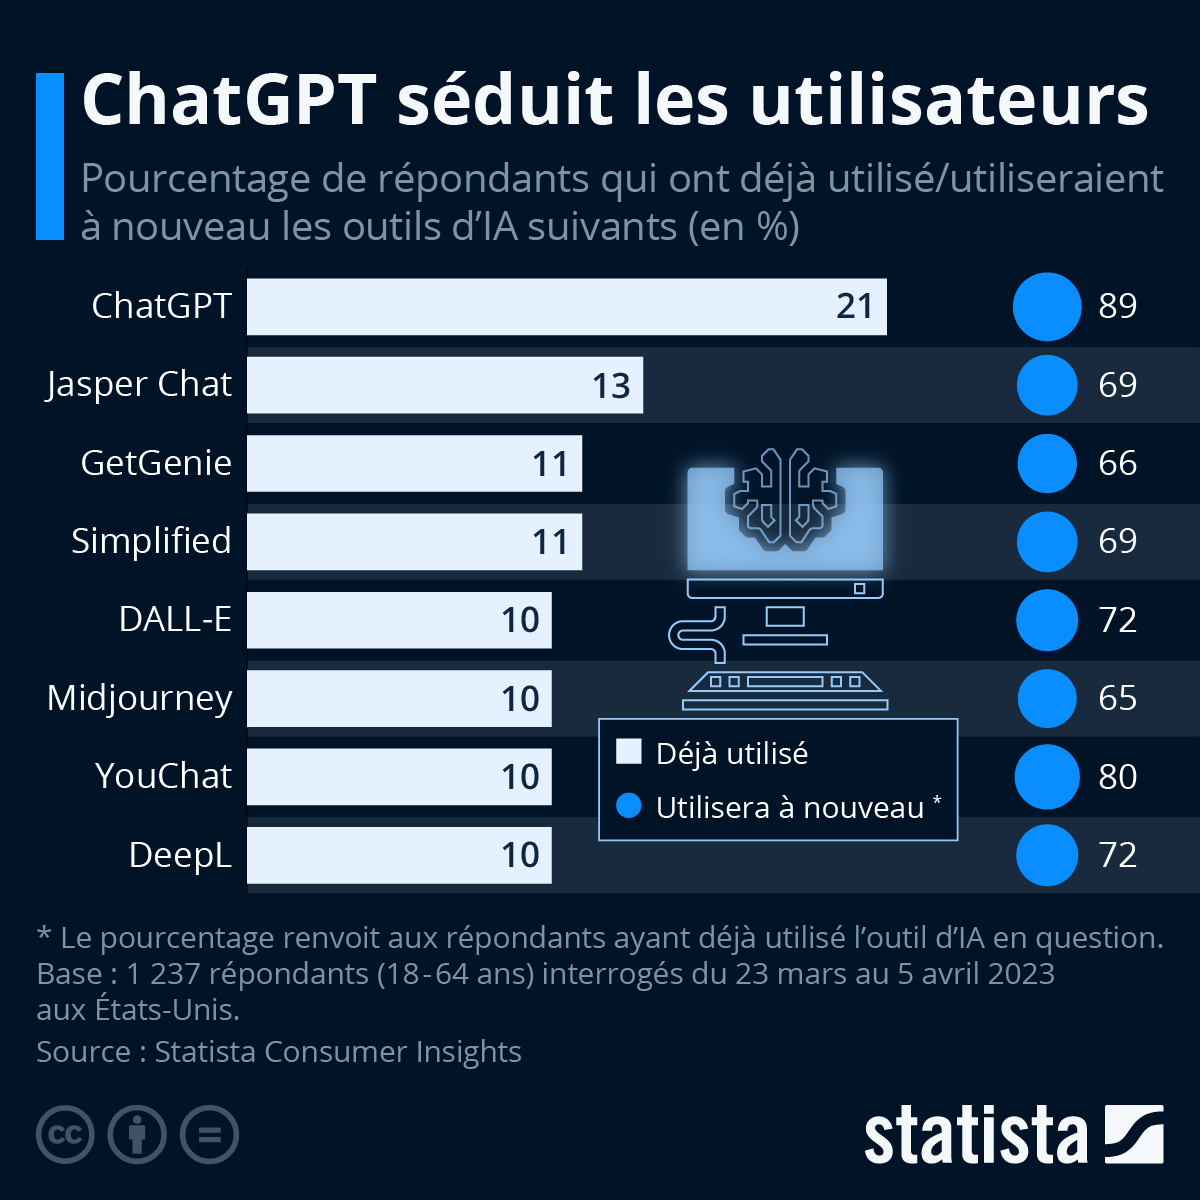
\includegraphics[width=0.6\linewidth]{PopularAI.jpeg}
	%\caption{Les dates clés de l'Intelligence Artificielle}
\end{frame}


\begin{frame}{La course vers les brevets}
	\note{\begin{itemize}
					\item \textbf{DALL-E} : \textit{DALL-E est un modèle d'IA développé par OpenAI. Il est spécialisé dans la génération d'images à partir de descriptions textuelles, permettant de créer des images réalistes et créatives basées sur des concepts abstraits.}
			
			\item \textbf{Midjourney} : \textit{Midjourney est une plateforme d'IA utilisée dans le domaine du commerce électronique. Elle utilise l'apprentissage automatique pour analyser les données des clients, recommander des produits et optimiser les stratégies de vente.}
			
			\item \textbf{Youchat} : \textit{Youchat est une IA développée par YouAI. Elle est utilisée pour créer des chatbots conversationnels personnalisés qui peuvent interagir avec les utilisateurs, répondre aux questions et fournir des informations en temps réel.}
			
			\item \textbf{DeepL} : \textit{DeepL est un service de traduction en ligne basé sur l'IA. Il offre des traductions précises et naturelles dans plusieurs langues, grâce à des modèles de traduction neuronaux avancés.}
	\end{itemize}}
	\centering
	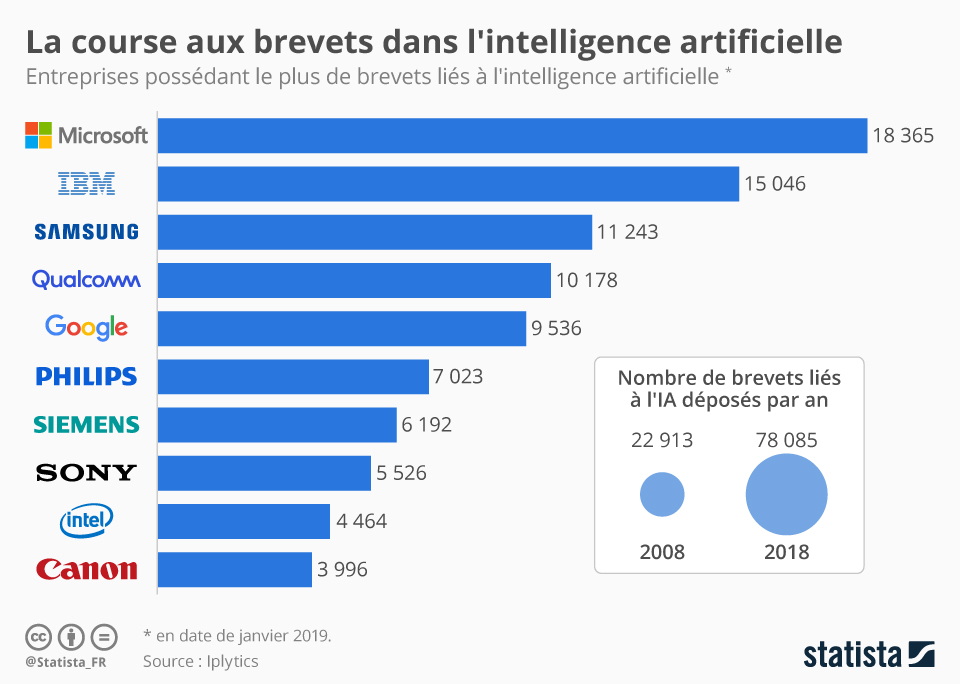
\includegraphics[width=\linewidth]{BrevetIA.jpeg}
	%\caption{Les dates clés de l'Intelligence Artificielle}
\end{frame}


\begin{frame}{Future de l'IA}
	\framesubtitle{Que penser de son impact future dans notre socièté?}
	\note{
		\begin{itemize}
			\item \textit{Amélioration des capacités de traitement du langage naturel, ce qui permettra une communication plus fluide entre les humains et les machines, facilitant ainsi l'interaction avec les systèmes d'IA dans divers domaines tels que les assistants virtuels et les traducteurs automatiques.}
			\item \textit{Avancées dans la compréhension et la génération de contenu multimédia: création artistique, divertissement, réalité virtuelle.}
			\item \textit{Améliorations significatives d'efficacité, de précision et de prise de décision.
			\item Systèmes plus autonomes et capables de s'adapter à des situations changeantes.}
			\item \textit{Systèmes d'IA respectant les normes éthiques et les valeurs humaines, confiance et acceptation sociale de ces technologies.}
	\end{itemize}
}
	\centering
	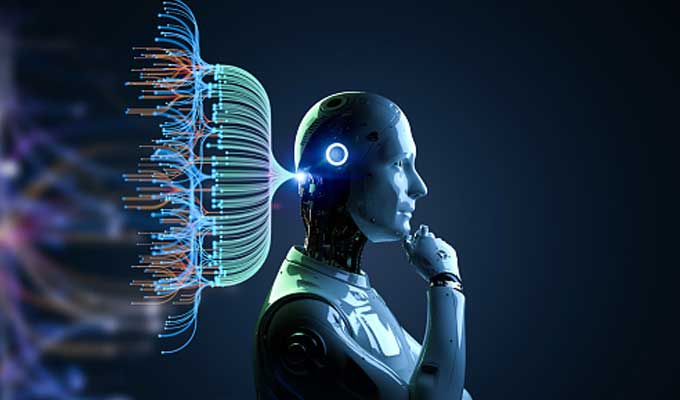
\includegraphics[width=\linewidth]{Fut.jpg}
	%\caption{Les dates clés de l'Intelligence Artificielle}
\end{frame}

\subsection{Qu'est ce que le Machine Learning?}
		\begin{frame}{Qu'est ce que le Machine Learning}
	
	\note{
		\begin{itemize}
		
		\item \textit{Le Machine Learning peut être défini comme étant une technologie d’IA permettant aux machines d’apprendre sans avoir été préalablement programmées spécifiquement à cet effet.}
		
		\item  \textit{Ledit apprentissage est fait sur les données, à titre d'illustration une banque disposant d'informations pertinantes sur des personnes ayant empreinté de l'argent autrefois est en mesure d'entrainer une machine à detecter à priori si quelqu'un est un "\textbf{GOOD or BAD credit risk}"}
		
		
		\item \textit{C'est donc tout processus par lequel un système améliore ses performances à partir de l'expérience issue des données.}
			
	\end{itemize}
	
}
	\centering
	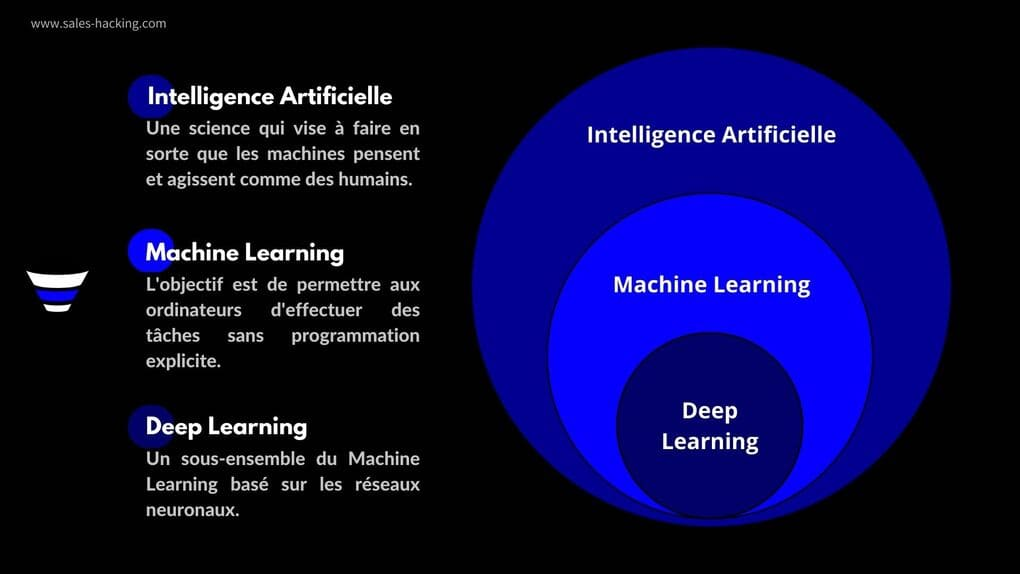
\includegraphics[width=\linewidth]{compar.png}
	%	\begin{block}{Différence entre l'IA et le Machine Learning}		
	\end{frame}

\subsection{Approches techniques de l'IA utilisées dans le ML}
\begin{frame}{Approches techniques de l'IA utilisées dans le ML}
	
	\note{On distingue trois grandes catégories de ML
		
		\begin{itemize}
			\item \textbf{Supervised Learning (Apprentissage supervisé)}
			\begin{itemize}
				\item \textit{Entraînement à partir de données étiquetées}
				\item \textit{La \textbf{régression} pour prédiction de valeurs continues et la \textbf{classification} de catégories }
				\item \textit{Généralisation des schémas pour prédire de nouvelles données non étiquetées}
			\end{itemize}
			
			\item \textbf{Unsupervised Learning (Apprentissage non supervisé)}
			\begin{itemize}
				\item \textit{Découverte de structures dans les données non étiquetées}
				\item \textit{Réduction de la dimensionnalité (visualisation, analyse)}
				\item \textit{Clustering pour regrouper les exemples similaires}
			\end{itemize}
			
			\item \textbf{Reinforcement Learning (Apprentissage par renforcement)}
			\begin{itemize}
				\item \textit{Interaction avec un environnement dynamique}
				\item \textit{Actions suivies de récompenses ou de pénalités}
				\item \textit{Objectif d'optimiser les actions pour maximiser les récompenses à long terme}
			\end{itemize}
		\end{itemize}
	}
	
	\centering
	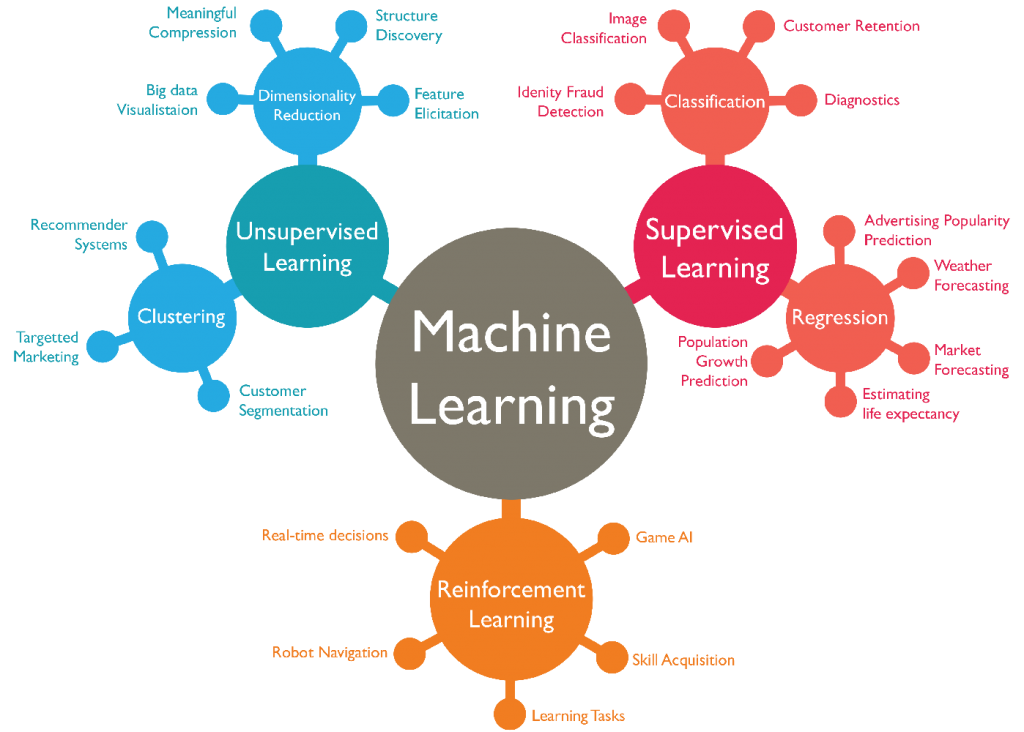
\includegraphics[width=0.9\linewidth]{tml.png}
\end{frame}


{
	\setbeamertemplate{background}{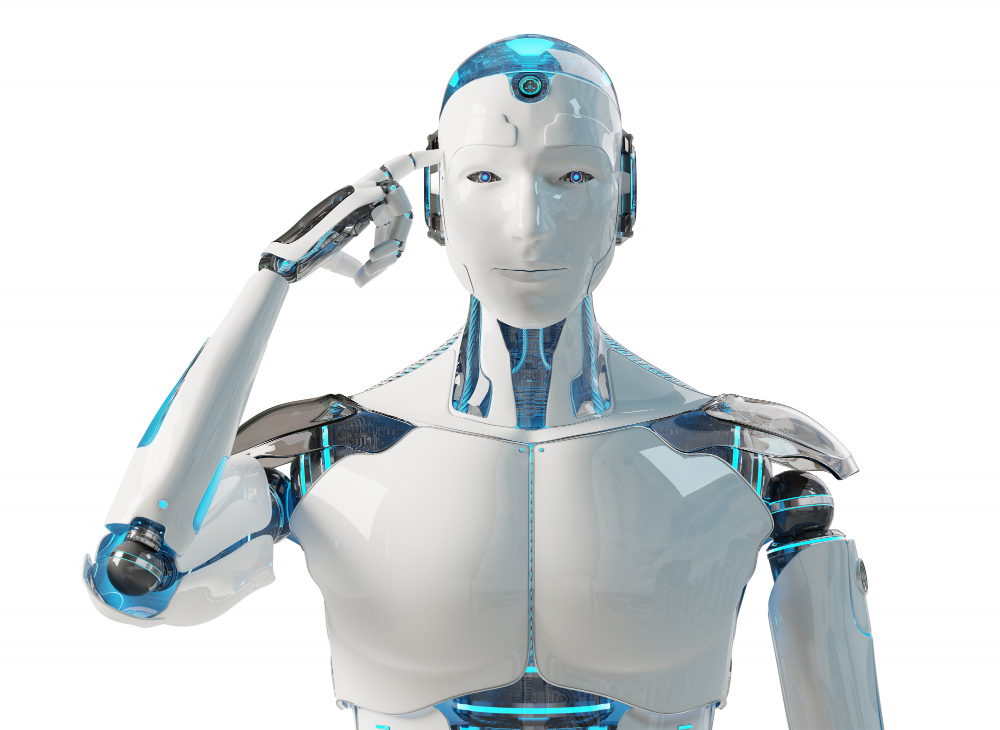
\includegraphics[width=\paperwidth,height=\paperheight]{white-male-cyborg-thinking-touching-his-head.jpg}}
\subsection{L'IA en robotique}
\begin{frame}{L'IA en robotique}
	\Large
	\begin{itemize}
		\item Applications de l'IA en robotique
		\item Exemples de robots intelligents
		\item Les défis de l'IA en robotique
	\end{itemize}
\end{frame}
}

\subsection{Applications de l'IA en robotique}
\begin{frame}{Applications de l'IA en robotique}
    \begin{itemize}
	\item Industrie : robot de gestion de chaîne d'assemblage...
	\item Armée : drone, robot-espion, robot-mule...
	\item Sécurité : vidéosurveillance...
	\item Santé : échographie, chirurgie assistée...
	\item Aérospatial : robot explorateur de la NASA...
	\item Transport : voiture autonome...
	\item Usage domestique : robot aspirateur, robot tondeuse...
	\item Accompagnement : jouet automatisé, robot humanoïde...
	\item Informatique : chatbot, assistant vocal...
\end{itemize}
\end{frame}

\begin{frame}{Exemples de Robots intelligents}
	\begin{itemize}
		\item Atlas : Robot humanoïde développé par Boston Dynamics, connu pour sa mobilité et sa dextérité avancées.
		\item Asimo : Robot humanoïde développé par Honda, célèbre pour sa marche bipède, sa capacité à monter les escaliers et ses mouvements semblables à ceux d'un humain.
		\item iCub : Robot humanoïde à source ouverte conçu pour étudier la cognition et le développement humains.
		\item Nao : Petit robot humanoïde créé par SoftBank Robotics, utilisé dans l'éducation, la recherche et le divertissement, capable d'interagir avec les humains par la parole et les gestes.
	\end{itemize}
\end{frame}

\frame[plain]
{
	\centering
	
	\movie[width=10cm,height=7.5cm,poster]{}{AtlasGetsGripBostonDynamics.mp4}
	
}
	
	
	\begin{frame}
		\frametitle{YouTube Video}
		
		\includemedia[
		width=0.6\linewidth,
		height=0.45\linewidth,
		activate=onclick,
		flashvars={
			modestbranding=1 % Hides YouTube logo
		}
		]{\strut
			\includemedia[
			activate=onclick,
			width=0.6\linewidth,
			height=0.45\linewidth,
			flashvars={
				modestbranding=1 % Hides YouTube logo
			}
			]{}{https://www.youtube.com/v/tF4DML7FIWk?rel=0}
		}{https://www.youtube.com/v/tF4DML7FIWk?rel=0}
	\end{frame}

% Slide 6: Parties prenantes
\section{Le Big Data et son intégration avec l'IA}
\subsection{Qu'est-ce que le Big Data ?}
\begin{frame}
	\frametitle{Le Big Data et son intégration avec l'IA}
	
	\begin{itemize}
		\item Les Big Data sont les traces numériques (données) qui se génèrent dans l'ensemble de l'écosystème numérique.
		\item Les Big Data sont des actifs d'information à haut volume, haute vélocité et haute variété.
		
		\item Les principales caractéristiques des Big Data sont les quatre V 
	\end{itemize}
	
	\begin{figure}
		\centering
		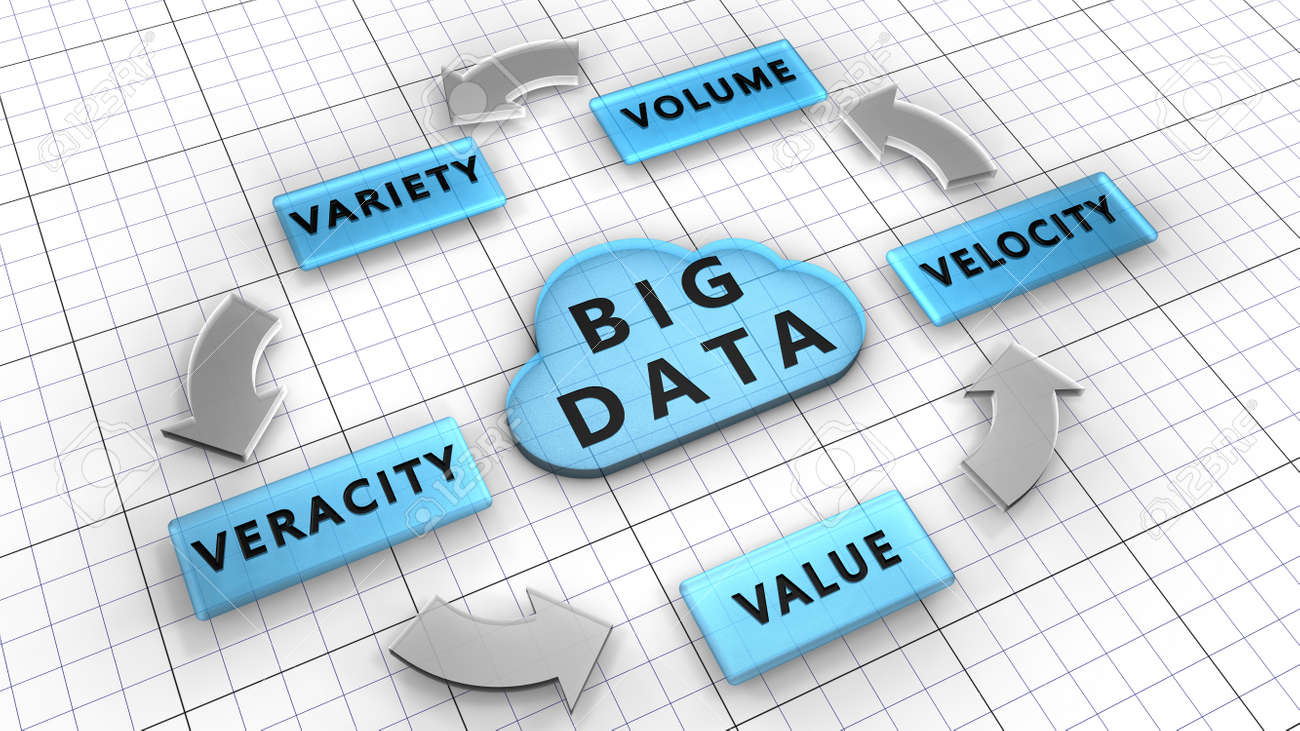
\includegraphics[width=0.6\textwidth]{bigDa.jpg}
	%	\caption{Illustration du concept de Big Data}
	\end{figure}
	
\end{frame}
\begin{comment}
		\begin{itemize}
		\item Qu'est-ce que le Big Data ?
		\item Les 4 V du Big Data (Volume, Vélocité, Variété, Véracité)
		\item Comment le Big Data alimente l'IA
	\end{itemize}
\end{comment}

\subsection{Impact des Big Data}

\begin{frame}
	\frametitle{Impact des Big Data}
	
	\begin{itemize}
		\item Les IoT génèrent continuellement d'énormes volumes de données.
\item L'analyse des Big Data aide les entreprises à obtenir des informations à partir des données collectées par les appareils IoT.
	\end{itemize}
	
	\begin{figure}
		\centering
		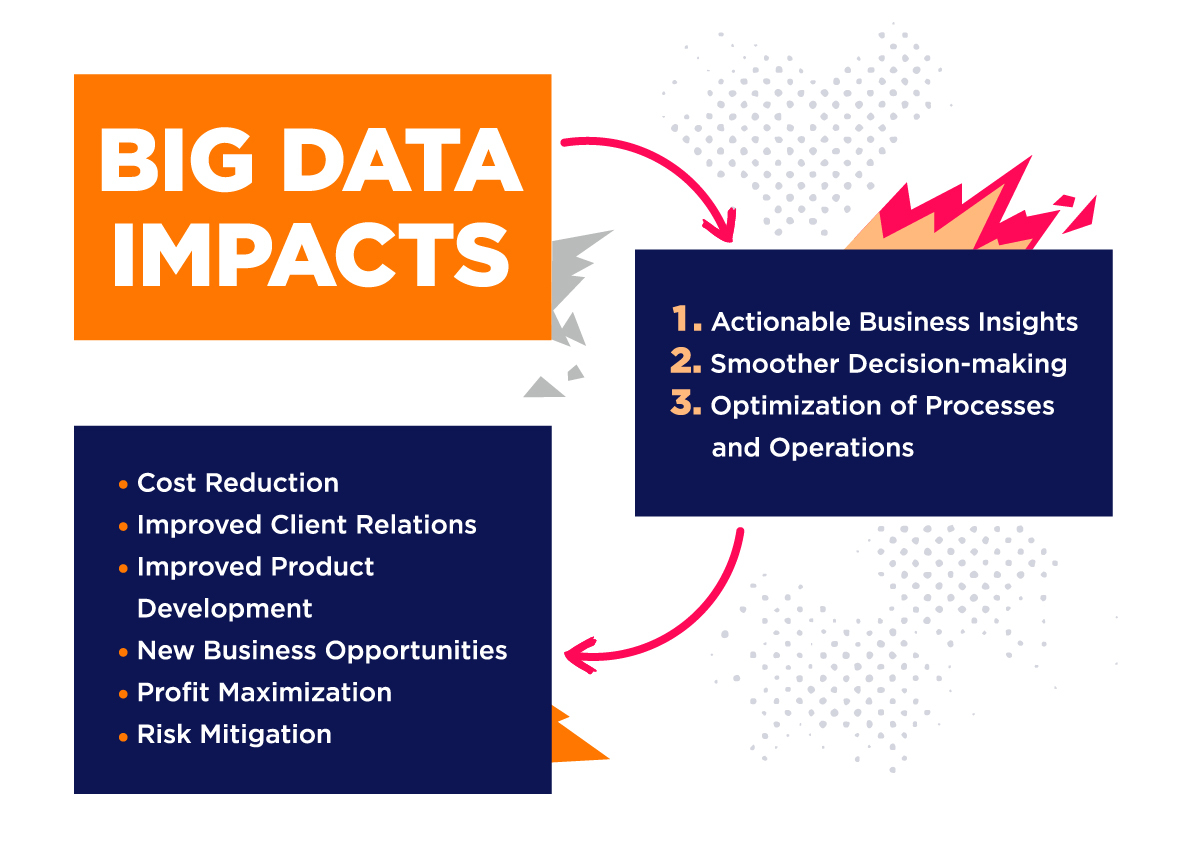
\includegraphics[width=0.6\textwidth]{big_data_benefits.jpg}
		%	\caption{Illustration du concept de Big Data}
	\end{figure}
	
\end{frame}






	\begin{frame}
	\frametitle{Comment le Big Data alimente l'IA?}
	
	\note{
	\begin{itemize}
		\item \textbf{Entraînement des modèles} :
		\begin{itemize}
			\item \textit{Fournit des ensembles de données massifs.}
			\item \textit{Permet aux modèles d'apprendre à reconnaître les relations.}
		\end{itemize}
		
		\item \textbf{Amélioration de la précision} :
		\begin{itemize}
			\item \textit{Le plus de données améliore la précision des modèles.}
			\item \textit{Diversité des sources.}
		\end{itemize}
		
		\item \textbf{Détection de tendances et de modèles cachés} :
		\begin{itemize}
			\item \textit{Analyse de grandes quantités de données.}
			\item \textit{Identifie des corrélations et des insights précieux.}
		\end{itemize}
		
		\item \textbf{Personnalisation et recommandations} :
		\begin{itemize}
			\item \textit{Analyse des préférences et des comportements des utilisateurs.}
			\item \textit{Fournit des recommandations personnalisées.}
		\end{itemize}
		
		\item \textbf{Prise de décision basée sur les données} :\textit{ informations objectives et décisions éclairées}
	\end{itemize}
}
	
		\begin{figure}
		\centering
		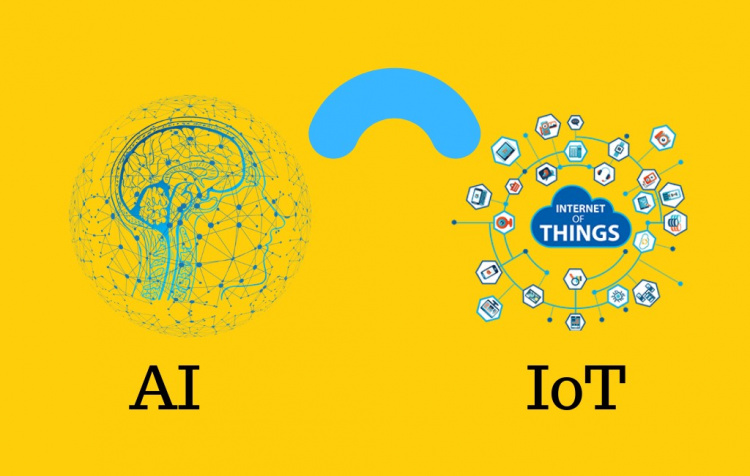
\includegraphics[width=\textwidth]{ia-capteurs-iot.jpg}
		%	\caption{Illustration du concept de Big Data}
	\end{figure}

\end{frame}



\begin{frame}
	\frametitle{Principe du Machine Learning}
	
	\begin{figure}
		\centering
		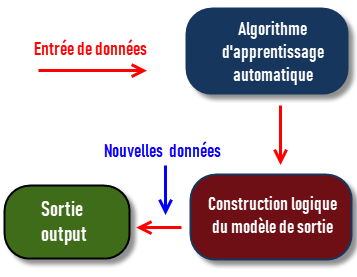
\includegraphics[width=0.7\textwidth]{ml-shema.png}
	\end{figure}

	
\end{frame}

\subsection{Les influences}
\begin{frame}{Les influences majeures du Machine Learning}
	\note{\textit{Le Machine learning ou apprentissage statistique est un champ d'étude de l'IA qui se fonde sur des approches statistiques pour donner aux ordinateurs la capacité d'apprendre à partir de données.}}
Le ML est motivé et ou soutenu par :

\begin{enumerate}
	\item La théorie formelle de la statistique
	\item L’accélération du développement des ordinateurs
	\item Le défi, dans de nombreux domaines, de corpus de données toujours plus grands
	\item L’accent mis sur la quantification dans une variété toujours plus large de disciplines
\end{enumerate}
\end{frame}

	\subsection{Méthodologie du Machine Learning}
	\begin{frame}{Comment résoudre un problème avec une approche Data?}
	\begin{figure}
			\begin{center}
			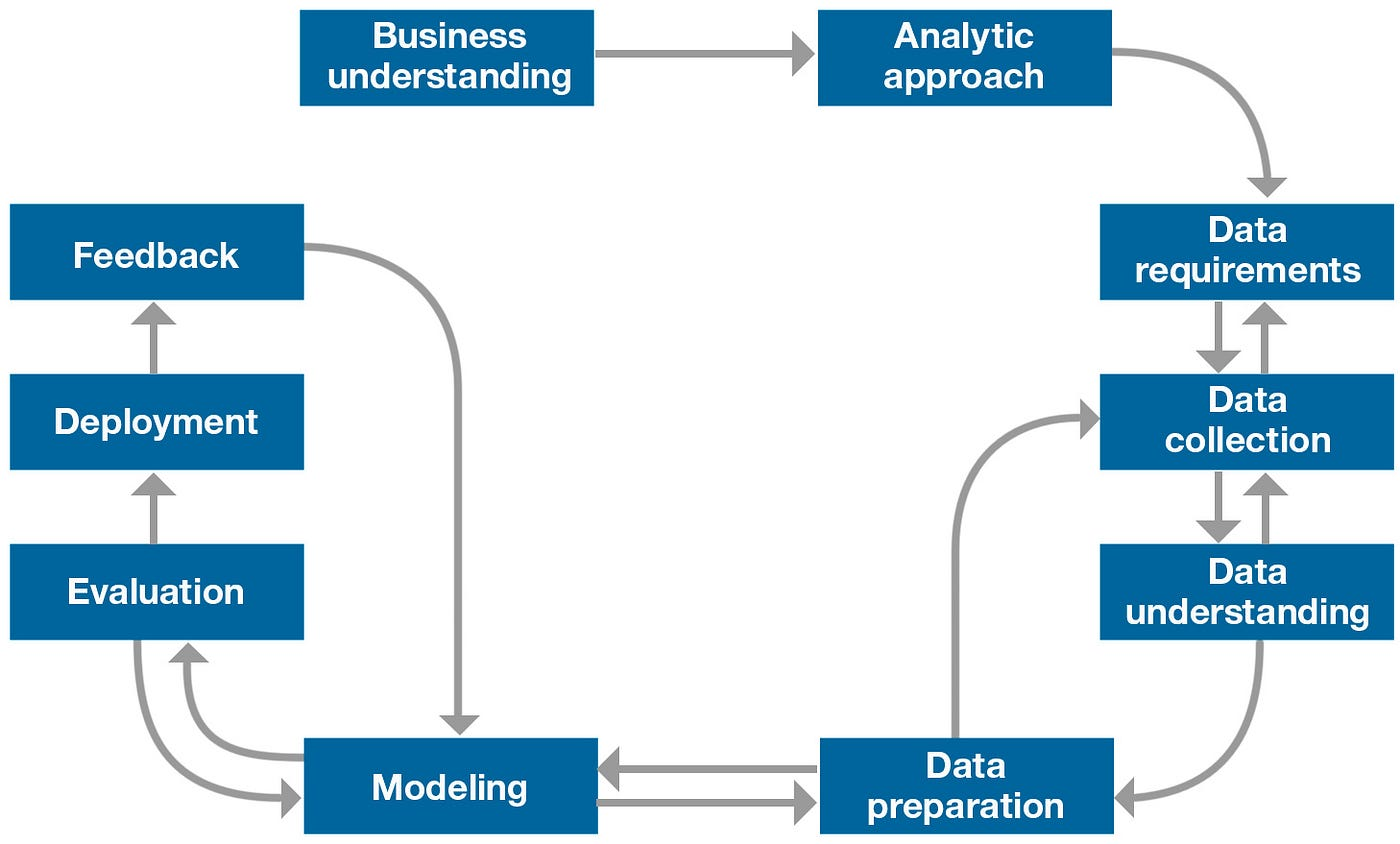
\includegraphics[scale=0.2]{DataMethod.jpg}
		\end{center}
	\caption{Data science live cycle}
	\end{figure}
	\end{frame}


	% Slide 5: Bénéfices attendus sysexpert.png




\subsection{Types d'apprentissages statistique}
\begin{frame}{Apprentissage Supervisé et non-supervisé}
\begin{itemize}
	\item Apprentissage supervisé
	\begin{itemize}
		\item Objectif : apprendre une fonction $f$ prédisant une variable $Y$ à partir de
		features $X$.
		\item Données : ensemble d'apprentissage $(X_i, Y_i)$
	\end{itemize}
 \item Apprentissage non-supervisé
 		\begin{itemize}
 			\item  Objectif: découvrir une structure au sein d'un ensemble d'individus $(X_i)$
 			\item Data : Learning set $(X_i)$
 		\end{itemize}
\end{itemize}
	\begin{figure}
	\centering
	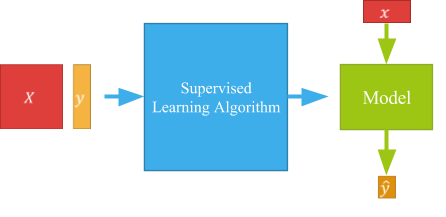
\includegraphics[width=0.6\textwidth]{Machine-Learning-3.png}
\end{figure}

\end{frame}


	\begin{frame}{Apprentissage supervisé}
	\centering
	\begin{figure}[h]
		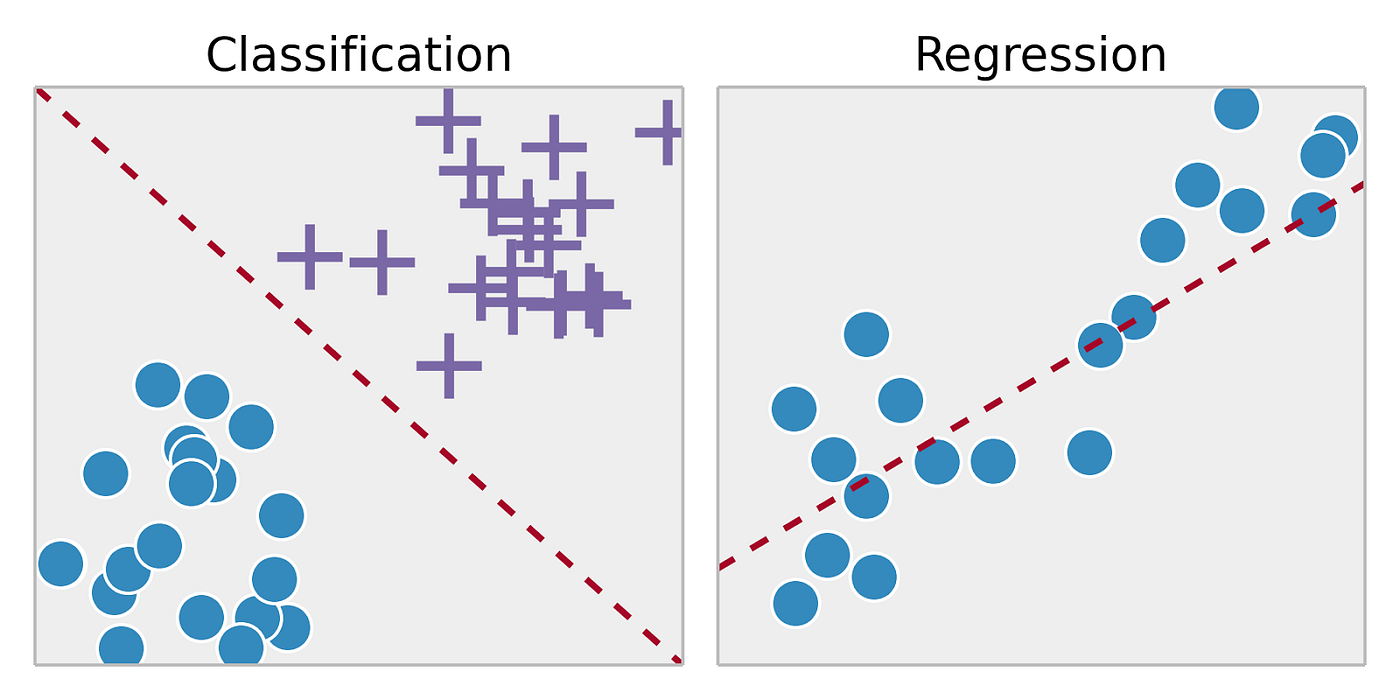
\includegraphics[width=\linewidth]{CR.png}
	%	\caption{Classification Vs Regression}
	\end{figure}
\end{frame}	



%	\setbeamertemplate{background}{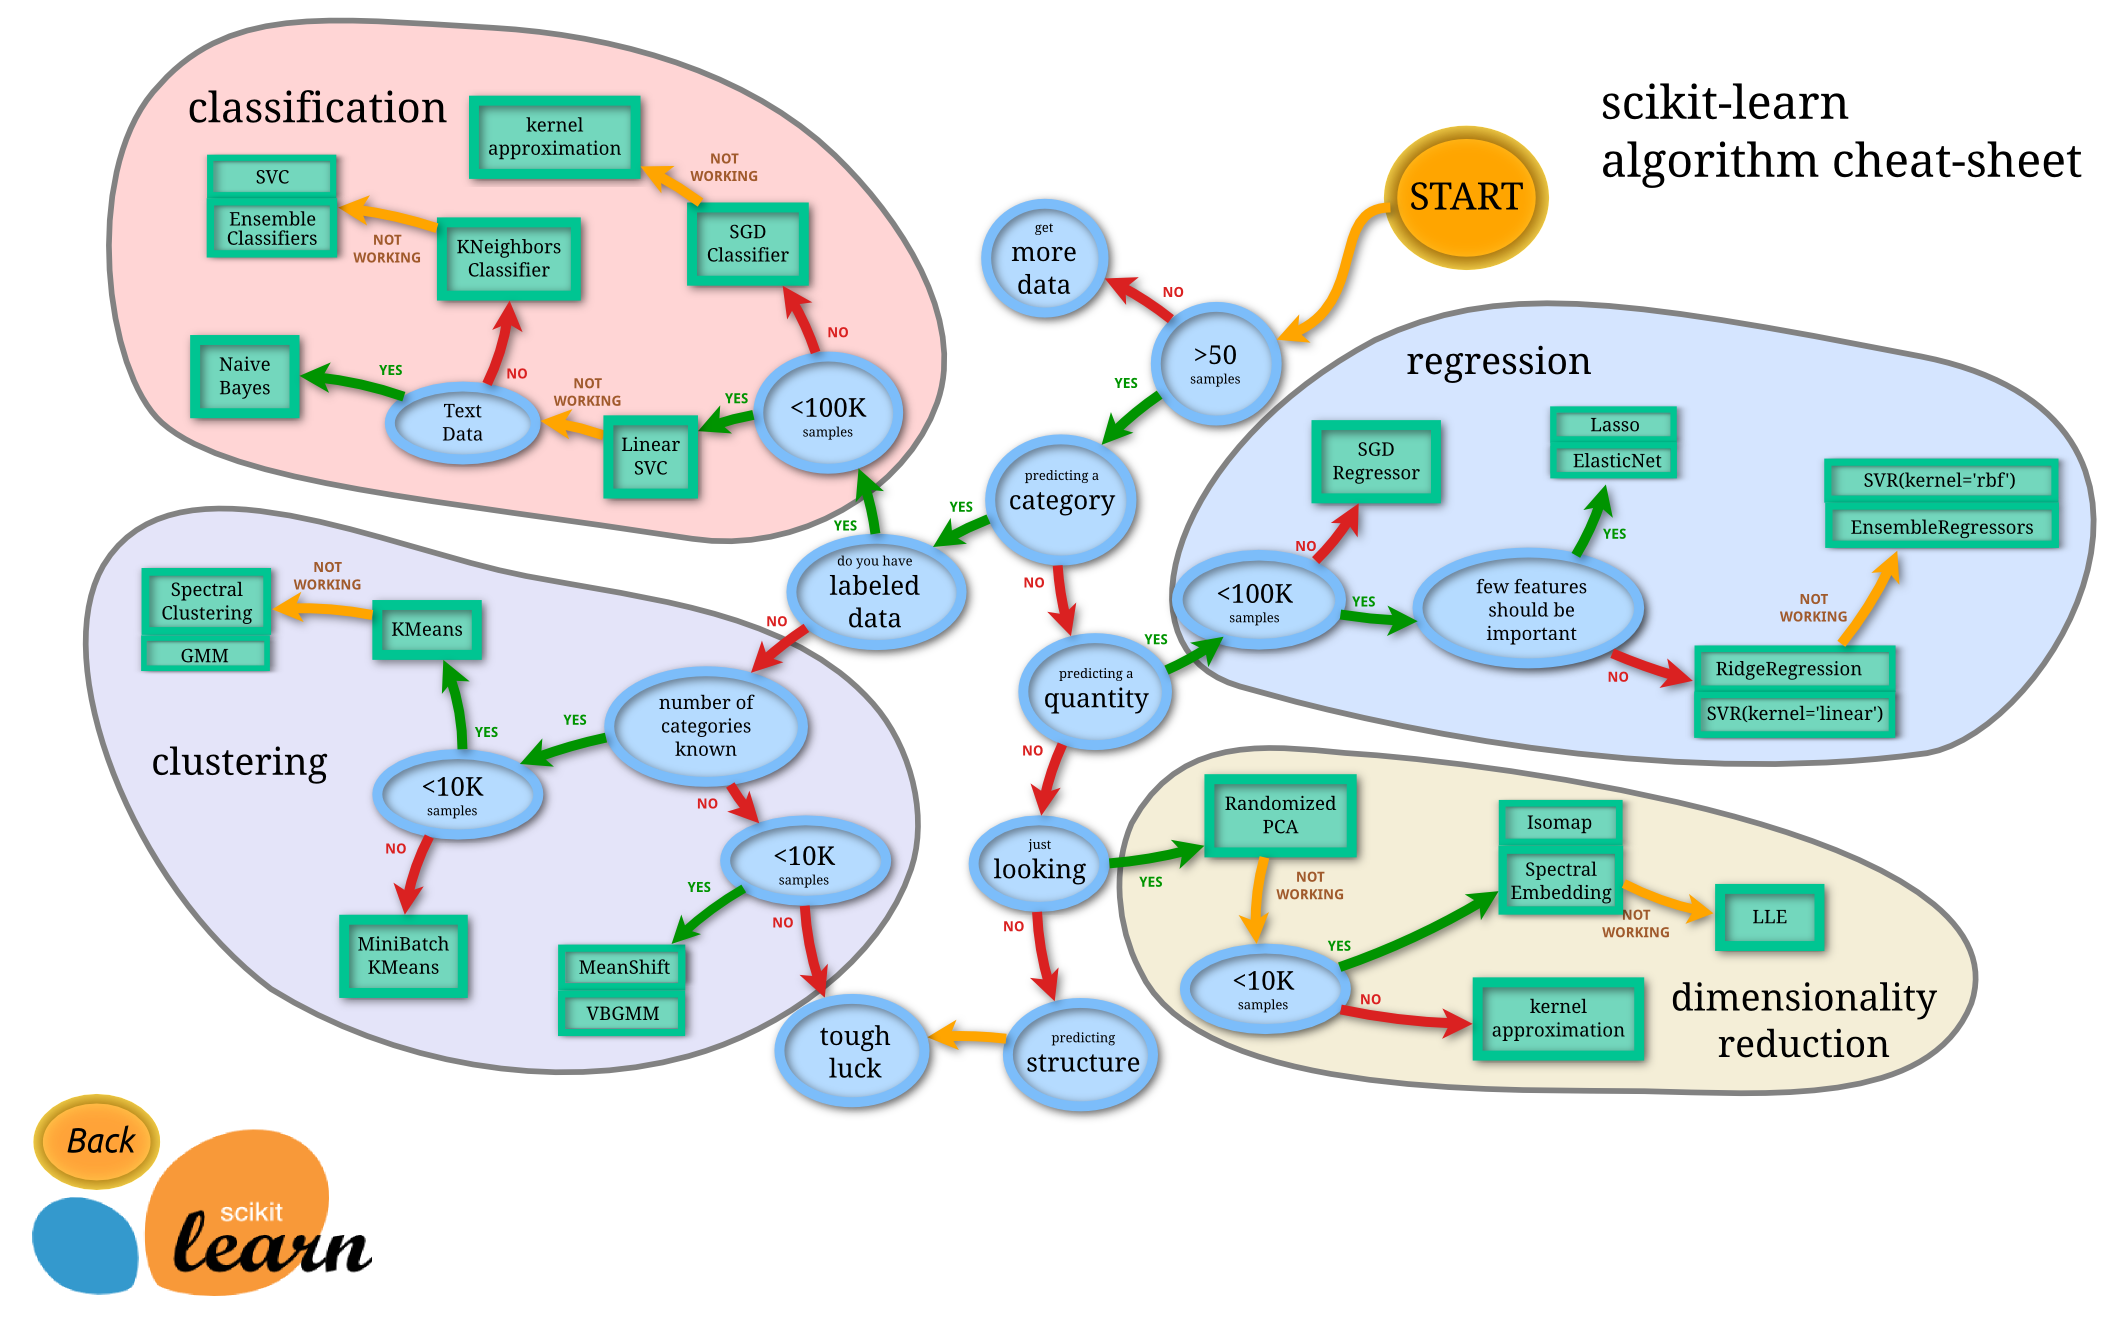
\includegraphics[width=\paperwidth,height=\paperheight]{ml_map.png}}


\subsection{Types de Machine Learning - Quiz}
	\begin{frame}
	\frametitle{Quiz: Classification ou Regression?}
	\note{
		\begin{itemize}
			\item[1-] \textit{Il s'agit d'un problème de régression, car l'objectif est de prédire une valeur numérique continue dans le future.}
\item[2-]\textit{ Détection de piratage ou de compromission des comptes : C'est un problème de classification. La réponse est binaire, c'est-à-dire qu'elle peut être catégorisée en deux classes distinctes.}

\item[3-] \textit{Prédiction du churn (taux de désabonnement) d'une entreprise : C'est un problème de classification, car l'objectif est de prédire si un client donnera son avis positif ou négatif} 

\item[4-] \textit{Prédiction de conversion d'un prospect en client : C'est un problème de classification, car il s'agit de prédire si un prospect deviendra un client ou non. La réponse est binaire: conversion ou non conversion.}

\item[5-] \textit{Prédiction du chiffre d'affaires d'une entreprise dans 10 ans : Il s'agit d'un problème de régression, car l'objectif est de prédire une valeur numérique continue pour une période de temps spécifique.}
\end{itemize}
}
\begin{itemize}
	\item[1-]  Vous avez un large inventaire d'articles identiques. Vous voulez prédire
	combien de ces articles se vendront au cours des 3 prochains mois.
	\item[2-]  Vous devez examiner les comptes de vos clients et décider pour chacun d’entre eux s'ils ont été piratés ou compromis. 
	\item[3-] Prédiction du churn d'une entreprise
	\item[4-] Prédire si un prospect deviendra client
	\item[5-] Prédire le chiffre d'affaire d'une entreprise dans 10 ans
\end{itemize}	
\end{frame}		
	
\begin{frame}
	\frametitle{Exercise : Study case}
	
	\begin{center}
		\textbf{Given a case study: pricing apartments based on a real estate website.}
	\end{center}
	
	\vspace{0.5cm}
	
	\begin{itemize}
		\item House descriptions with their price
		\item Predicting house prices from their description
		\item Use case: finding houses that are cheap compared to market value
	\end{itemize}
	
\end{frame}

\begin{frame}
	\frametitle{Question 1}
	\note{
	\begin{itemize}
		\item[a)] \textit{It's a supervised learning problem because we have houses description and for each of them we have the corresponding price.}
		\item[d)] \textit{It's a regression problem because the value that we're trying to predict (price) is a continue value.}
	\end{itemize}
}
	\textbf{What kind of problem is it?}
	
	\begin{enumerate}
		\item[a)] A supervised problem
		\item[b)] An unsupervised problem
		\item[c)] A classification problem
		\item[d)] A regression problem
	\end{enumerate}
	
	\vspace{0.5cm}
	
	\textbf{Select all answers that apply}
	
\end{frame}

\begin{frame}
	\frametitle{Question 2}
	\note{
	\begin{itemize}
		\item[a)] \textit{To know the features, ask you the question "What is pertinent to explain the house price?". In this case it's the number of rooms.}
		\item[b)] \textit{The post code of the house is also important because it provides geographic informations.}
	\end{itemize}
}
	\textbf{What are the features?}
	
	\begin{enumerate}
		\item[a)] The number of rooms might be a feature
		\item[b)] The post code of the house might be a feature
		\item[c)] The price of the house might be a feature
	\end{enumerate}
	
	\vspace{0.5cm}
	
	\textbf{Select all answers that apply}
	
\end{frame}

\begin{frame}
	\frametitle{Question 3}
	\note{
	\begin{enumerate}
	\item[b)] \textit{The price of the house is the target. It's the variable that we're trying to predict.}
	\item[c)] \textit{House descriptions with no price mentioned are the set of independant variable (features) generally assign in a matrix} $X$.
\end{enumerate}	
}
	\textbf{What is the target variable?}
	
	\begin{enumerate}
		\item[a)] The full text description is the target
		\item[b)] The price of the house is the target
		\item[c)] Only house descriptions with no price mentioned are the target
	\end{enumerate}
	
	\vspace{0.5cm}
	
	\textbf{Select a single answer}
	
\end{frame}

\begin{frame}
	\frametitle{Question 4}
	\note{
	\begin{enumerate}
	\item[a)] \textit{Each house description is a record, only.}
\end{enumerate}	
}
	
	\textbf{What is a record (a sample, instance)?} (observation)
	
	\begin{enumerate}
		\item[a)] Each house description is a record
		\item[b)] Each house price is a record
		\item[c)] Each kind of description (e.g., house size) is a record
	\end{enumerate}
	
	\vspace{0.5cm}
	
	\textbf{Select a single answer}
	
\end{frame}
	

	
	\begin{frame}{Apprentissage non-supervisé (clustering)}
		
		\note{
	\begin{itemize}
		\item \textit{Le clustering est une technique d'apprentissage non supervisé qui regroupe des données similaires en ensembles distincts appelés clusters. Il aide à découvrir des structures et des relations inhérentes aux données sans avoir d'étiquettes prédéfinies.}
		\item \textit{ Imaginons que nous ayons un ensemble de données contenant des informations sur des clients d'un site de commerce électronique, comme leur âge, leur revenu, et leurs habitudes d'achat. Nous pourrions utiliser le clustering pour regrouper ces clients en segments homogènes en fonction de leurs caractéristiques similaires.  Nous pourrions obtenir différents clusters représentant des profils de clients distincts. Par exemple, nous pourrions identifier un cluster de \textbf{jeunes consommateurs à faible revenu}, un autre cluster de \textbf{clients aisés et fréquents}, et un troisième cluster de \textbf{clients plus âgés et prudents}.} 
	\end{itemize}	
	}
			\begin{columns}
				\begin{column}{0.5\textwidth}
					\centering
					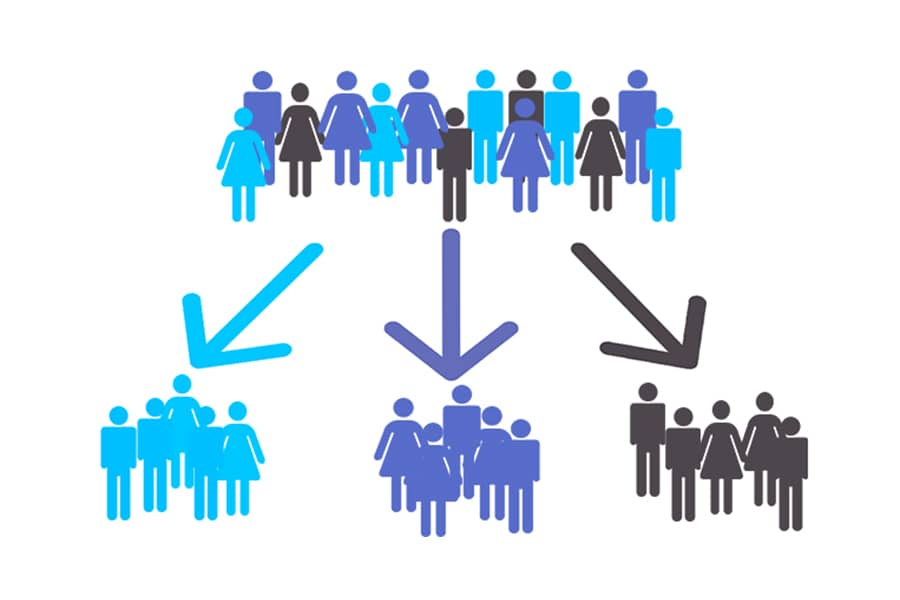
\includegraphics[width=\textwidth]{segmentation.jpg}
					\par
				$3$ Clusters constitués à partir d'un dataset hétérogène
				\end{column}
				
				\begin{column}{0.5\textwidth}
					\centering
					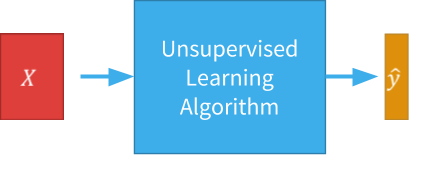
\includegraphics[width=\textwidth]{Machine-Learning-9.png}
					\par
					Principe du clustering
				\end{column}
			\end{columns}
	\end{frame}
	% Slide 8: Conception conceptuelle
		\begin{frame}{Reduction de la dimension}
			\note{
			\begin{itemize}
				
				\item \textit{Les plateformes comme Netflix utilise la réduction de la dimensionnalité, notamment la factorisation matricielle, pour recommander des films en se basant sur ceux que vous avez déjà visionnés.}
				\item  \textit{Cette technique permet de représenter les films et les utilisateurs dans un espace de dimensions réduites, où les similarités peuvent être calculées plus efficacement. En utilisant ces représentations réduites, Netflix peut recommander des films similaires à ceux que vous avez aimés.}
			\end{itemize}
		}
		\centering
		\begin{figure}[h]
			
\includegraphics[width=0.95\linewidth]{Net.png}
			\caption{Recommendation}
		\end{figure}
	\end{frame}



\begin{frame}{Réduction de la Dimensionnalité}
	\begin{itemize}
		\item Technique utilisée pour réduire le nombre de features d'un dataset.
		\item Objectifs de la réduction de la dimensionnalité :
		\begin{itemize}
			\item Réduire la complexité du modèle et le temps de calcul.
			\item Éliminer les redondances et le bruit dans les données.
			\item Visualiser les données dans un espace de dimension inférieure.
		\end{itemize}
		\item Méthodes courantes de réduction de la dimensionnalité :
		\begin{itemize}
			\item Analyse en composantes principales (PCA) : transforme les variables d'origine en un nouvel ensemble de variables non corrélées appelées CP.
			\item Sélection de caractéristiques : sélectionne un sous-ensemble de caractéristiques les plus informatives.
			\item Manifold Learning : trouve des représentations non linéaires des données dans un espace de dimension inférieure.
		\end{itemize}
	\end{itemize}
\end{frame}


	\begin{frame}{Scikit Learn : famous ML library}
\note{		\begin{itemize}
			\item \textit{Scikit-learn : bibliothèque open-source pour l'apprentissage automatique en Python.}
			\item \textit{Large gamme d'outils et d'algorithmes pour la classification, la régression, le clustering, etc.}
			\item \textit{Prise en charge des tâches de prétraitement de données, de sélection de modèles, etc.}
				\item \textit{Régression linéaire : modélisation des relations linéaires entre les variables.}
				\item \textit{SVM (Support Vector Machines) : classification et régression basées sur la recherche de la meilleure séparation entre les classes.}
			
		\end{itemize}}
	\centering
	\begin{figure}[h]
		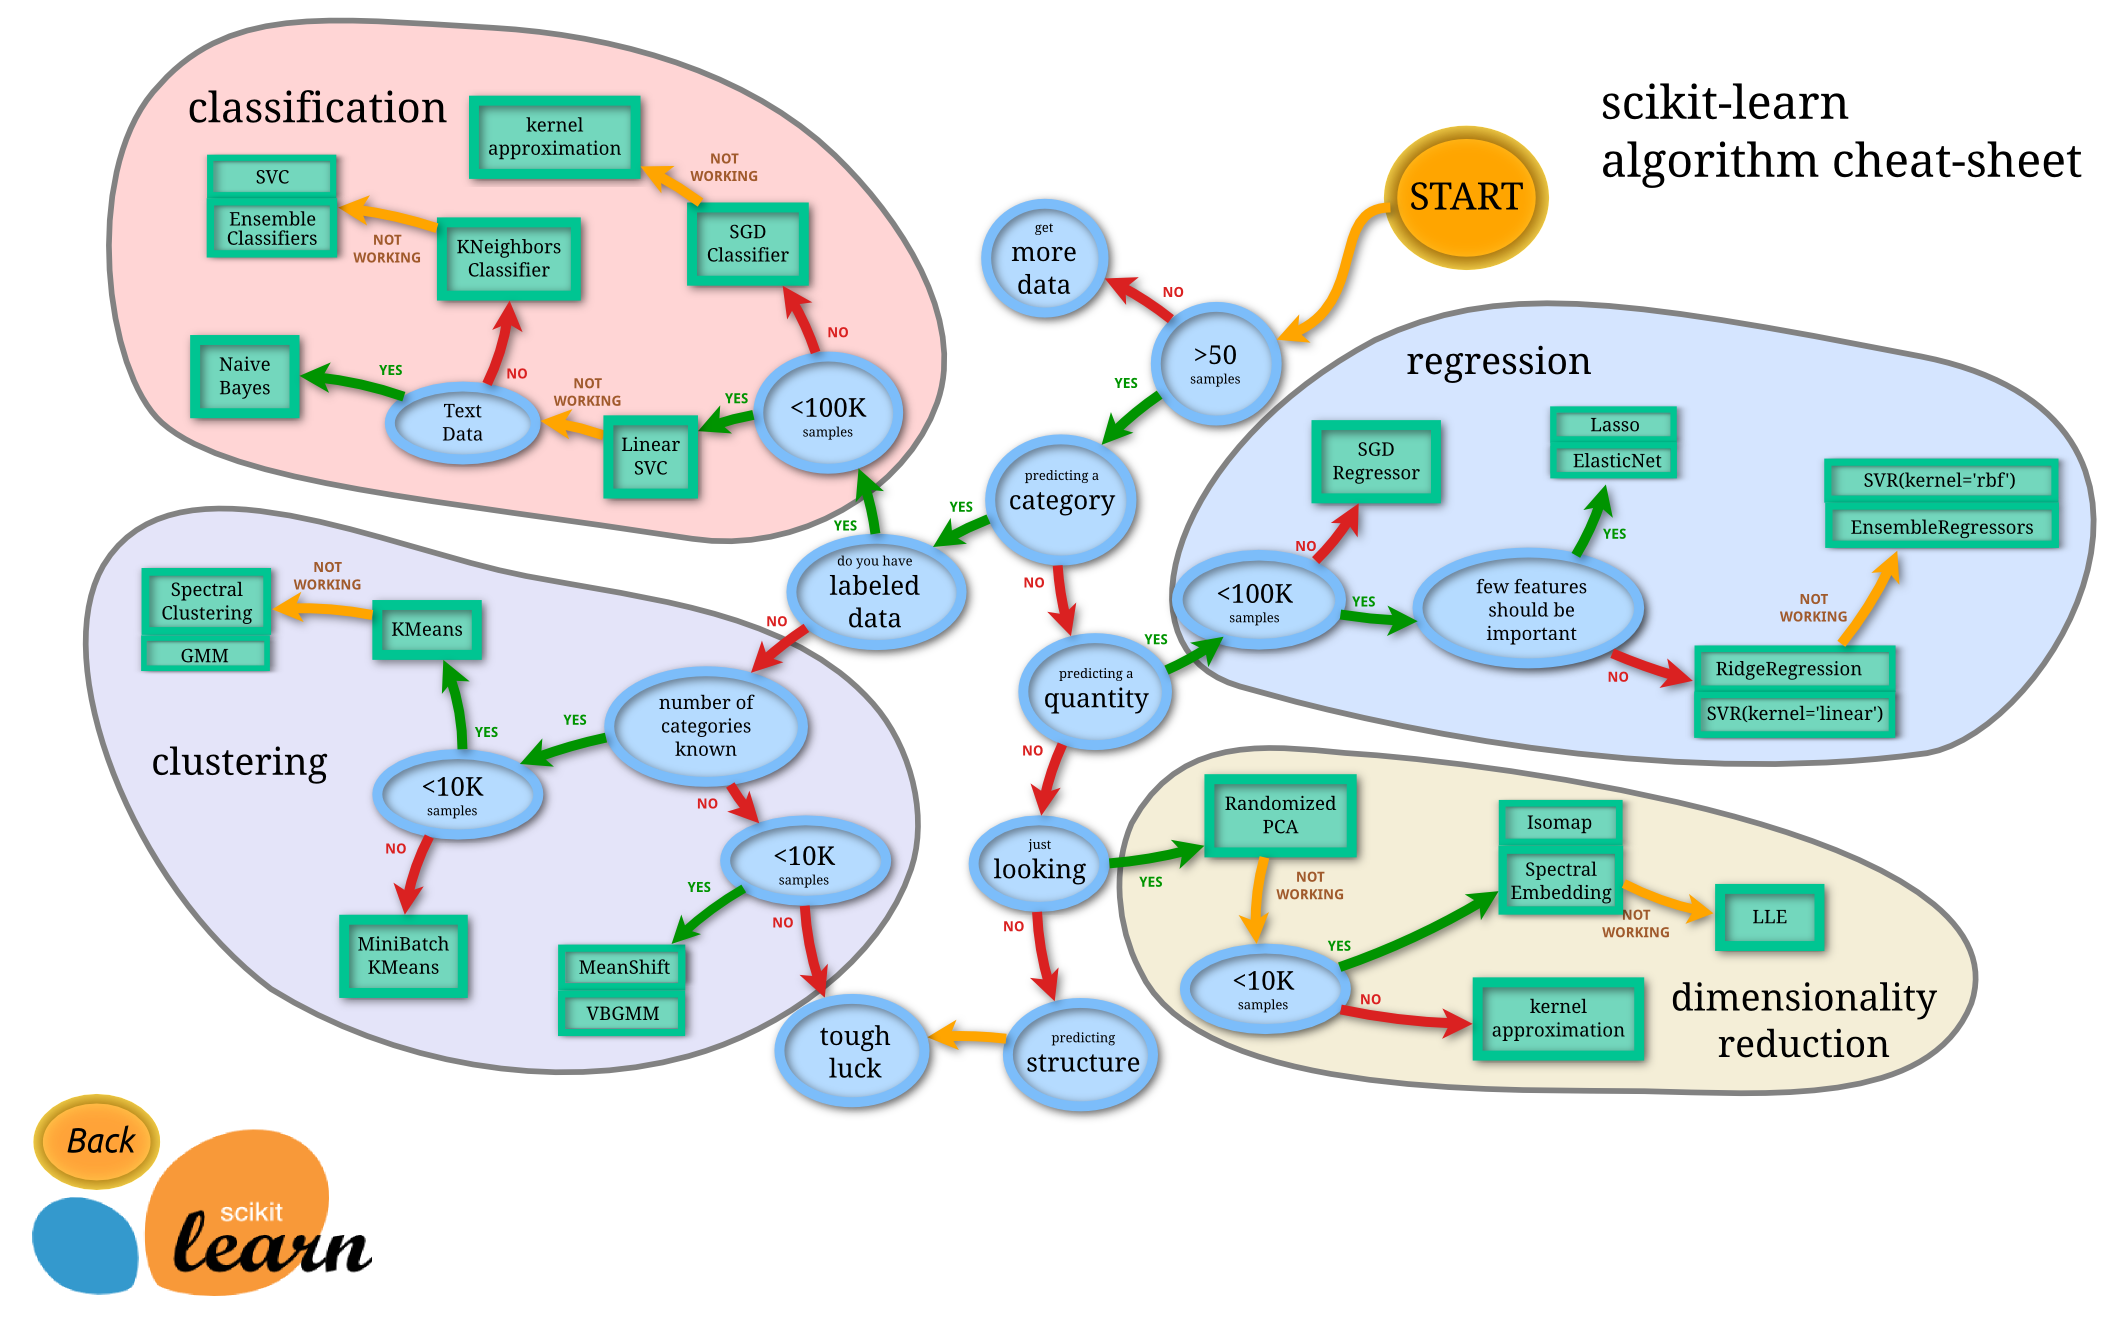
\includegraphics[width=\linewidth]{ml_map.png}
		\caption{Grand catalogue de méthodes de ML}
	\end{figure}
\end{frame}
	% Slide 9: Conclusion
	\subsection{Eviter les pièges en Machine Learning}
\begin{frame}{Travailler avec les données et éviter les pièges}
	\framesubtitle{Collecte et préparation des données}
	\begin{enumerate}
		\item Collecte des données de qualité et représentatives
			\begin{itemize}
				\item Déterminez les informations que vous voulez collecter
				\item Définissez la méthode de collecte des données
			\end{itemize}
		\item Exploration des données (Data mining)
			\begin{itemize}
				\item Compréhension du problème (activité, objectif)
				\item Compréhension des données
			\end{itemize}
		\item Nettoyage des données 
			\begin{itemize}
				\item Gestion des erreurs de saisie
				\item  Gestion des doublons
				\item  Gestion des valeurs manquantes et des données aberrantes
			\end{itemize}
		\item Les bonnes pratiques de normalisation et transformation des données
	\end{enumerate}
\end{frame}
	
	% Slide 10: Contac
	
\begin{frame}{Travailler avec les données et éviter les pièges}
	\framesubtitle{Sélection des caractéristiques et modélisation}
	\begin{enumerate}
		\item Feature selection (features pertinentes pour le modèle)
		\item Choix et évaluation des modèles
			\begin{itemize}
				\item Sélection du modèle approprié en fonction du problème et des data
				\item L'utilisation de la validation croisée pour évaluer le modèle
				\item L'interprétation des métriques d'évaluation telles que la précision, le rappel, le F1-score, etc.
			\end{itemize}
		\item Gestion du déséquilibre des classes 
		   \begin{itemize}
		   	\item L'identification et la gestion du déséquilibre des classes dans les problèmes de classification
		    \item 	L'utilisation de techniques de suréchantillonnage, de sous-échantillonnage ou d'ajustement des poids des classes pour traiter ce déséquilibre
		   \end{itemize}
		%Réduction du surajustement (overfitting)
			
	\end{enumerate}
\end{frame}


		\begin{frame}{Travailler avec les données et éviter les pièges}
\note{\begin{itemize}
		\item Overfitting (Surapprentissage) en régression :
		\begin{itemize}
			\item Modèle trop complexe par rapport au training set.
			\item Excellente performance sur le trainset, mais mauvaise sur de nouvelles données.
			\item Le modèle "mémorise" les données d'entraînement spécifiques au lieu de généraliser les tendances sous-jacentes.
			\item Peut se produire lorsque le modèle a un nombre excessif de paramètres par rapport à la taille des données d'entraînement.
		\end{itemize}
		
		\item Underfitting (Sous-apprentissage) en régression :
		\begin{itemize}
			\item Le modèle est trop simple pour capturer les tendances sous-jacentes des données.
			\item Performance médiocre à la fois sur les train et new data.
			\item Le modèle ne parvient pas à saisir les relations complexes entre les variables.
			\item Peut se produire lorsque le modèle est trop limité en termes de capacité ou que le trainset insuffisantes.
		\end{itemize}
\end{itemize}}
	
	\centering
	\begin{figure}[h]
		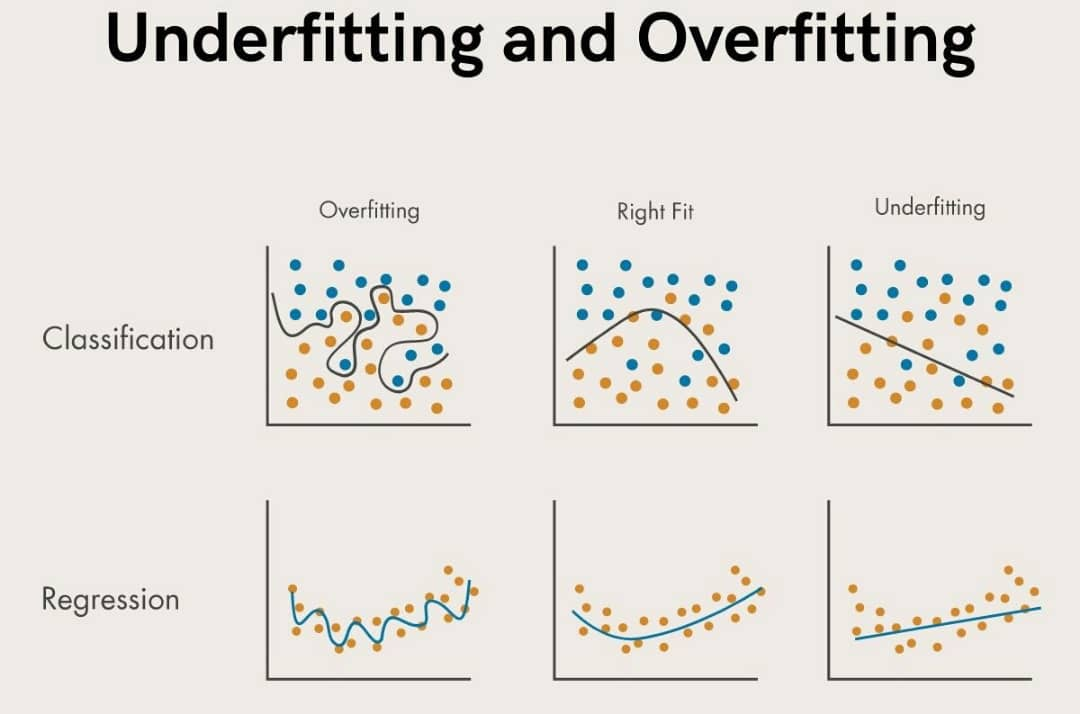
\includegraphics[width=0.87\linewidth]{OverUnderFit.jpeg}
		%\caption{Recommendation}
	\end{figure}

\end{frame}

\begin{frame}{Travailler avec les données et éviter les pièges}
\framesubtitle{Gestion de l'Overfitting et de l'Underfitting en régression}

\note{ \textbf{Gestion de l'overfitting en régression :}

	\begin{itemize}
		\item \textit{Utiliser des techniques de régularisation telles que la régression ridge ou la régression Lasso pour limiter la complexité du modèle.}
		\item \textit{Collecter davantage de données d'entraînement pour fournir une meilleure représentation de la variabilité des données réelles.}
		\item \textit{Utiliser la validation croisée pour évaluer la performance du modèle.}
	\end{itemize}
	
 \textbf{Gestion de l'underfitting en régression :}
	\begin{itemize}
		\item \textit{Utiliser un modèle plus complexe comme une régression polynomiale pour capturer des relations non linéaires entre les variables.}
		\item \textit{Ajouter de nouvelles caractéristiques ou transformer les caractéristiques existantes pour fournir plus d'informations.}
		\item \textit{Augmenter la capacité du modèle en augmentant le nombre de paramètres ou de couches dans un réseau de neurones.}
	\end{itemize}
}

	\begin{itemize}
		\item \textbf{Overfitting} : Réduire la complexité du modèle, utiliser la régularisation et la validation croisée.
		\item \textbf{Underfitting} : Augmenter la complexité du modèle et ajouter de nouvelles caractéristiques.
	\end{itemize}
		\centering
\begin{figure}[h]
	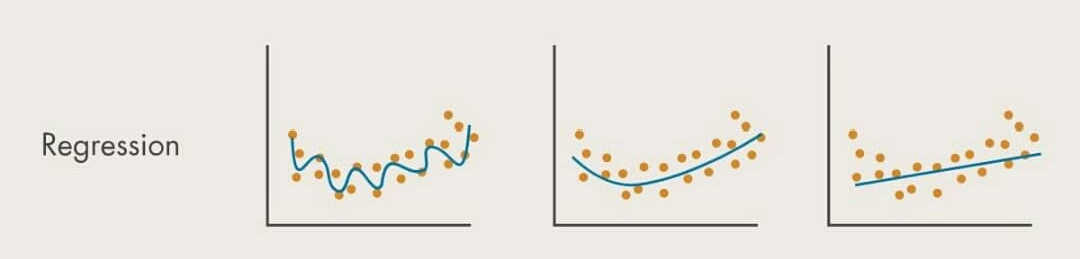
\includegraphics[width=0.93\linewidth]{OverUnderFitRegression.jpeg}
\end{figure}
\end{frame}

\begin{frame}{Travailler avec les données et éviter les pièges}
	\framesubtitle{Gestion de l'Overfitting et de l'Underfitting en classification}
	\note{\begin{itemize}
			\item Gestion de l'overfitting en classification :
			\begin{itemize}
				\item \textit{Utiliser des techniques de régularisation comme la pénalisation L1 ou L2 pour réduire la complexité du modèle.}
				\item \textit{Appliquer des techniques de réduction de dimensionnalité pour sélectionner les caractéristiques les plus informatives.}
				\item \textit{Utiliser l'augmentation de données pour augmenter la taille et la diversité de l'ensemble d'entraînement.}
			\end{itemize}
			
			\item Gestion de l'underfitting en classification :
			\begin{itemize}
				\item \textit{Utiliser un modèle plus complexe comme les machines à vecteurs de support (SVM) non linéaires ou les réseaux de neurones profonds.}
				\item \textit{Ajouter des caractéristiques supplémentaires ou des transformations des caractéristiques existantes pour améliorer la représentation des données.}
				\item \textit{Ajuster les paramètres du modèle pour augmenter sa capacité et permettre une meilleure adaptation aux données.}
			\end{itemize}
	\end{itemize}}

	\begin{itemize}
		\item \textbf{Overfitting} : Utiliser la régularisation, la validation croisée et l'ajustement des hyperparamètres pour limiter la complexité du modèle.
		\item \textbf{Underfitting} : Augmenter la complexité du modèle en ajoutant de nouvelles caractéristiques ou en utilisant des modèles plus sophistiqués.
	\end{itemize}

		\centering
\begin{figure}[h]
	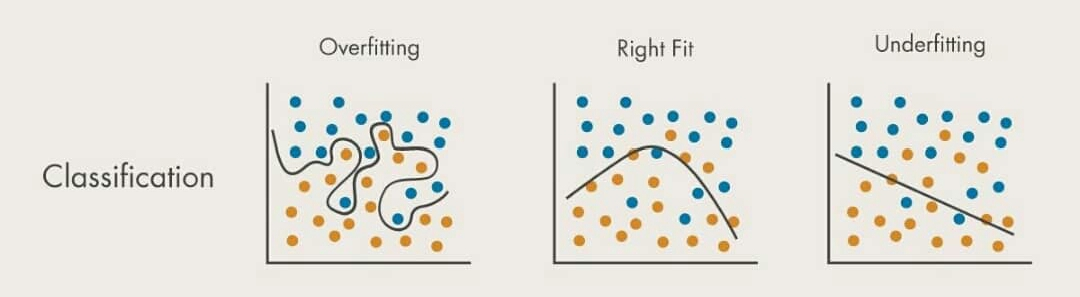
\includegraphics[width=0.93\linewidth]{OverUnderFitClasssification.jpeg}
\end{figure}
\end{frame}
% Jour 2
\subsection{Quelques modèles de ML}
\begin{frame}{Quelques modèles de Machine Learning}
	\note{
\begin{itemize}
	\item \textbf{Source de connaissances :}
	\begin{itemize}
		\item Humain : \textit{expérience, observation, interaction avec l'environnement.}
		\item Machine : \textit{algorithmes et modèles statistiques apprenant à partir de données.}
	\end{itemize}
	
	\item \textbf{Capacité d'abstraction :}
	\begin{itemize}
		\item Humain : \textit{capacité naturelle à généraliser et à appliquer des connaissances à de nouvelles situations.}
		\item Machine : \textit{nécessite souvent un grand nombre de données étiquetées pour généraliser.}
	\end{itemize}
	
	\item \textbf{Adaptabilité et flexibilité :}
	\begin{itemize}
		\item Humain : \textit{capacité à apprendre de nouvelles tâches avec peu d'exemples.}
		\item Machine : \textit{nécessite un entraînement spécifique pour chaque tâche et peut avoir du mal à se généraliser.}
	\end{itemize}
	
	\item \textbf{Explicabilité :}
	\begin{itemize}
		\item Humain : \textit{capacité à expliquer le raisonnement et les décisions.}
		\item Machine : \textit{certains modèles sont difficiles à interpréter.}
	\end{itemize}
\end{itemize}	
}
	\begin{center}
		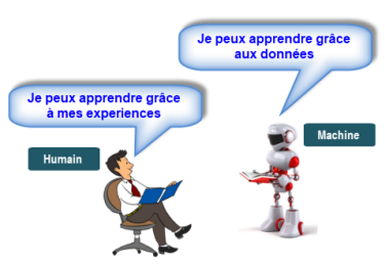
\includegraphics[scale=0.8]{machineLearning.png}
	\end{center}
\end{frame}

\begin{comment}
	\begin{frame}
	\frametitle{Sélection de l'algorithme approprié}
	\begin{itemize}
		\item Importance de choisir le bon algorithme en fonction du problème et des données
		\item Considérations sur la capacité de généralisation, la complexité et l'interprétabilité des modèles
	\end{itemize}
\end{frame}
\end{comment}


\begin{frame}{Modèles de Régression}
	\note{        
		\textbf{Régression Linéaire}:
		La régression linéaire modélise la relation entre les variables explicatives et la variable cible à l'aide d'une équation linéaire. Par exemple, on peut utiliser la régression linéaire pour prédire le prix d'une maison en fonction de sa superficie, du nombre de chambres, de l'année de construction, etc.
		
		\textbf{Régression Logistique}:
		La régression logistique estime la probabilité qu'une variable dépendante binaire (0 ou 1) prenne la valeur 1 en fonction des variables explicatives. Par exemple, on peut utiliser la régression logistique pour prédire la probabilité qu'un client achète un produit en fonction de son âge, de son revenu, de ses intérêts, etc.}
	\textbf{Régression Linéaire}
	
	\vspace{0.5cm}
	
	Modélisation: relation entre les variables explicatives et la variable cible

	\[
	y = \beta_0 + \beta_1x_1 + \beta_2x_2 + \ldots + \beta_nx_n + \epsilon
	\]
	
	\begin{itemize}
		\item $y$ : Variable dépendante à prédire
		\item $x_1, x_2, \ldots, x_n$ : Variables indépendantes (caractéristiques)
		\item $\beta_0, \beta_1, \beta_2, \ldots, \beta_n$ : Coefficients de régression à estimer
		\item $\epsilon$ : Terme d'erreur aléatoire
	\end{itemize}
	
	\vspace{0.5cm}
	
	\textbf{Régression Logistique}
	\[
	P(y=1) = \frac{1}{1 + e^{-(\beta_0 + \beta_1x_1 + \beta_2x_2 + \ldots + \beta_nx_n)}}
	\]
	
	\begin{itemize}
		\item $P(y=1)$ : Probabilité que la variable dépendante $y$ prenne la valeur 1
		\item $x_1, x_2, \ldots, x_n$ : features.
	\end{itemize}
	
\end{frame}


\begin{frame}{Arbre de Décision}
	\note{\note{
			L'arbre de décision est un modèle qui utilise une structure en forme d'arbre pour prendre des décisions ou faire des prédictions. Il est construit en partitionnant les données en fonction des caractéristiques jusqu'à une condition d'arrêt. Il est interprétable et sensible aux variations des données d'entraînement.
	}}
	\begin{itemize}
		\item Modèle d'apprentissage automatique non linéaire et non paramétrique
		\item Représente une série de décisions basées sur les features
		\item Utilisé pour la classification et la régression
	\end{itemize}
	
	\begin{center}
		\begin{figure}
	%	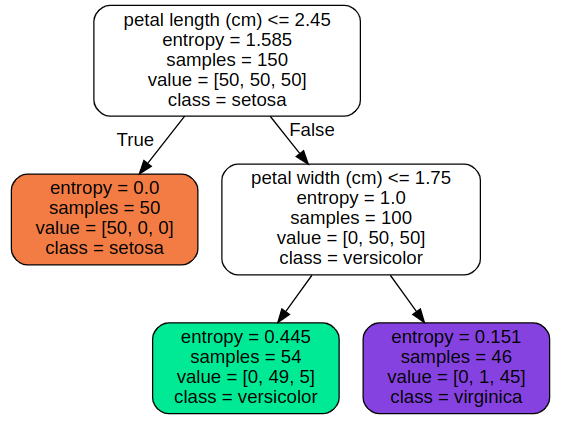
\includegraphics[width=0.6\textwidth]{iris.png}
		    \begin{minipage}[t]{0.45\linewidth}
			\centering
			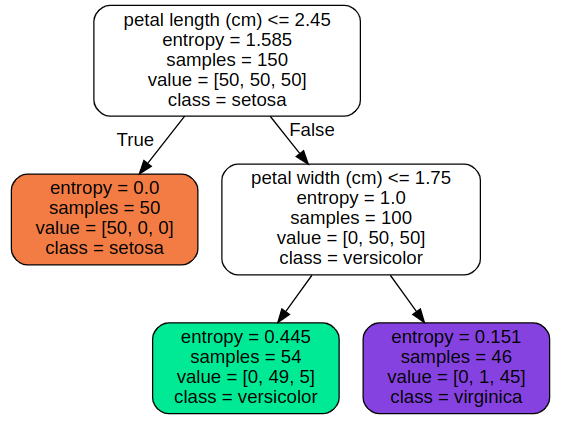
\includegraphics[width=\linewidth]{iris.png}
			\caption{Classification tree}
		\end{minipage}
		\hfill
		\begin{minipage}[t]{0.45\linewidth}
			\centering
			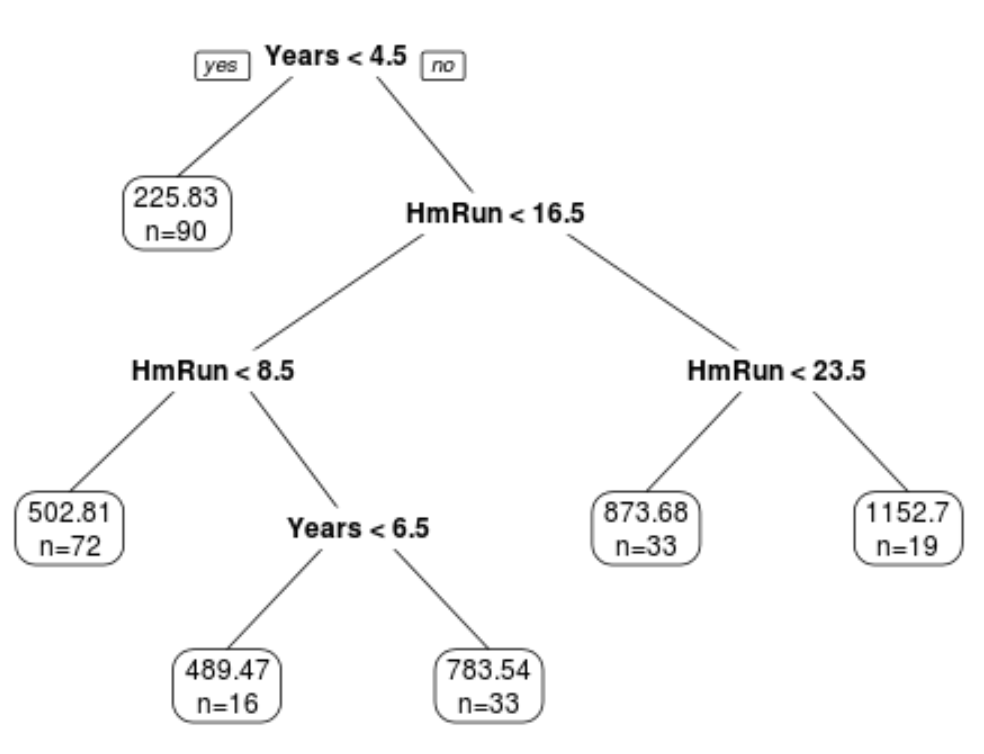
\includegraphics[width=\linewidth]{Rtree3.png}
			\caption{Regression tree}
		\end{minipage}
\end{figure}
\end{center}
\end{frame}




\begin{frame}{Forêt Aléatoire (Random Forest)}
	\begin{itemize}
	%	\item Méthode d'apprentissage automatique utilisée pour la classification et la régression
		\item Basée sur l'ensemble de plusieurs arbres de décision
		\item Chaque arbre est construit sur un sous-ensemble aléatoire des données d'entraînement et des caractéristiques
		\item Les prédictions finales sont obtenues en agrégeant les prédictions de chaque arbre (majorité pour la classification, moyenne pour la régression)
	\end{itemize}
	
	\begin{center}
		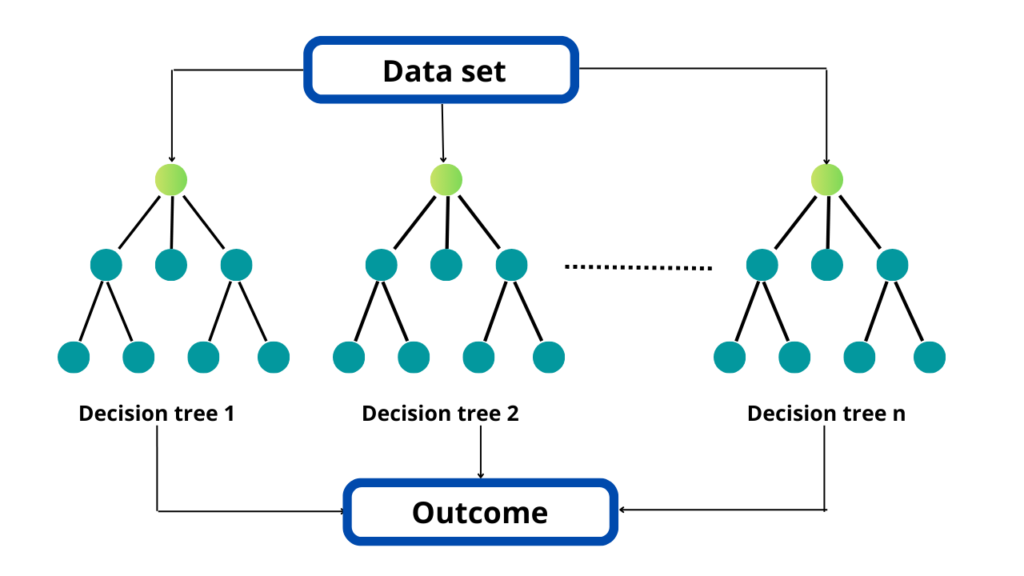
\includegraphics[width=0.6\textwidth]{destree.png}
	\end{center}
\end{frame}



\begin{frame}{Machines à Vecteurs de Support (SVM)}
	\begin{itemize}
		\item Modèle d'apprentissage automatique supervisé
		\item Utilisé pour la classification et la régression
		\item Trouve un hyperplan optimal qui sépare les données de différentes classes ou estime une fonction pour la régression
		\item Maximise la marge entre les données et l'hyperplan pour une meilleure généralisation
	\end{itemize}
	
	%\begin{center}
	%	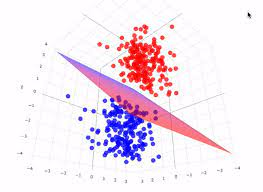
\includegraphics[width=0.6\textwidth]{csvm.jpeg}
	%\end{center}
	\begin{figure}
		\begin{minipage}[t]{0.45\linewidth}
			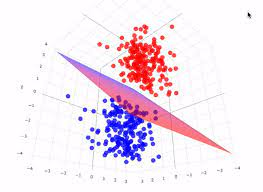
\includegraphics[width=\linewidth]{csvm.jpeg}
			\caption{Support Vector Classifier}
		\end{minipage}
		\hfill
		\begin{minipage}[t]{0.45\linewidth}
			\centering
			\includegraphics[width=\linewidth]{SVR_2.png}
			\caption{Support Vector Regressor}
		\end{minipage}
	\end{figure}
\end{frame}


\begin{frame}{Boosting}
	\begin{itemize}
		\item Technique de ML utilisée pour améliorer la performance des modèles
		\item Combinaison \color{blue} séquentielle \color{black}
		de modèles faibles pour former un fort
		\item Chaque modèle faible est entraîné à se concentrer sur les échantillons mal classés par les modèles précédents
		\item Les prédictions finales sont obtenues en agrégeant les prédictions de chaque modèle faible (pondération selon leur performance)
	\end{itemize}
	
	\begin{center}
		\includegraphics[width=0.6\textwidth]{boosting.png}
	\end{center}
\end{frame}



\begin{frame}{Boosting vs Bagging}
	\begin{columns}
		\begin{column}{0.5\textwidth}
			\textbf{Boosting}
			\begin{itemize}
				\item Combinaison séquentielle de modèles faibles
				\item Chaque modèle se concentre sur les échantillons mal classés par les modèles précédents
				\item Biais réduit, forte capacité de généralisation
				\item Sensible aux données d'entraînement bruitées ou aberrantes
			\end{itemize}
		\end{column}
		\begin{column}{0.5\textwidth}
			\textbf{Bagging}
			\begin{itemize}
				\item Combinaison parallèle de modèles indépendants
				\item Chaque modèle est entraîné sur un sous-ensemble aléatoire des données d'entraînement
				\item Réduction de la variance, faible risque de surajustement
				\item Moins sensible aux données bruitées ou aberrantes
			\end{itemize}
		\end{column}
	\end{columns}
\end{frame}


\begin{frame}{Évaluation des modèles}
	\begin{itemize}
		\item L'évaluation des modèles est essentielle pour mesurer leur performance et prendre des décisions informées.
		\item Métriques de performance couramment utilisées :
		\begin{itemize}
			\item Précision : mesure la proportion de prédictions positives correctes.
			\item Rappel : mesure la proportion de vrais positifs identifiés.
			\item F-mesure : combine la précision et le rappel en une seule métrique.
			\item Exactitude : mesure la proportion de prédictions correctes dans l'ensemble des données.
			\item Courbe ROC : représente la sensibilité (rappel) en fonction de la spécificité.
		\end{itemize}
		\item Techniques d'évaluation :
		\begin{itemize}
			\item Validation croisée : divise les données en ensembles d'entraînement et de test pour évaluer la performance.
			\item Holdout : divise les données en un ensemble d'entraînement et un ensemble de test.
			\item Bootstrap : utilise des échantillons bootstrap pour estimer la performance du modèle.
		\end{itemize}
	\end{itemize}
\end{frame}

\begin{comment}
	\begin{frame}
	\frametitle{Mesure du succès et ajustement des hyperparamètres}
	\begin{itemize}
		\item Choix des métriques appropriées pour mesurer le succès du modèle en fonction du problème
		\item Optimisation des hyperparamètres pour améliorer la performance du modèle
		\item Utilisation de méthodes comme la recherche en grille et l'optimisation bayésienne
	\end{itemize}
\end{frame}
\end{comment}




\begin{frame}{Conclusion}
	\begin{itemize}
		\item Le Machine Learning est une approche d'intelligence artificielle qui permet aux ordinateurs d'apprendre à partir des données sans être explicitement programmés.
		\item Le processus de Machine Learning comprend :
		\begin{enumerate}
			\item Collecte des données d'entraînement.
			\item Sélection du modèle approprié.
			\item Entraînement du modèle sur les données d'entraînement.
			\item Évaluation de la performance du modèle sur des données de test.
			\item Utilisation du modèle entraîné pour faire des prédictions sur de nouvelles données.
		\end{enumerate}
		\item Les algorithmes d'apprentissage automatique peuvent être supervisés ou non supervisés.
		\item L'objectif du Machine Learning est de généraliser à partir des données d'entraînement afin de faire des prédictions précises sur de nouvelles données non vues auparavant.
	\end{itemize}
\end{frame}



\section{Artificial Intelligence and Machine Learning 2}

{
\setbeamertemplate{background}{\includegraphics[width=\paperwidth,height=\paperheight]{ia_ml.jpg}}	
\begin{frame}{Artificial Intelligence and Machine Learning 2}
	%\centering
%	\includegraphics[width=\linewidth]{ia_ml.jpg}
\end{frame}

}





\begin{frame}
	\frametitle{Plan de présentation}
	\begin{itemize}
		\item Introduction
		\begin{itemize}
			\item Contexte et objectifs
		\end{itemize}
		\item XAI et IML : Explicabilité dans l'IA et le ML
		\begin{itemize}
			\item Comprendre XAI et IML
			\item Difficultés liées à l'isolation de la contribution d'une variable
			\item Modèle de boîte noire 101
		\end{itemize}
		\item KNIME pour XAI et IML
		\begin{itemize}
			\item Présentation de KNIME
			\item Utilisation de KNIME pour l'explicabilité et l'interprétabilité
			\item Exemples d'utilisation de KNIME dans XAI et IML
		\end{itemize}
		\item Techniques de XAI : Explications globales
		\begin{itemize}
			\item Obtenir des explications globales
			\item Techniques : importance des variables, arbres de décision, règles d'association, etc.
			\item Avantages et limitations des techniques d'explication globale
		\end{itemize}
		% Ajoutez les autres sections de la même manière
	\end{itemize}
\end{frame}

	
\subsection{Introduction}	
\begin{frame}{Vue d'ensemble des concepts clés}
	\begin{itemize}
		\item Qu'est-ce que l'Explainable AI (XAI) et l'Interprétabilité en ML (IML)?
		\item Les défis de l'isolement de la contribution d'une variable
		\item Modèle de boîte noire 101 : Comprendre les modèles opaques
		\item KNIME pour XAI et IML : Une introduction à l'outil
		\item Techniques d'Explainable AI (XAI) : explications globales, explications locales
		\item Techniques d'Interprétabilité en Machine Learning (IML) : visualisation, importance des variables, etc.
		\item Conception expérimentale et contrôles statistiques : l'importance de la planification et des comparaisons de modèles
		\item Conditionnel Probabilité et théorème de Bayes : Mise à jour des probabilités
		\item Prédiction et preuve avec les statistiques bayésiennes : Introduction aux statistiques bayésiennes
		\item Modélisation causale : Modélisation d'équations structurelles (SEM), réseaux bayésiens
		\item Importance d'une valeur p pour le test d'hypothèse : Définition, différence entre corrélation et causalité, démonstration de la causalité
		\item Détection de la multicolinéarité et stratégies associées
		\item Induction, déduction, falsification et contrefactuel : Importance dans l'évaluation du modèle
		\item Utilité décroissante des valeurs p avec un nombre croissant de paramètres de modèle : Explication
		\item Évaluation des performances du modèle dans l'exploration de données : Objectifs et philosophie contradictoires des statistiques et de l'exploration de données
		\item Apprentissage par renforcement : Introduction, algorithmes et méthodes associées
	\end{itemize}
\end{frame}
	
\subsection{XAI et IML : Explicabilité dans l'IA et le ML}	
\begin{frame}{Explainable AI (XAI) et Interprétabilité en ML (IML)}
\note{\begin{itemize}
		 \item L'importance de l'IML et du XAI :
	\begin{itemize}
		\item Gagner la confiance des utilisateurs et des parties prenantes.
		\item Détecter les biais et les erreurs de modélisation.
		\item Se conformer aux réglementations et aux normes éthiques.
		\item Faciliter la résolution des problèmes lorsque les modèles produisent des résultats inattendus ou incorrects.
	\end{itemize}
	\item Techniques d'IML et de XAI :
	\begin{itemize}
		\item Visualisation des caractéristiques importantes.
		\item Interprétation des poids des modèles linéaires.
		\item Méthodes d'interprétabilité spécifiques à certains algorithmes(des tree).
		\item Utilisation de modèles explicatifs, tels que les réseaux de neurones à propagation avant avec des couches interprétables. \end{itemize} \end{itemize}}
	\begin{itemize}
		\item L'Explainable AI (XAI) et l'Interprétabilité en ML (IML) visent à rendre les modèles de ML plus compréhensibles et expliquables pour les humains.
		\item L'IML : compréhension des décisions prises par les modèles, alors que le XAI vise à expliquer le fonctionnement interne des modèles.
		\item L'importance de l'IML et du XAI :
		\begin{itemize}
			\item Gagner la confiance des utilisateurs et des parties prenantes.
			\item Détecter les biais et les erreurs de modélisation.
		\end{itemize}
		\item Techniques d'IML et de XAI :
		\begin{itemize}
			\item Visualisation des caractéristiques importantes.
			\item Interprétation des poids des modèles linéaires.
		\end{itemize}
	\end{itemize}
\end{frame}
	
\begin{frame}{Les défis de l'isolement de la contribution d'une variable}
	\begin{itemize}
		\item Les défis courants de l'isolation de la contribution d'une va en ML :
		\note{		\begin{itemize}
				\item Corrélations 
				: les variables sont souvent corrélées entre elles, ce qui rend difficile de déterminer la contribution spécifique d'une variable sans tenir compte des autres.
				\item Interactions 
				: les variables peuvent interagir de manière complexe, ce qui rend difficile d'attribuer une contribution individuelle à chaque va.
				\item Non-linéarité : les relations entre les variables et la variable cible peuvent être non linéaires, ce qui complique l'isolement des contributions individuelles.
				\item Multicollinéarité
				 : lorsque plusieurs variables sont fortement corrélées, il peut être difficile de distinguer leur contribution individuelle.
		\end{itemize}}
		\begin{itemize}
			\item Corrélations 
			%: les variables sont souvent corrélées entre elles, ce qui rend difficile de déterminer la contribution spécifique d'une variable sans tenir compte des autres.
			\item Interactions 
			%: les variables peuvent interagir de manière complexe, ce qui rend difficile d'attribuer une contribution individuelle à chaque va.
			\item Non-linéarité 
			%: les relations entre les variables et la variable cible peuvent être non linéaires, ce qui complique l'isolement des contributions individuelles.
			\item Multicollinéarité
			% : lorsque plusieurs variables sont fortement corrélées, il peut être difficile de distinguer leur contribution individuelle.
		\end{itemize}
		\item Méthodes pour aborder ces défis :
		\begin{itemize}
			\item Analyse de sensibilité : évaluer l'impact d'une variable en la modifiant de manière contrôlée tout en maintenant les autres variables constantes.
			\item Décomposition de la variance : attribuer une part de la variance expliquée à chaque variable.
			\item Méthodes d'importance de variable : estimer l'importance relative des variables en utilisant des techniques telles que les arbres de décision ou les coefficients de régression.
		\end{itemize}
	\end{itemize}
\end{frame}


\begin{frame}{Modèle de boîte noire 101 : Modèles opaques}
\begin{center}
	\begin{figure}
			\includegraphics[width=0.6\linewidth]{350px-Schéma_d'une_boîte_noire.jpg}
	\end{figure}
\end{center}
	\begin{itemize}
		\item Modèles d'IA dont les mécanismes internes sont difficiles à interpréter.
		\item Modèles très performants en termes de prédiction, mais souvent difficile à comprendre.
		\item Les modèles opaques (DNN ou SVM) peuvent avoir des millions de paramètres et des architectures complexes.
		\item L'opacité de ces modèles pose des défis en termes de transparence, d'éthique et d'acceptabilité sociale de l'IA.
		\item Malgré leur complexité, XAI et IML tentent de les comprendre.
	\end{itemize}

\end{frame}



\begin{frame}{KNIME pour XAI et IML : Une introduction à l'outil}
	\note{\begin{itemize}
					\item Vous pouvez également utiliser des modules d'IML pour visualiser et interpréter les résultats de vos modèles, tels que l'importance des variables, les poids des coefficients, etc.
			\item KNIME offre une flexibilité et une extensibilité importantes, vous permettant d'adapter facilement vos workflows aux besoins spécifiques de votre projet.
	\end{itemize}}
	\begin{itemize}
		\item KNIME est une plateforme open-source d'analyse des données et de construction de workflows.
		\item Il offre une interface intuitive et conviviale pour créer, exécuter et partager des workflows d'analyse de données.
		\item KNIME propose également une large gamme de modules et d'extensions pour XAI et l'IML.
		\item Avec KNIME, vous pouvez appliquer des techniques d'XAI pour comprendre comment les modèles prennent des décisions et les expliquer de manière compréhensible.
	\end{itemize}
\end{frame}













\begin{frame}{Techniques XAI : explications globales, explications locales}
	\note{\begin{itemize}
					\item Les explications locales se concentrent sur une prédiction spécifique et fournissent une explication détaillée de la contribution de chaque variable à cette prédiction.
			\item Les techniques d'explication locale incluent des méthodes telles que les perturbations de variable, les méthodes de désensibilisation et les arbres de décision locaux.
			\item Compréhension fine des facteurs qui ont conduit à une prédiction spécifique, ce qui peut aider à détecter les biais, les erreurs ou les cas extrêmes.
	\end{itemize}}
	\begin{itemize}
		\item Les techniques XAI sont des méthodes utilisées pour expliquer les décisions prises par les modèles d'IA.
		\item Les explications globales fournissent une vue d'ensemble du modèle et de ses principaux facteurs de décision, permettant de comprendre le comportement général du modèle.
		\item Les techniques d'explication globale incluent des méthodes telles que les diagrammes d'importance de variables, les graphiques de dépendance partielle et les cartes de chaleur.
	\end{itemize}
\end{frame}

\begin{frame}{Techniques IML : visualisation, importance des variables}
	\note{\begin{itemize}
		\item Les méthodes d'importance des variables incluent l'analyse de sensibilité, le calcul des coefficients ou des poids des variables et les techniques d'élagage.
			
		\item En combinant la visualisation des données, l'importance des variables et d'autres techniques d'IML, on peut obtenir une compréhension approfondie du modèle de ML et de ses mécanismes de décision.
	\end{itemize}}
	\begin{itemize}
		\item La visualisation permet d'explorer et de comprendre les relations entre les variables et les résultats du modèle.
		\item Les graphiques, les diagrammes et les cartes peuvent être utilisés pour représenter les données de manière intuitive et faciliter l'interprétation.
		\item L'importance des variables est une autre technique d'IML qui permet d'identifier les variables qui ont le plus d'influence sur les prédictions du modèle.
	\end{itemize}
\end{frame}




\begin{frame}{Conception expérimentale et contrôles statistiques}
	\note{\begin{itemize}
				\item Une planification et des contrôles appropriés permettent de minimiser les erreurs expérimentales, d'obtenir des résultats précis et de fournir des informations utiles pour prendre des décisions éclairées en matière de modélisation.
			\item En fin de compte, la conception expérimentale et les contrôles statistiques renforcent la validité et la crédibilité des résultats obtenus à partir des modèles d'IA.
	\end{itemize}}
	\begin{itemize}

		\item Planification : définition claire des objectifs de l'expérience, choix des features à mesurer, échantillonnage.
		\item Les comparaisons de modèles
		\item Des techniques statistiques telles que les tests d'hypothèse, l'ANOVA et les tests de comparaison multiple 
		\item Il est également important de prendre en compte les biais potentiels	
	\end{itemize}
\end{frame}




\begin{frame}{Probabilité Conditionnelle et théorème de Bayes}
	\begin{itemize}
		
		\item Elle est notée $\mathbb{P}(A | B)$ et se calcule suivant la relation $$\mathbb{P}(A | B) = \frac{\mathbb{P}(A\cap B)}{\mathbb{P}(B)}$$
		\item Le théorème de Bayes permet de mettre à jour les probabilités conditionnelles lorsque de nouvelles informations sont disponibles.
		\item La formule de Bayes est donnée par  $$\mathbb{P}(A | B) = \frac{\mathbb{P}(B | A) * \mathbb{P}(A)}{\mathbb{P}(B)} $$.
		\item Le théorème de Bayes est largement utilisé dans les domaines de la statistique, du ML et de l'IA pour la prise de décision.
		\item Il permet de mettre à jour les probabilités a priori en fonction des nouvelles observations, ce qui permet d'obtenir des estimations plus précises et fiables.

%		\item En utilisant le théorème de Bayes, on peut incorporer de nouvelles informations dans un modèle probabiliste et obtenir une estimation plus précise des probabilités conditionnelles.
	\end{itemize}
\end{frame}



\begin{frame}{Introduction aux statistiques bayésiennes}
	\begin{itemize}
%		\item Les statistiques bayésiennes utilisent la théorie des probabilités bayésiennes pour modéliser et analyser les données.
		\item Contrairement aux statistiques fréquentistes, les statistiques bayésiennes considèrent les paramètres comme des v.a avec des dp.
		\item L'analyse bayésienne commence par une distribution a priori pour les paramètres, puis met à jour cette distribution en utilisant le théorème de Bayes pour obtenir une distribution a posteriori.
		\item La distribution a posteriori est utilisée pour effectuer des prédictions et des estimations, en tenant compte de l'incertitude associée aux résultats.
		\item Les statistiques bayésiennes permettent également de comparer des modèles en utilisant des facteurs de Bayes, qui intègrent la vraisemblance des données et la complexité des modèles.
		\item Les statistiques bayésiennes offrent une approche cohérente et intuitive pour la prise de décision en intégrant les connaissances préalables et les données observées.
		\item Cependant, l'analyse bayésienne peut nécessiter des techniques d'inférence approximative, telles que les chaînes de MCMC.
	\end{itemize}
\end{frame}

\begin{frame}{Statistique Bayésienne vs. Statistique Fréquentiste}
	\note{				La principale différence entre l'approche bayésienne et l'approche fréquentiste réside dans la façon de considérer les paramètres du modèle statistique.
		
		En statistique bayésienne, les paramètres sont vus comme des variables aléatoires pour lesquelles on peut définir des distributions de probabilité a priori. L'inférence se fait alors en mettant à jour ces distributions a priori en utilisant les données observées pour obtenir des distributions a posteriori des paramètres.
		
		En statistique fréquentiste, les paramètres sont considérés comme des quantités fixes inconnues. L'inférence se fait en utilisant des estimateurs ponctuels et des intervalles de confiance, basés sur la répétition d'expériences.
		
		L'approche bayésienne permet d'incorporer des connaissances préalables sur les paramètres, tandis que l'approche fréquentiste se concentre uniquement sur les données observées.}
	\textbf{Statistique Bayésienne}
	\begin{itemize}
		\item Les paramètres sont considérés comme des variables aléatoires
		\item On utilise des distributions de probabilité a priori pour les paramètres
		\item La conclusion est une distribution de probabilité a posteriori des paramètres
		\item Permet d'incorporer des connaissances préalables sur les paramètres
	\end{itemize}
	
	\vspace{0.5cm}
	
	\textbf{Statistique Fréquentiste}
	\begin{itemize}
		\item Les paramètres sont considérés comme des quantités fixes inconnues
		\item On utilise des estimateurs ponctuels et des intervalles de confiance
		\item La conclusion est une estimation ponctuelle des paramètres
		\item Se concentre sur la répétition d'expériences pour faire des inférences
	\end{itemize}
\end{frame}

\begin{frame}{Modélisation causale : Modélisation d'équations structurelles (SEM) et réseaux bayésiens}
	\note{		Ces deux approches de modélisation causale, les SEM et les réseaux bayésiens, permettent de faire des prédictions causales, d'identifier les variables clés et de tester les hypothèses causales dans un système.
		
		Les SEM se concentrent sur la représentation des relations causales à l'aide d'équations mathématiques, tandis que les réseaux bayésiens utilisent une approche graphique probabiliste qui intègre les connaissances a priori.
		
		Bien que différentes dans leur mise en œuvre, ces deux méthodes visent toutes deux à comprendre et à modéliser les liens de cause à effet entre les variables d'un système complexe.}
	\begin{itemize}
		\item La modélisation causale vise à comprendre les relations de cause à effet entre les variables dans un système.
		\item Les équations structurelles (SEM) et les réseaux bayésiens sont deux approches couramment utilisées en modélisation causale.
	\end{itemize}
	
	\vspace{0.2cm}
	
	\textbf{Modélisation d'équations structurelles (SEM)}
	\begin{itemize}
		\item Les SEM sont des modèles qui représentent les relations causales entre les variables à l'aide d'équations mathématiques.
		\item Les SEM permettent de tester des hypothèses causales.
	\end{itemize}
	
	\vspace{0.2cm}
	
	\textbf{Réseaux bayésiens}
	\begin{itemize}
		\item Les réseaux bayésiens utilisent des graphes probabilistes pour représenter les relations causales entre les variables.
		\item Les réseaux bayésiens intègrent également des connaissances a priori et des distributions de probabilité pour quantifier l'incertitude dans la modélisation causale.
	\end{itemize}	
\end{frame}





	
	
	\begin{frame}{Statistiques et tests d'hypothèse}
		\begin{itemize}
			\item La $p-$value est utilisée pour évaluer les preuves contre l'hypothèse $H_0$.
			\item Une $p-$value faible indique une preuve solide contre $H_0$.
			\item La $p-$value seule ne fournit pas d'informations sur la taille de l'effet ou la signification pratique des résultats.
			\item L'interprétation doit tenir compte de la $p-$value et de l'importance clinique ou scientifique des résultats.
		\end{itemize}
		
		\vfill
		
		\begin{itemize}
			\item La corrélation mesure la relation statistique entre deux variables.
			\item La causalité nécessite des preuves supplémentaires, comme des expérimentations contrôlées.
			\item Les études observationnelles fournissent des indications de relation causale, mais ne prouvent pas définitivement l'existence de la causalité.
		\end{itemize}
		
%		\vfill
		
		%\begin{itemize}
		%	\item La démonstration de la causalité nécessite souvent des expériences contrôlées.
		%	\item Les groupes d'expérimentation et de contrôle permettent de comparer les résultats.
		%	\item Dans certains domaines, il peut être difficile de réaliser des expériences contrôlées.
	%	\end{itemize}
	\end{frame}
	

\begin{frame}{Détection de la multicolinéarité et stratégies associées}
	\textbf{Détection de la multicolinéarité :}
	\begin{itemize}
		\item Calcul des coefficients de corrélation.
		\item Variance inflation factor (VIF).
		\item Analyse des valeurs propres.
	\end{itemize}
	
	\vfill
	
	\textbf{Stratégies pour traiter la multicolinéarité :}
	\begin{itemize}
		\item Supprimer les variables fortement corrélées.
		\item Combinaison de variables corrélées.
		\item Utilisation de techniques de régularisation (régression ridge, régression lasso).
	\end{itemize}
	
	\vfill
	
	\textbf{Remarque :} Les approches de détection et de gestion de la multicolinéarité doivent être adaptées au contexte spécifique de l'analyse et aux objectifs de modélisation.
\end{frame}


\begin{frame}{Induction, déduction, falsification et contrefactuel : Importance dans l'évaluation du modèle}
	\begin{itemize}
		\item \textbf{Induction :} Permet de généraliser à partir des observations spécifiques et de tirer des conclusions sur des situations non observées.
		\item \textbf{Déduction :} Utilisation de règles logiques pour déduire des conséquences spécifiques à partir de propositions générales. Peut aider à tester les prédictions d'un modèle.
		\item \textbf{Falsification :} Processus de recherche d'observations ou de tests qui pourraient réfuter ou invalider un modèle. Contribue à la rigueur et à la fiabilité d'un modèle.
		\item \textbf{Contrefactuel :} Étudie les effets hypothétiques d'un changement dans les conditions ou les variables. Permet d'évaluer l'impact causal et de comparer différentes situations.
	\end{itemize}
	
	\vfill
	
	L'utilisation appropriée de ces concepts contribue à une évaluation rigoureuse et solide des modèles, en tenant compte à la fois des preuves empiriques et des raisonnements logiques.
\end{frame}


\begin{frame}{Utilité décroissante des valeurs p avec un nombre croissant de paramètres de modèle : Explication}
	\begin{itemize}
		\item Lorsque le nombre de paramètres d'un modèle statistique augmente, les valeurs p associées à ces paramètres ont tendance à diminuer.
		\item Les valeurs p mesurent la significativité statistique d'un paramètre en évaluant la probabilité d'obtenir des résultats aussi extrêmes que ceux observés, sous l'hypothèse nulle.
		\item Cependant, avec un nombre croissant de paramètres, il y a une augmentation du nombre de tests statistiques effectués, ce qui peut conduire à une augmentation des chances de trouver des associations significatives par pur hasard.
		\item Ce phénomène est connu sous le nom d'utilité décroissante des valeurs p et est causé par le problème de multiplicité des tests.
		\item Plus il y a de paramètres à tester, plus il est probable d'obtenir des associations significatives par simple hasard, même en l'absence de relations réelles entre les variables.
		\item Cela souligne l'importance de prendre en compte le contexte scientifique, la taille de l'échantillon et la pertinence des relations dans l'interprétation des valeurs p.
		\item Des méthodes correctives, telles que l'ajustement de Bonferroni ou les procédures de contrôle de la fausse découverte, peuvent être utilisées pour tenir compte du problème de multiplicité des tests.
		\item Il est essentiel de considérer ces aspects lors de l'évaluation et de l'interprétation des résultats statistiques.
	\end{itemize}
\end{frame}


\begin{frame}{Évaluation des performances du modèle dans l'EDA}
	
	\note{
		Les statistiques traditionnelles et l'exploration de données ont souvent des objectifs et des philosophies contradictoires dans l'évaluation des performances du modèle.
		
		Les statistiques se concentrent davantage sur la validité et la généralisation des résultats, tandis que l'exploration de données se concentre sur la découverte de nouvelles connaissances et l'identification de modèles intéressants, même si cela implique une certaine incertitude.
		
		Cependant, il est important de reconnaître que ces deux approches sont complémentaires et peuvent être utilisées conjointement pour une évaluation plus complète des performances du modèle dans le cadre de l'exploration de données.
	}
	
	\begin{itemize}
		\item L'évaluation des performances du modèle est une étape essentielle dans l'exploration de données, visant à évaluer la qualité et l'adéquation d'un modèle pour représenter les données.
	\end{itemize}
	
	\vspace{0.2cm}
	
	\textbf{Approche statistique traditionnelle}
	\begin{itemize}
		\item Les statistiques traditionnelles se concentrent sur la précision et la validité des modèles, en utilisant des méthodes rigoureuses basées sur des hypothèses et des tests statistiques.
		\item Les statistiques mettent l'accent sur la généralisation des résultats, la réduction de l'incertitude et la déduction causale.
	\end{itemize}
	
	\vspace{0.2cm}
	
	\textbf{Approche d'exploration de données}
	\begin{itemize}
		\item L'exploration de données se concentre sur la découverte de nouvelles connaissances, l'identification de modèles intéressants et la génération d'hypothèses.
		\item L'exploration de données privilégie l'exploration des données brutes, l'utilisation de techniques non paramétriques et l'incorporation de l'expertise humaine.
		\item L'objectif de l'exploration de données est de fournir des informations exploitables et de soutenir la prise de décision, même si cela peut impliquer une certaine incertitude et une moindre généralisation.
	\end{itemize}
	
\end{frame}



\begin{frame}
	\frametitle{Conclusion}
	\begin{itemize}
		\item Récapitulatif des concepts clés abordés dans les applications pratiques de l'IA et du Machine Learning
		\item Invitation aux questions et discussions
	\end{itemize}
\end{frame}

\section{Artificial Intelligence and Machine Learning 3}

{
	\setbeamertemplate{background}{\includegraphics[width=\paperwidth,height=\paperheight]{ia_ml.jpg}}
\begin{frame}{Artificial Intelligence and Machine Learning 3}
	%\centering
	%\includegraphics[width=\linewidth]{ia_ml.jpg}
\end{frame}

}




\begin{frame}
	\frametitle{Plan de présentation}
	\begin{itemize}
		\item Examen des défis de l'IA
		\item Application de l'IA étroite à une décision
		\item Définition de deux approches efficaces utilisées face à l'IA
		\item Examen de l'apprentissage supervisé et non supervisé
		\item Explication du harcèlement par l'IA
		\item Identification de trois concepts sur lesquels repose la justice distributive
		\item Avantages et limites de XAI
		\item Humains par rapport aux ordinateurs
		\item Exemples commerciaux de XAI
		\item Investir dans XAI
		% Ajoutez les autres sections de la même manière
	\end{itemize}
\end{frame}
\begin{frame}{Plan de présentation}
	\begin{itemize}
			
	\item Transformateurs en PNL
	\item Formation des transformateurs et leur architecture
	\item Grands modèles de langage
	\item Présentation des arbres de décision
	\item Présentation de l'algorithme C5.0
	\item Présentation des arbres de classification
	\item Présentation des arbres de régression
	\item NPL et transformateurs
	\item BERT et apprentissage par transfert
	\item Architecture de transformateur et BERT
	\item Classification de texte
\end{itemize}
\end{frame}

\subsection{Examen des défis de l'IA}
\begin{frame}{Examen des défis de l'IA}
	\begin{columns}[T]
		\begin{column}{0.5\textwidth}
			\begin{itemize}
				\item Manque de transparence des modèles d'IA
				\item Biais et résultats discriminatoires
				\item Problèmes d'éthique et de confidentialité
				\item Impact sur l'emploi
				\item Besoin de big data
				\item Sécurité des systèmes d'IA
			\end{itemize}
		\end{column}
		\begin{column}{0.5\textwidth}
			\includegraphics[width=\textwidth]{AI-ethics.jpg}
		\end{column}
	\end{columns}
\end{frame}

\begin{frame}{Application de l'IA étroite à une décision}
	\begin{itemize}
		\item L'IA étroite ou IA faible, se réfère à des systèmes d'IA conçus pour effectuer des tâches spécifiques avec une grande précision.
		\item Ces systèmes d'IA sont utilisées en reconnaissance d'image, traduction automatique, détection de fraude, etc.
		\item L'IA étroite est utilisée dans les systèmes de recommandation personnalisée ou les chatbots de service client.
		\item Les systèmes d'IA étroite utilisent des algorithmes sophistiqués et des techniques de ML.
		\item Limites: incapacité à reproduire pleinement les capacités cognitives humaines (compréhension du contexte, de flexibilité et de raisonnement abstrait).
		%\item Compréhension des domaines dans lesquels l'IA étroite peut être appliquée de manière efficace et les limites de son utilisation afin d'éviter des erreurs ou des résultats inappropriés.
	\end{itemize}
\end{frame}

\begin{frame}{Définition de deux approches efficaces utilisées face à l'IA}
	\begin{columns}[T]
		\begin{column}{0.5\textwidth}
			\textbf{Apprentissage supervisé}
			\begin{itemize}
				\item Utilise des données étiquetées
				\item Prédit des résultats pour de nouvelles données
				\item Exemples : classification, prédiction
			\end{itemize}
		\end{column}
		\begin{column}{0.5\textwidth}
			\textbf{Apprentissage non supervisé}
			\begin{itemize}
				\item Utilise des données non étiquetées
				\item Découvre des structures, des modèles ou des relations
				\item Exemples : regroupement, réduction de dimensionnalité
			\end{itemize}
		\end{column}
	\end{columns}
	\vspace{0.5cm}
	\centering
	\includegraphics[width=0.8\textwidth]{approachesdata.png}
\end{frame}





\begin{frame}{Explication du harcèlement par l'IA}
	\begin{columns}[T]
		\begin{column}{0.6\textwidth}
			\begin{itemize}
				\item Génération de contenu haineux
				\item Ciblage et traque en ligne
				\item Biais et discrimination
			\end{itemize}
		\end{column}
		\begin{column}{0.4\textwidth}
			\includegraphics[width=\textwidth]{harcellement.png}
		\end{column}
	\end{columns}
	
	\vspace{0.5cm}
	
	\begin{itemize}
		\item Les modèles d'IA peuvent être exploités pour générer automatiquement du contenu haineux et offensant.
		\item Les algorithmes d'IA peuvent être utilisés pour cibler et harceler des individus en ligne.
		\item Les biais et préjugés présents dans les données d'entraînement peuvent conduire à une discrimination automatique.
	\end{itemize}
\end{frame}


\begin{frame}{Concepts clés de la justice distributive}
	 \note{
		La justice distributive est un concept clé en philosophie politique et en éthique, qui traite de la répartition équitable des ressources, des avantages et des charges au sein d'une société. Trois principes fondamentaux sont généralement considérés comme les piliers de la justice distributive : l'égalité, les besoins et le mérite. Ces principes peuvent parfois entrer en conflit et nécessitent un équilibre dans leur application.
	}
	\textbf{Égalité}
	\begin{itemize}
		\item Principe fondamental de la justice distributive
		\item Répartition équitable des ressources et des avantages
		\item Élimination de la discrimination basée sur des features personnelles
	\end{itemize}
	
	\vspace{0.3cm}
	
	\textbf{Besoins}
	\begin{itemize}
		\item Prise en compte des besoins réels des individus
		\item Attribution des ressources en fonction des besoins urgents ou essentiels
		\item Exemple : priorité d'accès aux soins pour les personnes malades
	\end{itemize}
	
	\vspace{0.3cm}
	
	\textbf{Mérite}
	\begin{itemize}
		\item Distribution des ressources en fonction du mérite ou de la contribution
		\item Récompense des gens pour leur travail, compétences ou contribution
		\item Exemple : rémunération plus élevée pour les compétences spécialisées ou les emplois valorisés
	\end{itemize}
\end{frame}

\subsection{XAI (IA explicative)}
\begin{frame}{XAI (IA explicative)}
 Rendre les décisions des IA explicables pour les utilisateurs humains.
	\begin{itemize}
		\item Avantages de XAI :
		\begin{itemize}
			\item Compréhension des décisions des modèles d'IA.
			\item Détection des biais et des erreurs dans les prédictions.
			\item Renforcement de la confiance des utilisateurs dans les systèmes d'IA.
		\end{itemize}
		\item Limites de XAI :
		\begin{itemize}
			\item Certaines IA sont intrinsèquement opaques et difficiles à expliquer.
			\item XAI peut ne pas refléter pleinement la complexité du modèle.
			\item Explicabilité et performance des modèles délicat à atteindre.
		\end{itemize}
		\item Exemples commerciaux de XAI :
		\begin{itemize}
			\item Systèmes de recommandation personnalisée expliquant les suggestions.
			\item Modèles d'IA pour la détection de fraude expliquant les classifications.
			\item Chatbots explicatifs expliquant le raisonnement derrière leurs réponses.
		\end{itemize}
		\item Importance d'investir dans XAI :
		\begin{itemize}
			\item Renforcement de la transparence et de la responsabilité des IA.
			\item Réduction des risques liés aux décisions automatisées.
			\item Adoption plus large et acceptation sociale de l'IA.
		\end{itemize}
	\end{itemize}
\end{frame}


\subsection{Natural Language Processing}
\begin{frame}[t]{Transformateurs en PNL}
	\setbeamercolor{item}{fg=blue}
	\setbeamertemplate{itemize items}[circle]
	
			\textbf{Architecture du transformateur}
			\begin{itemize}
				\item Les couches d'attention capturent les relations entre les mots.
				\item Pas besoin de modèles récurrents ou de convolutions.
			\end{itemize}
			
			
			\textbf{Formation des transformateurs}
			\begin{itemize}
				\item Apprentissage supervisé avec des tâches spécifiques.
				\item Entraînement sur de grandes quantités de données annotées.
			\end{itemize}	
		
	\textbf{Applications en PNL}
	\begin{itemize}
		\item Traduction automatique
		\item Génération de texte et Compréhension du langage
	\end{itemize}
	\centering
\includegraphics[width=0.8\textwidth]{PNL.png}	

	\textbf{Avantages des transformateurs}
	\begin{itemize}
		\item Capture des dépendances à longue distance.
		\item Modélisation des relations complexes entre les mots.
		\item Performances supérieures sur de nombreuses tâches de PNL.
	\end{itemize}
\end{frame}

\begin{frame}[t]{Grands modèles de langage}
	\setbeamercolor{item}{fg=blue}
	\setbeamertemplate{itemize items}[circle]
	\begin{itemize}
		\item Les grands modèles de langage révolutionnent le PNL.
		\item Basés sur les transformateurs, des architectures de réseaux np.

		\item GPT (Generative Pre-trained Transformer) : Apprentissage non supervisé, excellente génération de texte.
		\item BERT (Bidirectional Encoder Representations from Transformers) : Apprentissage supervisé, diverses tâches de PNL.
		\item T5 (Text-to-Text Transfer Transformer) : toutes les tâches de PNL.
	\end{itemize}
	\centering
\includegraphics[width=0.6\textwidth]{Best-Large-Language-Models.jpg}
\end{frame}




\begin{frame}[t]{NLP et transformateurs}
	\setbeamertemplate{itemize items}[circle]
	
	\textbf{Traitement du langage naturel (NLP)}
	\begin{itemize}
		\item IA qui se concentre sur l'interaction ordinateurs - langage h.
		\item Traduction, génération de texte, compréhension du langage
	\end{itemize}
	
	\textbf{Transformateurs}
	\begin{itemize}
		\item Prise en compte des dépendances dans les séquences.
		\item Élimine le besoin de modèles récurrents ou de convolutions
	\end{itemize}

	\centering
	\includegraphics[width=0.4\textwidth]{blog-NLP-pic1.png}
\end{frame}


\begin{frame}[t]{Présentation de l'algorithme C5.0}
	\begin{itemize}
		\item Collecte des données étiquetées pour la classification.
		\item Construction d'un arbre de décision en sélectionnant la meilleure variable d'entrée à chaque nœud.
		\item Prédiction des classes pour les exemples non étiquetés.
		\item Élagage de l'arbre pour améliorer la généralisation.
	\end{itemize}
	
	\centering
	\includegraphics[width=0.5\textwidth]{C50-decision-tree.png}
	
	\begin{itemize}
		\item Avantages de C5.0 : adaptabilité aux variables discrètes ou continues, gestion des ensembles de données volumineux, interprétabilité de l'arbre de décision.
	\end{itemize}
\end{frame}

















\section{AI and ML 4 : Cas Pratique}
{
	\setbeamertemplate{background}{\includegraphics[width=\paperwidth,height=\paperheight]{ia_ml.jpg}}
	\begin{frame}{Artificial Intelligence and Machine Learning 4}
		%\centering
		%\includegraphics[width=\linewidth]{ia_ml.jpg}
	\end{frame}
	
}

\begin{frame}
	\frametitle{Plan de présentation}
	\begin{itemize}
		\item Power BI

			\begin{itemize}
			\item Analyse d'une variable unique et relations entre les variables
		%	\item Mesure des relations entre les variables
			\item Utilisation de visuels d'IA pour poser des questions de simulation
		%	\item Analyse de données de séries chronologiques
			\item Création et partage d'analyses
		\end{itemize}

		\item Chatbots avec Azure
			\begin{itemize}
			\item Introduction aux chatbots
			\item Terminologie et architecture des chatbots
			\item Conception d'un chatbot et amélioration des actions
		\end{itemize}
		\item Chatbots via Google Dialogflow
			\begin{itemize}
			\item Blocs de construction Dialogflow
			\item Configuration d'un compte Dialogflow
			\item Création des intentions
		%	\item Importation et exportation d'un agent
		%	\item Création des entités et des paramètres
		%	\item Ajout des intentions de suivi
		%	\item Contexte d'entrée et de sortie
		%	\item Création d'un épanouissement
		%	\item Intégration d'un chatbot à votre site Web
		\end{itemize}
		\item Machine Learning avec Scikit-Learn
			\begin{itemize}
			\item Pourquoi utiliser Scikit-learn
			\item Apprentissage supervisé ou non supervisé
			\item Clustering K-means
			\item Analyse en composantes principales (ACP)
		\end{itemize}
		% Ajoutez les autres sections de la même manière
	\end{itemize}
\end{frame}

\subsection{Power BI}
\begin{frame}
	\frametitle{Power BI : Business Intelligence pour tous}
	
	\begin{columns}[T] % Deux colonnes pour organiser le texte et le graphique
		\begin{column}{0.5\textwidth}
			\begin{itemize}
				\item Power BI, plateforme de BI développée par Microsoft.
				\item Importer, visualiser et analyser les data  interactivement.
				\item Data Analyst, Responsable d'entreprise ou utilisateurs.
				\item Transformer et modéliser les data.
				\item Créer des tableaux de bord interactifs et attrayants pour partager vos analyses..
			\end{itemize}
		\end{column}
		\begin{column}{0.5\textwidth}
			% Insérez ici votre code pour le graphique, par exemple avec TikZ ou en incluant une image
			\begin{center}
				\includegraphics[width=\textwidth]{power-bi-data.jpg}
			\end{center}
		\end{column}
	\end{columns}
	
\end{frame}


\begin{frame}
	\frametitle{Analyse d'une variable unique}
	
	\begin{itemize}
		\item Une fois les données importées, vous pouvez effectuer des analyses sur une variable unique.
		\item Représenter graphiquement la distribution de la variable.
		\item Créer des histogrammes, diagrammes en boîte, des diagrammes à barres, etc.
		\item Ces visualisations vous aident à comprendre les tendances, les valeurs aberrantes et les diverses caractéristiques de la variable.
	\end{itemize}
	
\end{frame}


\begin{frame}
	\frametitle{Mesure des relations entre les variables}
	
	\begin{itemize}
		\item Les diagrammes de dispersion (scatter plots).
		\item Analyse statistique (coefficients de corrélation) pour quantifier la force et la direction des relations entre les variables.
		\item Comprendre les dépendances entre les différentes variables et à identifier les facteurs qui influencent vos données.
		\item En explorant les relations entre les variables, vous pouvez prendre des décisions éclairées et développer des modèles prédictifs plus précis.
	\end{itemize}
	
\end{frame}




\begin{frame}
	\frametitle{Utilisation de visuels d'IA pour poser des questions de simulation}
	
	\begin{itemize}
		\item Power BI intègre des fonctionnalités d'IA pour vous permettre de poser des questions de simulation à vos données.
		\item Vous pouvez utiliser des visuels d'IA, tels que les cartes de tendance temporelle prédictive, pour obtenir des prévisions et des simulations basées sur vos données historiques.
		\item Ces visuels vous aident à explorer différents scénarios et à évaluer l'impact de différentes variables sur vos résultats.
		\item Par exemple, vous pouvez simuler l'effet d'une augmentation des prix sur les ventes ou visualiser l'évolution attendue d'une métrique au fil du temps.
		\item En utilisant ces visuels d'IA, vous pouvez prendre des décisions plus éclairées et anticiper les résultats potentiels de vos actions.
	\end{itemize}
	
\end{frame}


\begin{frame}[t]{Modèle de série chronologique}
	\setbeamertemplate{itemize items}[circle]
	
	\textbf{Qu'est-ce qu'une série chronologique ?}
	\begin{itemize}
		\item Une série chronologique est une collection de données organisées selon un ordre temporel.
		\item Chaque observation est associée à une date ou un instant précis.
		\item Les séries chronologiques peuvent être univariées  ou multivariées.
	\end{itemize}
	
	\vspace{0.3cm}
	\textbf{Modélisation de séries chronologiques}
	\begin{itemize}
		\item L'objectif de la modélisation de séries chronologiques est de comprendre les motifs, les tendances et les comportements dans les données temporelles.
		\item Les modèles de séries chronologiques utilisent des équations mathématiques pour décrire et prévoir les données.
		\item Les techniques de modélisation: ARIMA, modèles de lissage exponentiel, les réseaux de neurones récurrents (RNN) et les modèles basés sur les états cachés.
	\end{itemize}
\end{frame}

\begin{frame}{Modèles mathématiques de série chronologique}
	
	\note{
		Les modèles mathématiques de série chronologique sont utilisés pour analyser et prédire le comportement des données temporelles. Ils se basent sur des équations qui décrivent la structure et la dynamique des données dans le temps. Cette formalisation mathématique permet d'étudier les différents composants d'une série chronologique et d'appliquer des méthodes statistiques avancées pour la modélisation et la prévision.
	}
	

	
	\textbf{Composants d'une série chronologique}
	\begin{itemize}
		\item Tendance : évolution à long terme de la série
		\item Saisonnalité : variations périodiques (jour, mois, trimestre, etc.)
		\item Cycle : fluctuations à moyen terme
		\item Résidu : composante aléatoire non expliquée
	\end{itemize}

	\begin{equation*}
\text{	\textbf{Modèle général}}:		Y_t = f(t) + s(t) + c(t) + \epsilon_t   \; \text{,	où :}
	\end{equation*}
	\begin{itemize}
		\item $Y_t$ : valeur de la série au temps $t$
		\item $f(t)$ : composante de tendance
		\item $s(t)$ : composante saisonnière
		\item $c(t)$ : composante cyclique
	\end{itemize}
	\textbf{Exemples de modèles spécifiques}
	\begin{itemize}
		\item Modèle autorégressif (AR)
		\item Modèle à moyenne mobile (MA)
		\item Modèle ARIMA (autorégression intégrée à moyenne mobile)
	\end{itemize}
	
\end{frame}

\begin{frame}[t]{Mise en œuvre de l'analyse de séries chronologiques}
	\setbeamertemplate{itemize items}[circle]
	
	\textbf{Visualisation des séries chronologiques}
	\begin{itemize}
		\item Importez vos données de séries chronologiques dans Power BI.
		\item Utilisez des visualisations appropriées pour afficher les tendances, les motifs saisonniers et les variations.
	\end{itemize}
	
	\vspace{0.3cm}
	\textbf{Prévision des séries chronologiques}
	\begin{itemize}
		\item Utilisez les équations mathématiques des modèles de séries chronologiques pour générer des prévisions.
		\item Les modèles ARIMA, par exemple, sont basés sur les équations AR (AutoRegressive), MA (Moving Average) et I (Integrated) pour capturer les motifs, les tendances et les erreurs.
	\end{itemize}
	
	\vspace{0.3cm}
	\textbf{Analyse des séries chronologiques}
	\begin{itemize}
		\item Utilisez les fonctions DAX pour calculs et analyses des séries chrono.
		\item Les moyennes mobiles, les décompositions saisonnières et les tests stat
	\end{itemize}
\end{frame}

\subsection{Chatbots avec Azure}





\subsection{Chatbots avec Dialogflow}



\section{Python for Machine Learning 1: Initiation}
{
	\setbeamertemplate{background}{\includegraphics[width=\paperwidth,height=\paperheight]{py.jpg}}
	\begin{frame}{Python 1 : Initiation}
		%\centering
		%\includegraphics[width=\linewidth]{py.jpg}
	\end{frame}
}


\begin{frame}
	\frametitle{Plan de présentation}
	\begin{itemize}
		\item Apprentissage automatique avec Python
		%\item Apprentissage automatique
		\item Découverte de modèles avec des règles d'association
		\item Réseaux de neurones en Python
		\item Choix d'un réseau de neurones
		\item Les éléments constitutifs des réseaux de neurones
		\item Construction de votre réseau
		\item Formation de votre réseau
		\item Création d'un affichage de segments classificateur
		% Ajoutez les autres sections de la même manière
	\end{itemize}
\end{frame}


\subsection{Machine Learning with Python}
\begin{frame}{Python}
	\begin{figure}
		\includegraphics[width=\textwidth]{PythonIDE.jpg}
	\end{figure}
\end{frame}


%\subsection{From Understanding to Approach}
\begin{frame}{From Understanding to Approach}
		Supposons que nous souhaitons automatiser le processus de détermination de la cuisine d'un plat ou d'une recette donnée. 
	\begin{figure}
		\includegraphics[width=\textwidth]{From Understanding to Approach.png}
	\end{figure}
\end{frame}


	\begin{frame}{Cuisines}
	
	\begin{figure}[h]
		\centering
		\begin{minipage}{0.4\textwidth}
			\centering
			\includegraphics[width=0.5\linewidth]{photo1.jpg}
			\caption{Atayef and Ma'mul - Balha's Pastry}
		\end{minipage}\hfill
		\begin{minipage}{0.45\textwidth}
			\centering
			\includegraphics[width=0.7\linewidth]{photo2.jpg}
			\caption{Avgolemono Soup and Grilled Chicken}
		\end{minipage}
	
		\begin{minipage}{0.45\textwidth}
			\centering
			\includegraphics[width=0.5\linewidth]{photo3.jpg}
			\caption{Bacon and cheese}
		\end{minipage}\hfill
		\begin{minipage}{0.45\textwidth}
			\centering
			\includegraphics[width=0.5\linewidth]{photo4.jpg}
			\caption{Baguette french toast}
		\end{minipage}
	\end{figure}
	
\end{frame}	


\begin{frame}{Business understanding : Automating Cuisine Identification} 
		\begin{itemize}
	\item Definition of the problem and its importance.
	\item Identifying the key stakeholders and their objectives.
	\item Gathering domain knowledge and understanding business requirements.
\end{itemize}
\begin{enumerate}
	\item[2-] En regardant le diagramme, nous repérons  deux caractéristiques remarquables de la méthodologie de la DS. Lesquelles?
	\item[3-] Pouvons-nous prédire la cuisine d'un plat donné en utilisant uniquement le nom du plat ?
	\item[4-] Et en utilisant uniquement l'apparence ? Est-il possible de prédire la cuisine d'un plat donné ?
\end{enumerate}
Automatiser le processus de détermination de la cuisine d'un plat donné n'est donc pas un problème simple.

\begin{itemize}
	\item[5-] Que dire de la détermination de la cuisine d'un plat en fonction de ses ingrédients ?
\end{itemize}
\end{frame}



\begin{frame}
	\frametitle{Analytic Approach: Automating Cuisine Identification}
	
	\begin{itemize}
			\item Questions to consider:
			\begin{enumerate}
				\item What are the available data sources?
				\item Which features can be extracted from the data?
				\item Are there existing models or algorithms that can be leveraged?
				\item How can the accuracy of the predictions be evaluated?
			\end{enumerate}
			\item Informative Decision Tree:
			\vspace{0.5cm}
			\begin{center}
				% Insert your decision tree diagram here
				\includegraphics[width=0.6\textwidth]{informativetree.png}
			\end{center}
		\end{itemize}
	 Conclusion: The goal of this stage is expressing the problem in the context of statistical and ml techniques
\end{frame}






\begin{frame}{Requirements}
	\begin{figure}
		\includegraphics[width=\textwidth]{requirements.png}
	\end{figure}
\end{frame}

\begin{frame}{Data collection for Machine Learning}
	\begin{figure}
		\includegraphics[width=\textwidth]{data collection.png}
	\end{figure}
\end{frame}


\begin{frame}{Data understanding}
	\begin{figure}
		\includegraphics[width=\textwidth]{data understanding .png}
	\end{figure}
	The data we need to answer the question, \textbf{\textit{can we automate the process of determining the cuisine of a given recipe}}?, is readily available. Researcher \textbf{Yong-Yeol Ahn} scraped tens of thousands of food recipes (cuisines and ingredients).
\end{frame}






\begin{frame}[fragile]
	\frametitle{Data understanding}	
	\framesubtitle{Import libraries and download Data}
	\begin{lstlisting}
import pandas as pd # import library to read data
pd.set_option('display.max_columns', None)
import numpy as np # import numpy library
import re # import library for regular expression
recipes = pd.read_csv("https://cf-courses-data.s3.us.cloud-object-storage.appdomain.cloud/IBMDeveloperSkillsNetwork-DS0103EN-SkillsNetwork/labs/Module%202/recipes.csv") # 30 s
	\end{lstlisting}
\begin{lstlisting}
recipes.head()	
recipes.shape
ingredients = list(recipes.columns.values)
\end{lstlisting}	
\end{frame}

\begin{frame}{Data understanding}
	\framesubtitle{Description du jeu de données}
	Notre jeu de données est composé de 57 691 recettes. Chaque ligne représente une recette, et pour chaque recette, la cuisine correspondante est documentée, ainsi que la présence de 384 ingrédients dans la recette. Nous savons qu'une recette de sushi de base comprend les ingrédients suivants :
\begin{itemize}
	\item Riz
	\item Sauce soja
	\item Wasabi
	\item Du poisson/légumes au choix
\end{itemize}
\end{frame}


\begin{frame}[fragile]
	\frametitle{Data Preparation}
	\framesubtitle{Frequency Table}	
This stage involves exploring the data further and making sure that it is in the right format for the machine learning algorithm that we selected in the analytic approach stage.
	\begin{lstlisting}
		recipes["country"].value_counts()
	\end{lstlisting}
By looking at the table, we can make the following observations:

\begin{itemize}
	\item  Cuisine column is labeled as Country, which is inaccurate.
\item   Cuisine names are not consistent as not all of them start with an uppercase first letter.
\item   Some cuisines are duplicated as variation of the country name, such as Vietnam and Vietnamese.
\item   Some cuisines have very few recipes.

\end{itemize}	
\end{frame}

\begin{frame}[fragile]
	\frametitle{Data Preparation}
	\framesubtitle{Let's fix these problems}
	\begin{enumerate}
		\item Fix the name of the column showing the cuisine
		\begin{lstlisting}
column_names = recipes.columns.values
column_names[0] = "cuisine"
recipes.columns = column_names
		\end{lstlisting}
		\item Make all the cuisine names lowercase
		\begin{lstlisting}
recipes["cuisine"] = recipes["cuisine"].str.lower()
		\end{lstlisting}
	\item Make the cuisine names consistent.
	\end{enumerate}
\begin{lstlisting}
recipes.loc[recipes["cuisine"] == "austria", "cuisine"] = "austrian"
recipes.loc[recipes["cuisine"] == "belgium", "cuisine"] = "belgian"
recipes.loc[recipes["cuisine"] == "china", "cuisine"] = "chinese"
\end{lstlisting}
\end{frame}



\begin{frame}[fragile]
	\frametitle{Data Preparation}
	\framesubtitle{Let's fix these problems}
\begin{itemize}
	\item Convert all Yes's to $1$'s and the No's to $0$'s
	\begin{lstlisting}
recipes = recipes.replace(to_replace="Yes", value=1)
recipes = recipes.replace(to_replace="No", value=0)
	\end{lstlisting}
\item Recipes that contain rice and soy and wasabi and seaweed
\begin{lstlisting}
check_recipes = recipes.loc[(recipes["rice"] == 1) & (recipes["soy_sauce"] == 1) & (recipes["wasabi"] == 1) & (recipes["seaweed"] == 1)
	]
check_recipes
\end{lstlisting}
\end{itemize}
Based on the results of the above code, can we classify all recipes that contain rice and soy and wasabi and seaweed as Japanese recipes? Why?
\end{frame}



\begin{frame}[fragile]
	\frametitle{Data Preparation}
	\framesubtitle{Learn the data better}
	\begin{enumerate}
\item Let's count the ingredients across all recipes.
	\begin{lstlisting}
ing = recipes.iloc[:, 1:].sum(axis=0) #sum column
	
# define each column as a pandas series
ingredient = pd.Series(ing.index.values, index = np.arange(len(ing)))
count = pd.Series(list(ing), index = np.arange(len(ing)))

# create the dataframe
ing_df = pd.DataFrame(dict(ingredient = ingredient, count = count))
ing_df = ing_df[["ingredient", "count"]]
print(ing_df.to_string())
\end{lstlisting}
	\end{enumerate}

\end{frame}


\begin{frame}[fragile]
	\frametitle{Data Preparation}
	\framesubtitle{Learn the data better}
	\begin{enumerate}
		\item What are the 3 most popular ingredients?
		\begin{lstlisting}
ing_df.sort_values(["count"], ascending=False, inplace=True)
ing_df.reset_index(inplace=True, drop=True)

print(ing_df)
		\end{lstlisting}
	\item However, note that there is a problem with the above table. There are ~40,000 American recipes in our dataset, which means that the data is biased towards American ingredients. \textbf{Let's create a profile for each cuisine.}
	\begin{lstlisting}
cuisines = recipes.groupby("cuisine").mean()
cuisines.head()
	\end{lstlisting}
	\end{enumerate}
	
\end{frame}



\begin{frame}[fragile]
	\frametitle{Data Preparation}
	\framesubtitle{Learn the data better}
	\begin{enumerate}
		\item What are the 3 most popular ingredients?
		\begin{lstlisting}
ing_df.sort_values(["count"], ascending=False, inplace=True)
ing_df.reset_index(inplace=True, drop=True)
			
print(ing_df)
		\end{lstlisting}
	\end{enumerate}
	
\end{frame}


\begin{frame}[fragile]
	\frametitle{Data Preparation}
	\framesubtitle{Learn the data better: Top four ingredients in each cuisine}
		\begin{lstlisting}
num_ingredients = 4 # number of top ingredients
# function that prints the top ingredients for each c
def print_top_ingredients(row):
	print(row.name.upper())
	row_sorted = row.sort_values(ascending=False)*100
	top_ingredients = list(row_sorted.index.values)[0:num_ingredients]
	row_sorted = list(row_sorted)[0:num_ingredients]

	for ind, ingredient in enumerate(top_ingredients):
		print("%s (%d%%)" % (ingredient, row_sorted[ind]), end=' ')
create_cuisines_profiles = cuisines.apply(print_top_ingredients, axis=1)
		\end{lstlisting}	
\end{frame}




\begin{frame}{Data Modelling}
	\begin{figure}
		\includegraphics[width=\textwidth]{Modelling.png}
	\end{figure}
\end{frame}


\begin{frame}[fragile]
	\frametitle{Download and install dependencies to build decision trees}
\begin{lstlisting}
	# import decision trees scikit-learn libraries
	%matplotlib inline
	from sklearn import tree
	from sklearn.metrics import accuracy_score, confusion_matrix
	
	import matplotlib.pyplot as plt
	
	# If running locally, you can try using the graphviz library but we'll use sklearn's plot_tree method
	# !conda install python-graphviz --yes
	# from sklearn.tree import export_graphviz
	
	import itertools
\end{lstlisting}
\end{frame}

\frame{
	\frametitle{Creating Decision Trees for Asian and Indian Cuisines}
	
	\begin{itemize}
		\item In this project, we are focusing on creating a decision tree for recipes from Asian (Korean, Japanese, Chinese, Thai) and Indian cuisines.
		\item The reason for this approach is that the decision tree algorithm may not perform well when the dataset is biased towards one cuisine, such as American cuisines.
		\item Instead of excluding the American cuisines from our analysis, we have chosen to build decision trees for different subsets of the data.
		\item By focusing on specific subsets, we can better capture the unique characteristics and features of each cuisine, leading to more accurate and meaningful decision trees.
	\end{itemize}
}


\begin{frame}[fragile]
	\frametitle{Building Decision Trees for Asian and Indian Cuisines}
	\begin{lstlisting}
# select subset of cuisines
asian_indian_recipes = recipes[recipes.cuisine.isin(["korean", 		
  "japanese",
  "chinese",
  "thai",
  "indian"])]
  
cuisines = asian_indian_recipes["cuisine"]
ingredients = asian_indian_recipes.iloc[:,1:]
		
bamboo_tree = tree.DecisionTreeClassifier(max_depth=3)
bamboo_tree.fit(ingredients, cuisines)
		
print("Decision tree model saved to bamboo_tree!")
	\end{lstlisting}
\end{frame}




\begin{frame}[fragile]
	\frametitle{Visualizing Decision Tree for Asian and Indian Cuisines}

%To visualize the decision tree for our analysis, we use the \texttt{plot\_tree} function provided by the \texttt{tree} module in Scikit-learn.

	
\begin{lstlisting}
plt.figure(figsize=(40,20))
_ = tree.plot_tree(bamboo_tree,
feature_names = list(ingredients.columns.values),
class_names=np.unique(cuisines),filled=True, node_ids=True, impurity=False, label="all", fontsize=20, rounded = True)
plt.show()
\end{lstlisting}
	
	\begin{itemize}
		\item The decision tree provides insights into the distinguishing features of different cuisines.
		\item Based on the tree, we can make predictions about the cuisine of a recipe based on its ingredients.
		\item For example, if a recipe contains cumin and fish but no yogurt, it is most likely a Thai recipe.
		\item On the other hand, if a recipe contains cumin but no fish and no soy sauce, it is most likely an Indian recipe.
	\end{itemize}
\end{frame}


\begin{frame}{Model Evaluation}
	\begin{figure}
		\includegraphics[width=\textwidth]{Modelling.png}
	\end{figure}
\end{frame}


\begin{frame}[fragile]
	\frametitle{Evaluating the Model for Asian and Indian Cuisines}
	
	\begin{itemize}
		\item To evaluate our model for Asian and Indian cuisines, we will split our dataset into a training set and a test set.
		\item This will allow us to assess the performance of the decision tree model and compare the predicted cuisines to the actual cuisines.
		\item Let's start by creating a new dataframe called "bamboo" that contains only the data pertaining to the Asian and Indian cuisines.
	\end{itemize}
\begin{lstlisting}
bamboo = recipes[recipes.cuisine.isin(["korean", "japanese", "chinese", "thai", "indian"])]
bamboo["cuisine"].value_counts()
\end{lstlisting}

\begin{itemize}
\item By creating this new dataframe, we can focus our analysis on the specific cuisines of interest.
\item Next, we will proceed to split the dataset into a training set and a test set for model evaluation.
\end{itemize}

\end{frame}


\begin{frame}[fragile]
	\frametitle{Evaluating the Model for Asian and Indian Cuisines}
	\framesubtitle{Split data into traning and test set}
	\begin{itemize}
\item  Let's remove 30 recipes from each cuisine to use as the test set
	\begin{lstlisting}
sample_n = 30 # set sample size
random.seed(1234) # set random seed
bamboo_test = bamboo.groupby("cuisine", group_keys=False).apply(lambda x: x.sample(sample_n))
# ingredients
bamboo_test_ingredients = bamboo_test.iloc[:,1:]
# corresponding cuisines or labels 
bamboo_test_cuisines = bamboo_test["cuisine"] 
	\end{lstlisting}
\item Let's create the training set by removing the test set
\begin{lstlisting}
bamboo_test_index = bamboo.index.isin(bamboo_test.index)
bamboo_train = bamboo[~bamboo_test_index]
bamboo_train_ingredients = bamboo_train.iloc[:,1:] 
bamboo_train_cuisines = bamboo_train["cuisine"]
\end{lstlisting}
	\end{itemize}	
\end{frame}


\begin{frame}[fragile]
	\frametitle{Evaluating the Model for Asian and Indian Cuisines}
	\framesubtitle{Let's build the decision tree using the training set}
	\begin{itemize}
		\item  Model building
		\begin{lstlisting}
bamboo_train_tree = tree.DecisionTreeClassifier(max_depth=15)
bamboo_train_tree.fit(bamboo_train_ingredients, bamboo_train_cuisines)
		\end{lstlisting}
		\item Let's plot the decision tree and explore it.
		\begin{lstlisting}
plt.figure(figsize=(40,20))  # customize according to the size of your tree
_ = tree.plot_tree(bamboo_train_tree,
feature_names=list(bamboo_train_ingredients.columns.values),
class_names=np.unique(bamboo_train_cuisines), filled=True, node_ids=True, impurity=False, label="all", fontsize=10, rounded= True)
plt.show()
		\end{lstlisting}
	\end{itemize}	
\end{frame}

\begin{frame}[fragile]
	\frametitle{Evaluating the Model for Asian and Indian Cuisines}
	\framesubtitle{Let's test our model on the test data.}
	\begin{itemize}
		\item  Prediction of test data sample
		\begin{lstlisting}
bamboo_pred_cuisines = bamboo_train_tree.predict(bamboo_test_ingredients)
		\end{lstlisting}
		\item  How well the decision tree is able to correctly classify the recipes?
		\begin{lstlisting}
test_cuisines = np.unique(bamboo_test_cuisines)
bamboo_confusion_matrix = confusion_matrix(bamboo_test_cuisines, bamboo_pred_cuisines, labels = test_cuisines)
title = 'Bamboo Confusion Matrix'
cmap = plt.cm.Blues
plt.figure(figsize=(8, 6))
bamboo_confusion_matrix =(bamboo_confusion_matrix.astype('float') / bamboo_confusion_matrix.sum(axis=1)[:, np.newaxis]) * 100
plt.imshow(bamboo_confusion_matrix, interpolation='nearest', cmap=cmap)
plt.title(title)
plt.colorbar()
		\end{lstlisting}
	\end{itemize}	
\end{frame}

	\begin{frame}	
		\frametitle{Evaluating the Model for Asian and Indian Cuisines}
		\framesubtitle{Analyse de la Matrice de Confusion}
		\begin{center}
			\begin{tabular}{c|ccccc}
				& \textbf{Chinese} & \textbf{Indian} & \textbf{Korean} & \textbf{Thai} & \textbf{Total} \\ \hline
				\textbf{Chinese} & 60\% & 0\% & 37\% & 3\% & 100\% \\
				\textbf{Indian} & 3\% & 77\% & 13\% & 7\% & 100\% \\
				\textbf{Korean} & - & - & - & - & 100\% \\
				\textbf{Thai} & - & - & - & - & 100\%
			\end{tabular}
		\end{center}
		
		\begin{itemize}
			\item 60\% des recettes chinoises dans \texttt{bamboo\_test} ont été correctement classées par notre arbre de décision.
			\item 37\% des recettes chinoises ont été mal classées comme coréennes et 3\% comme indiennes.
			\item 77\% des recettes indiennes dans \texttt{bamboo\_test} ont été correctement classées.
			\item 13\% des recettes indiennes ont été mal classées comme coréennes et 7\% comme thaïlandaises.
		\end{itemize}
	\end{frame}

\begin{frame}
	\frametitle{Important Considerations}
	
	\begin{itemize}
		\item Please note that because decision trees are created using random sampling of the datapoints in the training set, then you may not get the same results every time you create the decision tree even using the same training set.
		\item The performance should still be comparable though! So don't worry if you get slightly different numbers in your confusion matrix than the ones shown above.
	\end{itemize}
\end{frame}

\begin{frame}
	\frametitle{Confusion Matrix Analysis}
	
	Using the reference confusion matrix:
	
	\begin{enumerate}
		\item How many Japanese recipes were correctly classified by our decision tree?
		
		\item How many Korean recipes were misclassified as Japanese?
		
		\item What cuisine has the least number of recipes correctly classified by the decision tree using the reference confusion matrix?
	\end{enumerate}
\end{frame}

\begin{frame}{Model deployment}
	\begin{figure}
		\includegraphics[width=\textwidth]{deploy.png}
	\end{figure}
\end{frame}


\section{Python for Machine Learning 2 : Avancé}
{
	\setbeamertemplate{background}{\includegraphics[width=\paperwidth,height=\paperheight]{python-coding-mistakes.jpg}}
\begin{frame}{Python for Machine Learning 2: Advanced}
	%\centering
%	\includegraphics[width=\linewidth]{python-coding-mistakes.jpg}
\end{frame}
}


\subsection{Introduction aux chatbots}
\begin{frame}
	\frametitle{Introduction aux chatbots}
	\begin{itemize}
		\item Présentation des chatbots et de leur utilité dans les applications pratiques
		\item Compréhension des composants clés d'un chatbot (interfaces, traitements, etc.)
		\item Exemples d'utilisation de chatbots dans différents domaines (service client, support technique, etc.)
		\item Introduction aux plateformes de développement de chatbots (Dialogflow, Microsoft Bot Framework, etc.)
	\end{itemize}
\end{frame}

\begin{frame}
	\frametitle{Conception et amélioration des chatbots}
	\begin{itemize}
		\item Méthodologies de conception de chatbots conversationnels
		\item Utilisation des techniques de NLP pour améliorer la compréhension et la génération de réponses
		\item Optimisation de l'expérience utilisateur des chatbots
		\item Méthodes d'évaluation et d'amélioration des performances des chatbots
	\end{itemize}
\end{frame}

\subsection{Machine Learning avec Scikit-Learn}
\begin{frame}{Introduction à Scikit-Learn}	
	\framesubtitle{Qu'est-ce que Scikit-Learn?}	
\begin{center}
	\begin{figure}
		\includegraphics[width=0.35\linewidth]{sklearni.png}
	\end{figure}
\end{center}
	\begin{itemize}
		\item Scikit-Learn est une bibliothèque de Machine Learning en Python.
		\item Elle fournit des outils simples et efficaces pour le prétraitement des données, la construction de modèles, l'évaluation des performances et bien plus encore.
		\item Scikit-Learn est open-source, largement utilisé dans l'industrie et la recherche, et bénéficie d'une grande communauté de développeurs.
	\end{itemize}
\end{frame}

\begin{frame}
	\frametitle{Principales fonctionnalités de Scikit-Learn}
	
	Scikit-Learn offre une large gamme de fonctionnalités le ML :
	
	\begin{itemize}
		\item Prétraitement des données : normalisation, encodage, réduction de dimension ...
		\item Apprentissage supervisé : classification, régression, etc.
		\item Apprentissage non supervisé : regroupement, détection d'anomalies, etc.
		\item Évaluation des performances : métriques, validation croisée, etc.
		\item Sélection de modèles : recherche d'hyperparamètres, validation, etc.
		\item Intégration facile avec d'autres bibliothèques Python telles que NumPy et Pandas.
	\end{itemize}
\end{frame}

\begin{frame}
	\frametitle{Régression linéaire et logistique avec Scikit-Learn}
	\begin{itemize}
		\item Utilisation de Scikit-Learn pour effectuer des tâches de régression linéaire et logistique
		\item Méthodes d'évaluation des modèles de régression et de classification
		\item Optimisation des hyperparamètres des modèles avec Scikit-Learn
	\end{itemize}
\end{frame}
{
	\setbeamertemplate{background}{\includegraphics[width=\paperwidth,height=\paperheight]{sklR.jpeg}}
\begin{frame}{Utilisation de Scikit-Learn pour la régression}
	%\centering
	%	\includegraphics[width=\linewidth]{python-coding-mistakes.jpg}
\end{frame}
}

\begin{frame}
	\frametitle{Régression linéaire}
	\framesubtitle{Introduction}
	
	\begin{itemize}
		\item La régression linéaire est une technique couramment utilisée pour modéliser la relation entre une variable dépendante continue et une ou plusieurs variables indépendantes.
		\item L'objectif de la régression linéaire est d'ajuster une ligne droite (ou un hyperplan dans le cas de variables multiples) aux données observées afin de pouvoir prédire la valeur de la variable dépendante pour de nouvelles observations.
	\end{itemize}
	\[
y = \beta_0 + \beta_1x_1 + \beta_2x_2 + \ldots + \beta_nx_n + \epsilon
\]

\begin{itemize}
	\item $y$ : Variable dépendante à prédire
	\item $x_1, x_2, \ldots, x_n$ : Variables indépendantes (caractéristiques)
	\item $\beta_0, \beta_1, \beta_2, \ldots, \beta_n$ : Coefficients de régression à estimer
	\item $\epsilon$ : Terme d'erreur aléatoire
\end{itemize}
\end{frame}

\begin{frame}
	\frametitle{Forme matricielle de la régression linéaire}
	
	La forme matricielle de la régression linéaire permet de représenter les calculs de manière plus concise et efficace. Voici la formulation en utilisant des matrices :
	
	\begin{equation*}
		Y = X\beta + \epsilon
	\end{equation*}
	
	\begin{itemize}
		\item $Y$ est un vecteur de taille $n \times 1$ contenant les valeurs de la variable dépendante,
		\item $X$ est une matrice de taille $n \times (p+1)$ contenant les valeurs des variables indépendantes, y compris une colonne de 1 pour le terme d'interception,
		\item $\beta$ est un vecteur de taille $(p+1) \times 1$ contenant les coefficients de régression,
		\item $\epsilon$ est un vecteur de taille $n \times 1$ contenant les erreurs résiduelles.
	\end{itemize}
\end{frame}

\begin{frame}
	\frametitle{Estimation des coefficients de régression}
	
	Pour estimer les coefficients de régression $\beta$, nous utilisons la méthode des moindres carrés ordinaires (OLS) qui minimise la somme des carrés des résidus :
	
	\begin{equation*}
		\hat{\beta} = (X^TX)^{-1}X^TY
	\end{equation*}
	
	où $\hat{\beta}$ est l'estimation des coefficients de régression.
	
	Une fois que nous avons estimé les coefficients, nous pouvons utiliser le modèle pour prédire les valeurs de la variable dépendante pour de nouvelles observations en utilisant la formule :
	
	\begin{equation*}
		\hat{Y} = X\hat{\beta}
	\end{equation*}
\end{frame}

\begin{frame}[fragile]
	\frametitle{Exemple de Regréssion Linéaire avec Scikit-Learn}
	\note{\begin{itemize}
			\item \textit{Ici on a défini une matrice $X$ représentant les caractéristique des individus auquel on a associé pour chaque individu un label $y$.}
				
				\item  On a par la suite utilisé le modèle de regression lineaire LinearRegression de scikit learn pour entrainer les données.
				\item Les coéfficients du modèle on été estimé et le modèle utilisé pour faire des prévisions.
	\end{itemize}}
\begin{lstlisting}
import numpy as np
from sklearn.linear_model import LinearRegression
X = np.array([[1, 1], [1, 2], [2, 2], [2, 3]])
# y = 1 * x_0 + 2 * x_1 + 3
y = np.dot(X, np.array([1, 2])) + 3
reg = LinearRegression().fit(X, y)
reg.score(X, y)
reg.coef_
reg.intercept_
reg.predict(np.array([[3, 5]]))
\end{lstlisting}
\end{frame}


\begin{frame}{Introduction au clustering}
\begin{itemize}
	\item Clustering : Technique d'apprentissage \textbf{non supervisé}
	\item Objectif : Regrouper les données en clusters homogènes
	\item Pas de \textbf{variables cibles} à prédire
	\item Se base sur les \textbf{similarités} entre les données
	\item Algorithmes de clustering populaires :
	\begin{itemize}
		\item K-means
		\item Hierarchical Clustering
		\item DBSCAN
	\end{itemize}
	\item Applications :
	\begin{itemize}
		\item Segmentation de marché
		\item Analyse de la clientèle
		\item Détection d'anomalies
	\end{itemize}
	\item Défis :
	\begin{itemize}
		\item Choix du bon nombre de clusters
		\item Sensibilité aux valeurs aberrantes
		\item Interprétation des clusters
	\end{itemize}
\end{itemize}
\end{frame}


\begin{frame}
	\frametitle{Clustering avec K-means}
\note{\begin{itemize}
			\item \textbf{Avantages :}
		\begin{itemize}
			\item \textit{Simple à mettre en œuvre}
			\item \textit{Efficace pour des données sphériques}
			\item \textit{Rapide pour de grands jeux de données}
		\end{itemize}
		\item \textbf{Inconvénients :}
		\begin{itemize}
			\item \textit{Sensible à l'initialisation des centres}
			\item \textit{Performances dégradées pour des clusters de tailles/formes différentes}
		\end{itemize}
\end{itemize}}
\begin{itemize}
	\item K-means : Algorithme de \textbf{clustering} non supervisé
	\item Objectif : Partitionner les données en \textbf{K} clusters
	\item Étapes de l'algorithme :
	\begin{enumerate}
		\item Initialisation aléatoire de \textbf{K} centres de clusters
		\item Assignation de chaque donnée au cluster avec le centre le plus proche
		\item Calcul des nouveaux centres de clusters (mean des data des clusters)
		\item Répétition des étapes 2 et 3 jusqu'à convergence (centres de clusters stables)
	\end{enumerate}
	\item Critère d'optimalité : Minimiser la \textbf{somme des carrés des distances} entre les données et leur centre de cluster

\end{itemize}
%	\begin{itemize}
	%	\item Introduction au clustering comme une technique d'apprentissage non supervisé
	%	\item Explication du fonctionnement de l'algorithme K-means
%		\item Utilisation de Scikit-Learn pour effectuer le clustering avec K-means
%		\item Évaluation des résultats de clustering
%	\end{itemize}
\end{frame}

\begin{frame}{Clustering avec K-means: Détailles Mathématiques}
\begin{itemize}
	\item Soit un ensemble de $n$ données $\mathbf{x}_1, \mathbf{x}_2, \dots, \mathbf{x}_n$ dans un espace $\mathbb{R}^d$.
	\item L'objectif est de partitionner ces données en $K$ clusters.
	\item Soit $\mathbf{c}_1, \mathbf{c}_2, \dots, \mathbf{c}_K$ les centres des $K$ clusters.
	\item La fonction de coût à minimiser est la somme des carrés des distances entre chaque donnée et son centre de cluster le plus proche :
	\begin{equation}
		J = \sum_{i=1}^n \min_{1 \leq j \leq K} \|\mathbf{x}_i - \mathbf{c}_j\|^2
	\end{equation}
	\item L'algo K-means procède de manière itérative pour minimiser $J$ :
	\begin{enumerate}
		\item Initialisation aléatoire des centres de clusters $\{\mathbf{c}_j\}_{j=1}^K$.
		\item Répéter jusqu'à convergence :
		\begin{itemize}
			\item Étape d'assignation : Affecter chaque donnée $\mathbf{x}_i$ au cluster $j$ dont le centre $\mathbf{c}_j$ est le plus proche.
			\item Étape de mise à jour : Calculer les nouveaux centres de clusters comme la moyenne des données appartenant à chaque cluster.
		\end{itemize}
	\end{enumerate}
\end{itemize}
\end{frame}

\begin{frame}[fragile]
	\frametitle{Scikit-Learn pour effectuer le clustering avec K-means}
	\note{\begin{itemize}
			\item Importation des bibliothèques nécessaires :
			\begin{itemize}
				\item NumPy : manipulations numériques
				\item Scikit-Learn : modèle de clustering K-means
			\end{itemize}
			\item Génération d'un jeu de données artificiel avec 4 clusters :
			\begin{itemize}
				\item Utilisation de la fonction \texttt{make\_blobs} de Scikit-Learn
				\item Génération de 500 données à 2 caractéristiques
			\end{itemize}
			\item Initialisation du modèle K-means avec 4 clusters :
			\begin{itemize}
				\item Paramétrage du nombre de clusters à 4
				\item Fixation d'un état aléatoire pour la reproductibilité
			\end{itemize}
			\item Entraînement du modèle sur les données :
			\item Récupération des prédictions (indices des clusters)
	\end{itemize}}
\framesubtitle{Traning and Prediction}
	\begin{lstlisting}
# Importation des bibliotheques necessaires
import numpy as np
from sklearn.cluster import KMeans
from sklearn.datasets import make_blobs

# Generation d'un jeu de donnees artificiel
X, y = make_blobs(n_samples=500, n_features=2, centers=4, random_state=42)
	
# Initialisation du modele K-means avec 4 clusters
kmeans = KMeans(n_clusters=4, random_state=42)	
# Entrainement du modele sur les donnees
kmeans.fit(X)
		
#Recuperation des predictions (indices des clusters)
labels = kmeans.labels_	
	\end{lstlisting}
\end{frame}

\begin{frame}[fragile]
	\frametitle{Scikit-Learn pour effectuer le clustering avec K-means}
	\note{Affichage graphique des résultats :
		\begin{itemize}
			\item Utilisation de Matplotlib pour visualiser les clusters
			\item Représentation des centres de clusters en rouge
	\end{itemize}}
	\framesubtitle{Affichage des résultats}
\begin{lstlisting}
# Affichage des resultats
import matplotlib.pyplot as plt
plt.figure(figsize=(8, 6))
plt.scatter(X[:, 0], X[:, 1], c=labels, cmap='viridis')
plt.scatter(kmeans.cluster_centers_[:, 0], kmeans.cluster_centers_[:, 1], c='red', s=200, alpha=0.5)
plt.title('Clustering K-means')
plt.xlabel('feature 1')
plt.ylabel('feature 2')
plt.show()
\end{lstlisting}
\end{frame}


\begin{frame}[fragile]
	\frametitle{Évaluation des résultats de clustering}
	\note{Ces métriques permettent d'évaluer la qualité du clustering effectué par l'algorithme K-means :
		
\begin{itemize}
	\item 		L'inertie mesure la compacité des clusters et doit être minimisée.
	\item 	Le Silhouette Score évalue la cohésion et la séparation des clusters.
	\item	L'indice de Calinski-Harabasz compare la variance inter-clusters et intra-clusters.
\end{itemize}
		Vous pouvez utiliser ces métriques pour choisir le nombre optimal de clusters ou comparer différents résultats de clustering.}
	\begin{itemize}
		\item \textbf{Inertie} (somme des carrés des distances) :
		\begin{equation*}
			\text{Inertie} = \sum_{i=1}^n \min_{1 \leq j \leq K} \|\mathbf{x}_i - \mathbf{c}_j\|^2
		\end{equation*}
		\begin{itemize}
			\item Critère d'optimalité de l'algorithme K-means
			\item Doit être minimisé pour obtenir des clusters compacts
		\end{itemize}
		\item \textbf{Silhouette Score} :
		\begin{equation*}
			s(i) = \frac{b(i) - a(i)}{\max\{a(i), b(i)\}}
		\end{equation*}
		\begin{itemize}
			\item Mesure la cohésion et la séparation des clusters
			\item Valeurs entre -1 et 1, plus proche de 1 meilleur
		\end{itemize}
		\item \textbf{Indice de Calinski-Harabasz} :
		$
			\text{CH} = \frac{\text{SSB} / (K - 1)}{\text{SSW} / (n - K)}
		$
		\begin{itemize}
			\item Rapport entre la variance inter-clusters et intra-clusters
			\item Plus la valeur est élevée, meilleur est le clustering
		\end{itemize}
	\end{itemize}
\end{frame}

\begin{frame}[fragile]
	\frametitle{Évaluation des résultats de clustering précédent}
	\note{\begin{itemize}
			\item \textbf{Inertie} : 327,66
			\begin{itemize}
				\item Valeur relativement faible, indiquant des clusters compacts
				\item Suggère que le modèle a bien capturé la structure des données
			\end{itemize}
			\item \textbf{Silhouette Score} : 0,784 proche de 1
			\begin{itemize}
				\item Indiquant une bonne cohésion et séparation des clusters
				\item Les points sont bien assignés à leurs clusters respectifs
			\end{itemize}
			\item \textbf{Indice de Calinski-Harabasz} : 314,87
			\begin{itemize}
				\item Valeur élevée, suggérant une bonne séparation des clusters
				\item Le modèle a réussi à bien différencier les 4 groupes de données
			\end{itemize}
			\item \textbf{Conclusion} :
			\begin{itemize}
				\item Le modèle semble avoir bien fonctionné sur ces données
				\item Les métriques d'évaluation indiquent des clusters compacts, bien séparés et cohérents
				\item $K=4$ semble approprié pour cette structure de données
			\end{itemize}
	\end{itemize}}
\begin{lstlisting}
# Calcul de l'inertie
inertia = kmeans.inertia_
print(f"Inertie du modele : {inertia:.2f}")

# Calcul du Silhouette Score
from sklearn.metrics import silhouette_score
silhouette = silhouette_score(X, labels)
print(f"Silhouette Score : {silhouette:.3f}")

# Calcul de l'indice de Calinski-Harabasz
from sklearn.metrics import calinski_harabasz_score
ch_index = calinski_harabasz_score(X, labels)
print(f"Indice de Calinski-Harabasz : {ch_index:.2f}")
\end{lstlisting}
\end{frame}


\begin{frame}
	\frametitle{Analyse en composantes principales (ACP)}
	\begin{itemize}
		\item Introduction à l'analyse en composantes Principales (ACP) comme une technique de réduction de dimension
		\item Explication du concept de variance expliquée par les composantes principales
		\item Utilisation de Scikit-Learn pour effectuer l'ACP
		\item Visualisation des données réduites avec l'ACP
	\end{itemize}
\end{frame}


\begin{frame}
	\frametitle{Plan de présentation}
	\begin{itemize}
		\item Régression
		\item Régression logistique
		\item Classification des données avec régression logistique
		\item PNL avancée avec Python pour l'apprentissage automatique
		\item Révision des bases de la PNL
		\item Word2Vec
		\item Doc2Vec
		\item Réseaux de neurones récurrents
		\item Comparaison des techniques avancées de PNL sur un problème de ML
		\item PNL avec Python pour l'apprentissage automatique essentiel
		\item Formation en PNL de base
		\item Nettoyage de données supplémentaires
		\item Vectorisation des données brutes
		\item Ingénierie des fonctionnalités
		\item Création de classificateurs d'apprentissage automatique
		% Ajoutez les autres sections de la même manière
	\end{itemize}
\end{frame}

{
	\setbeamertemplate{background}{\includegraphics[width=\paperwidth,height=\paperheight]{deepll.jpeg}}
\begin{frame}{Deep Learning and Neural Network}
	\centering
	\includegraphics[width=\linewidth]{deepll.jpeg}
\end{frame}
}

\subsection{Deep Learning and Neural Network}
\begin{frame}
	\frametitle{Plan de présentation}
	\begin{itemize}
		\item Apprentissage profond
		\item Optimisation et réglage du modèle
		\item Création d'applications de Deep Learning avec TensorFlow
		\item Réseaux de neurones
		\item Réseaux de neurones récurrents
		\item Réseaux de neurones et réseaux de neurones convolutifs
	\end{itemize}
			\begin{center}
	% Insert your decision tree diagram here
	\includegraphics[width=0.7\textwidth]{depl.jpeg}
\end{center}
\end{frame}


\begin{comment}	
\begin{frame}
	\frametitle{Plan de présentation}
	\begin{itemize}
		\item Apprentissage profond

			\begin{itemize}
			\item Introduction à l'apprentissage profond
			\item Architecture de réseau neuronal
			\item Formation d'un réseau neuronal
			\item Exemples d'apprentissage profond
		\end{itemize}

		\item Optimisation et réglage du modèle

			\begin{itemize}
			\item Introduction à l'optimisation du Deep Learning
			\item Réglage du réseau d'apprentissage profond
			\item Réglage de la propagation
			\item Gestion du surajustement
			\item Exercice de réglage du modèle
		\end{itemize}

		\item Création d'applications de Deep Learning avec TensorFlow

			\begin{itemize}
			\item Qu'est-ce que TensorFlow
			\item Configuration matérielle, logicielle et linguistique requise
			\item Création d'un modèle TensorFlow
			\item Formation d'un modèle de Deep Learning avec TensorFlow
			\item Visualisation du graphique de calcul
			\item Ajout de visualisations personnalisées à TensorBoard
			\item Exportation de modèles à utiliser avec Google Cloud
		\end{itemize}
		
			\item Réseaux de neurones

		\begin{itemize}
		\item Différencier les perceptrons et les neurones sigmoïdes
		\item Description des trois types de couches d'un réseau de neurones
		\item Identification du but des pondérations
		\item Reconnaissance des étapes d'initialisation d'un réseau de neurones
		\item Explication de la rétropropagation pour améliorer la précision
		\item Évaluation de l'efficacité des neurones supervisés et des méthodes d'apprentissage non supervisé dans une situation donnée
	\end{itemize}

		\item Réseaux de neurones récurrents

	\begin{itemize}
	\item Introduction aux RNN
	\item Concepts RNN
	\item Un exemple de RNN
	\item Architectures RNN
	\item Un exemple de LSTM
	\item Embeddings de mots
	\item Détection de spam avec des embeddings de mots
\end{itemize}

\item Réseaux de neurones et réseaux de neurones convolutifs

	\begin{itemize}
	\item Neurones et neurones artificiels
	\item Composants des réseaux de neurones
	\item Visualisation du réseau de neurones
	\item Implémentation du réseau de neurones dans Keras
	\item Compilation et formation d'un modèle de réseau de neurones
	\item Précision et évaluation d'un modèle de réseau de neurones
	\item Réseaux de neurones convolutifs dans Keras
	\item Améliorations des réseaux de neurones convolutifs
	\item Travail avec VGG16
\end{itemize}

	\end{itemize}
\end{frame}



\end{comment}



\begin{frame}
	\frametitle{Introduction aux Réseaux de Neurones}
	
	\begin{itemize}
		\item Les réseaux de neurones sont une technique avancée de Machine Learning.
		\item Ils sont inspirés par le fonctionnement du cerveau humain, où les neurones interagissent pour effectuer des tâches complexes.
		\item Les réseaux de neurones sont composés de couches de neurones interconnectés.
		\item Chaque neurone reçoit des entrées, effectue un calcul et produit une sortie.
		\item Les sorties des neurones sont transmises aux neurones de la couche suivante, permettant ainsi la propagation de l'information dans le réseau.
	\end{itemize}
	
\end{frame}



\begin{frame}{Réseaux de neurones: Définition}
	
	\begin{figure}[h]
		\centering
		\begin{minipage}{0.5\textwidth}
			\centering
			\includegraphics[width=\linewidth]{brain.png}
			\caption{Reseau de neurone biologique vs Perceptron}
		\end{minipage}\hfill
		\begin{minipage}{0.5\textwidth}
			\centering
			\includegraphics[width=\linewidth]{RNN-BIO-Math.jpeg}
			\caption{Modélisation Math du RN }
		\end{minipage}
	\end{figure}
\end{frame}	




\begin{frame}{Réseaux de neurones: Définition}
	\begin{figure}[h]
		\centering
		\begin{minipage}{0.5\textwidth}
			\centering
			\includegraphics[width=\linewidth]{rnbio.jpg}
			\caption{Neurone biologique et artificiel}
		\end{minipage}\hfill
		\begin{minipage}{0.5\textwidth}
			\centering
			\includegraphics[width=\linewidth]{Architecture-perceptron.png}
			\caption{Architecture d'un perceptron }
		\end{minipage}
	\end{figure}
\end{frame}	


\begin{frame}
	\frametitle{Applications des Réseaux de Neurones}
	
	\begin{itemize}
		\item Les réseaux de neurones ont des applications dans de nombreux domaines :
		\begin{itemize}
			\item Vision par ordinateur : Reconnaissance d'images, détection d'objets, segmentation d'images, etc.
			\item Traitement du langage naturel : Traduction automatique, compréhension du langage, génération de texte, etc.
			\item Reconnaissance de la parole : Reconnaissance vocale, synthèse vocale, etc.
			\item Prévisions et prédictions : Prévisions météorologiques, prédictions financières, recommandations personnalisées, etc.
			\item Sciences de la santé : Diagnostic médical, analyse d'images médicales, découverte de médicaments, etc.
		\end{itemize}
		\item Les réseaux de neurones offrent des avantages tels que la capacité à apprendre à partir de données non structurées et à détecter des motifs complexes.
	\end{itemize}
	
\end{frame}
\begin{frame}{Modélisation du perceptron et comparaison au neurone biologique}
	
	\note{
		Le perceptron est un modèle mathématique simple de neurone artificiel, inspiré du fonctionnement du neurone biologique. Bien que simplifié, il constitue la base des réseaux de neurones artificiels, qui sont devenus des outils puissants en apprentissage automatique et en intelligence artificielle.
		
			\textbf{Limites du perceptron}
		\begin{itemize}
			\item Capacité de représentation limitée aux fonctions linéairement séparables
			\item Incapacité à résoudre des problèmes complexes comme la reconnaissance d'images
			\item Besoin de réseaux de neurones multicouches pour surmonter ces limitations
		\end{itemize}
	}
	\textbf{Modélisation du perceptron}
	\begin{itemize}
		\item Entrées $x_1, x_2, \dots, x_n$
		\item Poids synaptiques $w_1, w_2, \dots, w_n$
		\item Fonction de sommation $\sum_{i=1}^{n} w_i x_i$
		\item Fonction d'activation $f(x)$ (seuil, sigmoïde, tangente hyperbolique)
		\item Sortie $y = f\left(\sum_{i=1}^{n} w_i x_i\right)$
	\end{itemize}
	\textbf{Comparaison au neurone biologique}
	\begin{itemize}
		\item Entrées = signaux provenant des dendrites
		\item Poids synaptiques = forces de connexion entre les neurones
		\item Sommation des signaux = intégration des signaux au niveau du corps cellulaire
		\item Fonction d'activation = potentiel d'action généré par le neurone
		\item Sortie = axone transmettant le signal à d'autres neurones
	\end{itemize}

	
\end{frame}

\begin{frame}{Architecture des réseaux de neurones }
\note{
	
	\begin{itemize}
		\item Couche d'entrée :
		\begin{itemize}
			\item Reçoit les données brutes d'un objet à classifier
			\item Chaque nœud de cette couche correspond à une caractéristique
		\end{itemize}
		\item Première couche cachée :
		\begin{itemize}
			\item Transforme les entrées en une représentation  abstraite
			\item Chaque nœud calcule une combinaison linéaire pondérée des entrées, suivie d'une fonction d'activation non linéaire
		\end{itemize}
		\item Deuxième couche cachée :
		\begin{itemize}
			\item Extrait des caractéristiques de plus haut niveau à partir de la représentation intermédiaire de la première couche cachée
			\item Applique le même processus de combinaison linéaire et de fonction d'activation non linéaire
		\end{itemize}
		\item Couche de sortie :
		\begin{itemize}
			\item Les résultats finaux sont les probabilités d'appartenance à différentes classes
			\item Chaque nœud de sortie correspond à une classe potentielle
			\item Utilise généralement une fonction d'activation adaptée à la tâche de classification
		\end{itemize}
	\end{itemize}
}
	\begin{figure}[h]
		\centering
		\begin{minipage}{0.5\textwidth}
			\centering
			\includegraphics[width=\linewidth]{Perceptron_4.png}
			\caption{Perceptron à 4 couches}
		\end{minipage}\hfill
		\begin{minipage}{0.5\textwidth}
			\centering
			\includegraphics[width=\linewidth]{Architecture-perceptron-multi-couches-1.png}
			\caption{Perceptron multicouches}
		\end{minipage}
	\end{figure}
\end{frame}	











\begin{frame}{Apprentissage et rétropropagation  }
	1. Propagation avant (Forward propagation)
	
	
	\[z = \sum_{i=1}^{n} w_i \cdot x_i + b\]
	
	où \(w_i\) sont les poids associés aux entrées \(x_i\), \(b\) est le biais du neurone.
	
	Ensuite, une fonction d'activation non linéaire \(f(z)\) est appliquée pour obtenir la sortie du neurone :
	
	\[a = f(z)\]
	
	La sortie \(a\) est ensuite transmise aux neurones de la couche suivante.
	
	2. Calcul de l'erreur :
	
	Pour un problème de régression, la (MSE) est souvent utilisée :
	
	\[E = \frac{1}{2m} \sum_{i=1}^{m} (y_i - a_i)^2\]
	
	où \(m\) est le nombre d'exemples d'entraînement, \(y_i\) est la sortie attendue et \(a_i\) est la sortie du réseau pour l'exemple d'entraînement \(i\).
	
	3. Rétropropagation (Backpropagation) :
	Les gradients sont utilisés pour mettre à jour les poids et les biais lors de l'étape d'optimisation.
	
	Pour calculer les gradients, on utilise la règle de la chaîne pour dériver l'erreur par rapport à chaque poids et biais. Par exemple, pour un poids \(w_{ij}\) connectant le neurone \(i\) dans la couche \(l-1\) au neurone \(j\) dans la couche \(l\), le gradient est calculé comme suit :
	
	\[\frac{\partial E}{\partial w_{ij}} = \frac{\partial E}{\partial z_j} \cdot \frac{\partial z_j}{\partial w_{ij}}\]
	
	où \(\frac{\partial E}{\partial z_j}\) est la dérivée partielle de l'erreur par rapport à la combinaison linéaire \(z_j\) du neurone \(j\), et \(\frac{\partial z_j}{\partial w_{ij}}\) est la dérivée partielle de la combinaison linéaire par rapport au poids \(w_{ij}\).
	
	4. Mise à jour des poids et des biais :
	
	\[w_{ij} \leftarrow w_{ij} - \alpha \cdot \frac{\partial E}{\partial w_{ij}}\]
	\[b_j \leftarrow b_j - \alpha \cdot \frac{\partial E}{\partial b_j}\]
	
	où \(\alpha\) est le taux d'apprentissage, \(\frac{\partial E}{\partial w_{ij}}\) est le gradient du poids \(w_{ij}\) et \(\frac{\partial E}{\partial b_j}\) est le gradient du biais \(b_j\).
	
	5. Itérations :
	Le processus de propagation avant, de rétropropagation et de mise à jour des poids et des biais est répété pour chaque lot (mini-batch) d'exemples d'entraînement. Ces itérations sont effectuées sur plusieurs époques (epochs) jusqu'à ce que le réseau atteigne une performance souhaitée ou que l'erreur converge vers un minimum.
\end{frame}

\begin{frame}{Apprentissage et rétropropagation}
	3. Rétropropagation (Backpropagation) :
	Les gradients sont utilisés pour mettre à jour les poids et les biais lors de l'étape d'optimisation.
	
	\[\frac{\partial E}{\partial w_{ij}} = \frac{\partial E}{\partial z_j} \cdot \frac{\partial z_j}{\partial w_{ij}}\]
	
	4. Mise à jour des poids et des biais :
	
	\[w_{ij} \leftarrow w_{ij} - \alpha \cdot \frac{\partial E}{\partial w_{ij}}\]
	\[b_j \leftarrow b_j - \alpha \cdot \frac{\partial E}{\partial b_j}\]
	
	
	5. Itérations :
	Le processus de propagation avant, de rétropropagation et de mise à jour des poids et des biais est répété pour chaque lot (mini-batch) d'exemples d'entraînement.
\end{frame}

\begin{frame}{Types de réseaux de neurones  }
	\begin{itemize}
		\item Réseaux de neurones multicouches (MLP) : Utilisés pour la classification et la régression.
		\item Réseaux de neurones récurrents (RNN) : Traite les données séquentielles avec des boucles de rétroaction.
		\item Réseaux de neurones convolutifs (CNN) : Analyse les images et les données spatiales.
		\item Réseaux de neurones LSTM : RNN avec capacité de mémorisation à long terme.
		\item Réseaux de neurones générateurs adverses (GAN) : Utilisés pour générer des données synthétiques.
	\end{itemize}
\end{frame}



\begin{frame}{Types de réseaux de neurones}
	\framesubtitle{Réseaux de neurones multicouches (MLP)}
	\begin{figure}[h]
		\centering
		\begin{minipage}{0.5\textwidth}
			\centering
			\includegraphics[width=1.1\linewidth]{mlpr.png}
			\caption{MLP pour Regression}
		\end{minipage}\hfill
		\begin{minipage}{0.5\textwidth}
			\centering
			\includegraphics[width=\linewidth]{mlc.jpeg}
			\caption{MLP pour Classification}
		\end{minipage}
	\end{figure}
\end{frame}


\begin{frame}{Types de réseaux de neurones}
	\framesubtitle{Réseaux de neurones récurrents (RNN)}
	\begin{figure}[h]
		\centering
		\begin{minipage}{0.5\textwidth}
			\centering
			\includegraphics[width=\linewidth]{rnn.jpeg}
			%	\caption{MLP pour Regression}
		\end{minipage}\hfill
		\begin{minipage}{0.5\textwidth}
			\centering
			\includegraphics[width=\linewidth]{rnnp.png}
			%	\caption{MLP pour Classification}
		\end{minipage}
		\caption{Traite les données séquentielles avec des boucles de rétroaction.}
	\end{figure}
\end{frame}	


\begin{frame}{Types de réseaux de neurones}
	\framesubtitle{Réseaux de neurones convolutifs (CNN)}
	\begin{figure}[h]
		\centering
		\begin{minipage}{0.5\textwidth}
			\centering
			\includegraphics[width=\linewidth]{chiffre.png}
			%	\caption{MLP pour Regression}
		\end{minipage}\hfill
		\begin{minipage}{0.5\textwidth}
			\centering
			\includegraphics[width=\linewidth]{oiseau.jpeg}
			%	\caption{MLP pour Classification}
		\end{minipage}
		\caption{Analyse les images et les données spatiales.}
	\end{figure}
\end{frame}	



\begin{frame}{Types de réseaux de neurones}
	\framesubtitle{Réseaux de neurones LSTM et GAN}
	\begin{figure}[h]
		\centering
		\begin{minipage}{0.5\textwidth}
			\centering
			\includegraphics[width=\linewidth]{ls.png}
			\caption{RNN avec capacité de mémorisation à long terme}
		\end{minipage}\hfill
		\begin{minipage}{0.5\textwidth}
			\centering
			\includegraphics[width=\linewidth]{gan.jpg}
			\caption{GAN pour générer des données synthétiques}
		\end{minipage}
	\end{figure}
\end{frame}


\begin{frame}{Entraînement et évaluation des réseaux de neurones }
	\begin{itemize}
		\item Préparation des données :
		\begin{itemize}
			\item Collecte et préparation des données train, val, test.
			\item Division des données en ensembles distincts.
		\end{itemize}
		
		\item Définition de l'architecture du réseau de neurones :
		\begin{itemize}
			\item Choix du type de réseau de neurones.
			\item Définition des couches, des neurones, des fonctions d'activation, etc.
		\end{itemize}
		
		\item Entraînement du réseau :
		\begin{itemize}
			\item Propagation avant pour obtenir les prédictions.
			\item Calcul de l'erreur et rétropropagation pour ajuster les poids et les biais.
			\item Mise à jour des poids et des biais avec un algorithme d'optimisation.
			\item Répétition pour plusieurs époques.
		\end{itemize}
		
		\item Évaluation du modèle :
		\begin{itemize}
			\item Évaluation des performances sur l'ensemble de validation.
			\item Calcul des métriques d'évaluation.
			\item Ajustements sur l'architecture ou les paramètres si nécessaire.
		\end{itemize}
	\end{itemize}
\end{frame}




	\section{Approche technique de l'IA}
	\subsection{Principe du Machine Learning}
\begin{frame}{Principe du Machine Learning}
	\begin{itemize}
		\item Systèmes experts
		\item Réseaux de neurones
		\item Logique floue
		\item Méthodes probabilistes
	\end{itemize}
\end{frame}

\begin{frame}{Systèmes experts}
	But
	\begin{itemize}
		\item Modélisation (logique) d'un expert humain 
		\item D'une t\^ache de resolution d'un problème
		\item Explications sur les raisonnements
	\end{itemize}
	Composition
	\begin{itemize}
		\item Base de connaissance
		\item Moteur d'inférence
	\end{itemize}
\end{frame}

\begin{frame}{Systèmes experts}
	\centering
	\includegraphics[width=\linewidth]{sysexpert.png}
	%\caption{Les dates clés de l'Intelligence Artificielle}
\end{frame}

\begin{frame}{Systèmes experts}
	\centering
	\includegraphics[width=0.95\linewidth]{se.png}
	%	\caption{Les principaux r\^oles dans un système expert}
\end{frame}

\begin{comment}
	\begin{frame}[fragile]
		\frametitle{Systèmes experts: Exemple}
		
		
		
	\end{frame}
\end{comment}

\begin{frame}{Entraînement et évaluation des réseaux de neurones }
	\begin{itemize}
		
		\item Évaluation du modèle :
		\begin{itemize}
			\item Évaluation des performances sur l'ensemble de validation.
			\item Calcul des métriques d'évaluation.
			\item Ajustements sur l'architecture ou les paramètres si nécessaire.
		\end{itemize}
		
		\item Test final du modèle :
		\begin{itemize}
			\item Évaluation des performances sur l'ensemble de test.
			\item Calcul des métriques finales.
		\end{itemize}
		
		\item Réglage des hyperparamètres :
		\begin{itemize}
			\item Expérimentation avec différents hyperparamètres.
			\item Utilisation de techniques comme la validation croisée.
		\end{itemize}
		
		\item Répétition des étapes 3 à 6 jusqu'à atteindre les performances souhaitées.
	\end{itemize}
\end{frame}

\begin{frame}{Défis et tendances des réseaux de neurones}
	\framesubtitle{Défis}
	\begin{enumerate}
		\item Surapprentissage : Les réseaux de neurones sont sensibles au surapprentissage, ce qui entraîne une mauvaise généralisation.
		\item Pénurie de données : L'entraînement des réseaux de neurones profonds nécessite de grands ensembles de données étiquetés, qui ne sont pas toujours disponibles.
		\item Interprétabilité : Les réseaux de neurones sont souvent considérés comme des boîtes noires, ce qui rend difficile l'interprétation de leurs décisions.
		\item Exigences en calcul : L'entraînement de réseaux de neurones complexes peut être intensif en calcul et prendre beaucoup de temps.
	\end{enumerate}
\end{frame}

\begin{frame}{Défis et tendances des réseaux de neurones}
\framesubtitle{Tendances}
	\begin{itemize}
		\item Architectures d'apprentissage profond : La tendance vers des architectures de réseaux de neurones plus profondes et plus complexes, telles que les réseaux neuronaux convolutifs (CNN) et les réseaux neuronaux récurrents (RNN).
		\item Apprentissage par transfert : Exploiter les modèles pré-entraînés et l'apprentissage par transfert pour améliorer les performances sur de nouvelles tâches avec des données limitées.
		\item IA explicative : Développer des méthodes pour interpréter et expliquer les décisions prises par les réseaux de neurones, augmentant ainsi leur transparence et leur fiabilité.
		\item Accélération matérielle : L'utilisation de matériels spécialisés, tels que les GPU et les TPU, pour accélérer l'entraînement et l'inférence des réseaux de neurones.
	\end{itemize}
\end{frame}


\subsection{Techniques d'Interpretabilité en Machine Learning (IML)}
\begin{frame}{Techniques d'IML}
	\begin{enumerate}
		\item Méthodes basées sur les caractéristiques :
		\begin{itemize}
			\item Importance des caractéristiques : Évaluation de l'importance des caractéristiques pour comprendre leur impact sur les prédictions du modèle.
			\item Règles d'association : Identification de règles logiques pour expliquer les décisions du modèle.
		\end{itemize}
		\item Méthodes basées sur les modèles simplifiés :
		\begin{itemize}
			\item Arbres de décision : Construction d'arbres de décision pour représenter les règles de décision du modèle.
			\item Modèles linéaires : Utilisation de modèles linéaires simplifiés pour interpréter les relations entre les caractéristiques et les prédictions.
		\end{itemize}
		\item Méthodes basées sur la perturbation des données :
		\begin{itemize}
			\item Perturbation des caractéristiques : Modification des valeurs des caractéristiques pour évaluer leur impact sur les prédictions.
			\item Échantillonnage de sous-populations : Création de sous-populations de données pour comprendre les différences de prédictions.
		\end{itemize}
	\end{enumerate}
\end{frame}

\begin{frame}{Choix de la technique}
	\begin{itemize}
		\item Le choix de la technique d'IML dépend du contexte d'application et des objectifs de l'interprétation.
		\item Il est important de prendre en compte les compromis entre la précision, la complexité et la compréhensibilité de la technique.
		\item Certaines techniques peuvent être plus adaptées pour des modèles spécifiques ou des types de données particuliers.
	\end{itemize}
Conclusion
    \begin{itemize}
	\item Les techniques d'IML offrent des moyens de comprendre et d'expliquer les décisions des modèles d'apprentissage automatique.
	\item Il existe différentes approches, chacune ayant ses avantages et ses limites.
	\item Le choix de la technique d'IML dépend du contexte et des objectifs spécifiques.
\end{itemize}
\end{frame}

\begin{frame}{Méthodes basées sur les modèles linéaires}
	Les modèles linéaires offrent des possibilités d'interprétation grâce aux coefficients ou aux poids
\begin{itemize}
	\item Coefficients des variables : Les modèles linéaires attribuent des coefficients à chaque variable pour indiquer leur influence sur la prédiction.
	
	\item Importance des variables : Il est possible d'évaluer l'importance des variables en se basant sur les coefficients. Les variables avec des coefficients plus élevés ont un impact plus important sur la prédiction.

		\item Perturbation des variables : On peut perturber les valeurs des variables une à une et observer l'impact sur la prédiction. Cela permet de quantifier l'influence de chaque variable.
		
		\item Échantillonnage de sous-populations : On peut créer des sous-populations de données en modifiant les valeurs d'un groupe de variables. Cela permet de comprendre comment ces groupes de variables affectent les prédictions.

\end{itemize}		
\end{frame}

\begin{comment}
	\begin{frame}
	\frametitle{Techniques d'Interpretabilité en Machine Learning (IML)}
	\begin{itemize}
		\item Présentation des différentes techniques d'IML
		\item Méthodes basées sur les modèles linéaires : coefficients, poids attribués aux variables
		\item Méthodes basées sur les arbres de décision : importance des variables, trajectoires des données
		\item Autres méthodes : SHAP, LIME, etc.
	\end{itemize}
\end{frame}
\end{comment}

\subsection{Deep Learning and Neural Network Principe}
\begin{frame}{Deep Learning comme une extension des réseaux de neuronnes}
	\begin{itemize}
		\item Le Deep Learning étend les capacités des réseaux de neurones avec des architectures profondes.
		\item Il permet d'apprendre des représentations hiérarchiques des données et a révolutionné de nombreux domaines de l'intelligence artificielle.
		\item Les architectures populaires telles que les CNN, les RNN, les GAN et les Transformers ont des applications spécifiques.
		\item Le Deep Learning nécessite souvent de grandes quantités de données et des ressources de calcul significatives.
		\item Cependant, il a le potentiel de résoudre des problèmes complexes et de réaliser des avancées majeures dans de nombreux domaines.
	\end{itemize}
	\end{frame}



\begin{comment}
	\begin{frame}
	\frametitle{Réseaux de neurones récurrents}
	\begin{itemize}
		\item Introduction aux réseaux de neurones récurrents (RNN) pour le traitement des données séquentielles
		\item Explication du fonctionnement des RNN et de la rétropropagation du gradient à travers le temps
		\item Applications des RNN : traduction automatique, reconnaissance vocale, etc.
	\end{itemize}
\end{frame}
\end{comment}

\begin{frame}
	\frametitle{Traitement du langage naturel avec les réseaux de neurones}
	\begin{itemize}
		\item Présentation de l'utilisation des réseaux de neurones pour le traitement du langage naturel (NLP)
		\item Explication des modèles de NLP tels que les réseaux de neurones récurrents (RNN) et les transformers
		\item Exemples d'applications de NLP : classification de texte, génération de texte, compréhension de texte, etc.
	\end{itemize}
\end{frame}


\begin{frame}
	\frametitle{TensorFlow et Keras}
	\begin{itemize}
		\item Présentation des frameworks TensorFlow et Keras pour le développement de modèles de Deep Learning
		\item Explication de l'utilisation de TensorFlow pour la définition des graphes de calcul
		\item Présentation de Keras comme une interface conviviale pour la construction de modèles de Deep Learning
		TK.png
	\end{itemize}
\end{frame}

\begin{frame}{Introduction à TensorFlow et Keras}
	\begin{itemize}
		\item TensorFlow et Keras sont deux frameworks populaires pour le développement de modèles de Deep Learning.
		\item Ils offrent des fonctionnalités puissantes et une grande flexibilité pour la création, l'entraînement et le déploiement de modèles de Deep Learning.
		\item Cette présentation vise à fournir une introduction à TensorFlow et Keras, en expliquant leurs caractéristiques principales, leur utilisation et leurs avantages.
	\end{itemize}
	\centering
\includegraphics[width=0.5\textwidth]{TK.png}

\end{frame}


\begin{frame}{TensorFlow}
	\begin{itemize}
		\item TensorFlow est un framework open source développé par Google Brain.
		\item Il est conçu pour la construction de modèles de Deep Learning, en particulier les réseaux de neurones.
		\item TensorFlow offre une grande flexibilité et une architecture modulaire pour la création de graphes de calcul.
		\item Il prend en charge le calcul distribué, permettant l'entraînement de modèles sur des clusters de machines.
		\item TensorFlow est utilisé dans de nombreux domaines, tels que la vision par ordinateur, le traitement du langage naturel et l'apprentissage renforcé.
	\end{itemize}
\end{frame}

\begin{frame}{Keras}
	\begin{itemize}
		\item Keras est une interface de haut niveau pour la création de modèles de Deep Learning.
		\item Il est conçu pour être convivial et facile à utiliser, tout en offrant une grande puissance et une flexibilité suffisante.
		\item Keras permet de définir des modèles de manière modulaire en empilant des couches.
		\item Il prend en charge différents types de couches, des fonctions d'activation et des fonctions de perte.
		\item Keras est compatible avec TensorFlow, ce qui permet de bénéficier des fonctionnalités avancées de TensorFlow tout en profitant de la simplicité de Keras.
	\end{itemize}
\end{frame}

\begin{frame}{Avantages et Utilisation}
	\begin{itemize}
		\item TensorFlow et Keras offrent de nombreux avantages pour le développement de modèles de Deep Learning :
		\begin{itemize}
			\item Grande flexibilité et extensibilité.
			\item Prise en charge du calcul distribué.
			\item Documentation complète et communauté active.
			\item Intégration avec d'autres outils et bibliothèques de Machine Learning.
		\end{itemize}
		\item Ils sont utilisés dans l'industrie et la recherche pour une variété d'applications de Deep Learning, y compris la vision par ordinateur, le traitement du langage naturel, la recommandation et bien d'autres.
	\end{itemize}
\end{frame}

\subsection{Cas pratique de NLP}
\begin{frame}{Application du NLP : Etiquéttage Morpho-syntaxique}
	\framesubtitle{Qu'est-ce que GitHub ?}
	Avant d'aborder ce cas pratique, voyons faisons d'abord une introduction à GitHub.
	\begin{itemize}
		\item GitHub est une plateforme de développement collaboratif basée sur Git.
		\item Elle permet de stocker, gérer et partager des projets de développement.
		\item GitHub fournit des fonctionnalités telles que la gestion des versions, le suivi des problèmes et la collaboration entre les membres de l'équipe.
	\end{itemize}
\end{frame}

\begin{frame}{Fonctionnalités de GitHub}
	\begin{itemize}
		\item Gestion des dépôts : Créez des dépôts Git pour stocker et organiser vos projets.
		\item Collaboration : Travaillez avec d'autres développeurs en partageant des dépôts et en fusionnant des modifications.
		\item Problèmes : Utilisez les problèmes de GitHub pour gérer et suivre les tâches, les bogues et les demandes de fonctionnalités.
		\item Actions : Automatisez vos workflows de développement avec GitHub Actions.
		\item Pages GitHub : Hébergez des sites Web statiques directement depuis vos dépôts GitHub.
		\item Et bien plus encore !
	\end{itemize}
\end{frame}

\begin{frame}{Création d'un compte GitHub}
	\begin{enumerate}
		\item Rendez-vous sur le site web de GitHub : \texttt{https://github.com}
		\item Cliquez sur le bouton "Sign up" pour créer un nouveau compte.
		\item Remplissez le formulaire d'inscription avec votre nom d'utilisateur, votre adresse e-mail et votre mot de passe.
		\item Validez votre compte en confirmant l'adresse e-mail que vous avez utilisée lors de l'inscription.
	\end{enumerate}
\end{frame}

\begin{frame}{Conclusion}
	\begin{itemize}
		\item GitHub est une plateforme essentielle pour la gestion de projets de développement.
		\item Elle offre des fonctionnalités puissantes pour le contrôle de version, la collaboration et le suivi des problèmes.
		\item En créant un compte GitHub, vous pouvez explorer des projets open source, contribuer à des projets existants et héberger vos propres projets.
	\end{itemize}
\end{frame}



\begin{frame}{Description, objectif et sources existantes du problème}
	\begin{itemize}
		\item Description
	
	\begin{itemize}
		\item On souhaite lier deux parties d'un discours de langue allemande- un adverbe pronominal (PA) et une phrase précédente (antécédent).
		\item Le PA peut être relié à la phrase précédente (anaphore) ou à la phrase suivante (cataphore).
	\end{itemize}


\item Objectif
	\begin{itemize}
		\item Identifier automatiquement les PA dans un paragraphe donné.
		\item Déterminer s'ils font référence à un antécédent ou à un postcédant.
	\end{itemize}

\item  Sources d'informations existantes (voir https://github.com/Hermann-Sockeng)
\begin{itemize}
    \item Utilisation d'un algorithme de résolution de l'anaphore pronominale adverbiale.
\item Étapes :
\begin{itemize}
	\item Détection de la présence d'un postcédant pour les Da-/Hier-PA.
	\item Identification des Wo-PA en début de phrases.
\end{itemize}
\end{itemize}
\end{itemize}
\end{frame}



\begin{frame}{Aspects méthodologiques et collaboration}
	\begin{itemize}
\item Méthodologie
	\begin{itemize}
		\item Tokenization du texte en phrases et en mots.
		\item Utilisation de Python et du framework NLTK.
		\item Collecte des adverbes pronominaux.
		\item Implémentation de l'algorithme de résolution de l'anaphore pronominale adverbiale.
		\item Évaluation des résultats sur des données de test fournies par le linguiste.
	\end{itemize}
\item Participation et responsabilité des parties
  \begin{itemize}
	\item Collaboration entre le linguiste et l'ingénieur en calcul scientifique.
	\item Le linguiste décrit et présente les algorithmes linguistiques.
	\item L'ingénieur en calcul scientifique implémente ces méthodes en langage informatique.
\end{itemize}
\end{itemize}
\end{frame}





\begin{frame}
	\frametitle{Conclusion}
	\begin{itemize}
		\item Récapitulatif des concepts clés abordés dans les techniques avancées de Machine Learning
		\item Invitation aux questions et discussions
	\end{itemize}
\end{frame}












\begin{comment}
	\begin{frame}
	\frametitle{Applications pratiques de l'IA et du Machine Learning}
	\begin{itemize}
		\item Analyse des données avec Power BI
		\item Utilisation de visuels d'IA pour l'analyse de données
		\item Introduction aux chatbots
		\item Conception et amélioration des chatbots
		\item Machine Learning avec Scikit-Learn
		\item Régression linéaire et logistique avec Scikit-Learn
		\item Clustering avec K-means
		\item Analyse en composantes principales (ACP)
	\end{itemize}
\end{frame}
\end{comment}

\begin{frame}
	\frametitle{Analyse des données avec Power BI}
	\begin{itemize}
		\item Introduction à Power BI pour l'analyse des données
		\item Utilisation des fonctionnalités de Power BI pour importer et préparer les données
		\item Création de visualisations interactives pour l'exploration des données
		\item Utilisation de Power BI pour générer des insights et des rapports visuels
	\end{itemize}
\end{frame}

\begin{frame}
	\frametitle{Utilisation de visuels d'IA pour l'analyse de données}
	\begin{itemize}
		\item Présentation des visuels d'IA disponibles dans Power BI
		\item Utilisation de la reconnaissance d'images pour l'analyse visuelle des données
		\item Utilisation de la détection d'anomalies pour identifier les valeurs aberrantes
		\item Utilisation du service cognitif de Power BI pour l'analyse linguistique des données textuelles
	\end{itemize}
\end{frame}



\begin{frame}
	\frametitle{Formations gratuites online}
	\begin{tcolorbox}[colback=gray!5,colframe=gray!50!black,title=Formations gratuites à recommander]
\note{		Après avoir suivi le matériel de formation sur l'IA, l'apprentissage automatique et le deep learning avec Python, nous vous recommandons ces cours gratuits pour approfondir vos connaissances :}
		
		\begin{itemize}
			\item \textbf{ "Introduction à l'intelligence artificielle" sur Coursera}

			\item \textbf{Spécialisation "Apprentissage automatique" sur Coursera}
			\begin{itemize}
				\item Cette série de 4 cours gratuits propose une introduction complète au ML avec des exercices pratiques.
			\end{itemize}
			\item \textbf{Cours "Deep Learning Specialization" sur Coursera}
			\begin{itemize}
				\item Offert par deeplearning.ai, ce programme de 5 cours explore en détail les techniques avancées de deep learning.
			\end{itemize}
			\item \textbf{"Python for Everybody Specialization" sur Coursera}
			\item \textbf{Tutoriels "Machine Learning Crash Course" de Google}
			\item \textbf{Applied Data Science Lab} de la WorldQuant University
		\begin{itemize}
			\item The Applied Data Science Lab is a hands-on learning experience that accommodates learners with the right amount of foundational knowledge and a commitment to success.
		\end{itemize}
		\end{itemize}
	\end{tcolorbox}
\end{frame}
% Slide 7: Collecte des exigences
\begin{comment}
	\begin{frame}
	\begin{center}
		\Huge \textbf{Thank You!}
	\end{center}
\vspace{0.5cm}
\begin{center}
	\large Any Questions?
\end{center}

	\begin{center}
\includegraphics[scale=0.3]{servicesBensearch}
	\end{center}
\end{frame}
\end{comment}
\subsection{Thank You! Any Question?}
{
		\setbeamertemplate{background}{\includegraphics[width=\paperwidth,height=\paperheight]{servicesBensearch}}
\begin{frame}%{Thank You! Any Question?}
\end{frame}	
}
\end{document}